\documentclass[a4paper,12pt]{article}


%%%%%%%%%%%%%%%%%%%%%%%%%%%%%%%%%%%%%%%%%%%%%%%%%%%%%%%%%%%%
% DELIVERABLE META DATA
%
% Modify so that the meta data is correct for this deliverable.
%%%%%%%%%%%%%%%%%%%%%%%%%%%%%%%%%%%%%%%%%%%%%%%%%%%%%%%%%%%%

% The WP to which the deliverable belongs (the x in Dx.y).

\def\nlafetMajor{2}

% The deliverable number within the WP (the y in Dx.y).

\def\nlafetMinor{8}

% A long title for the deliverable (for the front page).
%
% Look up the correct title in the grant agreement.

\def\nlafetTitle{Prototypes for two-sided bidiagonal factorization}

% A short title for the deliverable (for the header).
%
% Shorten the title if necessary to fit the header.

\def\nlafetShortTitle{Bi-diagonal factorization}

% The month when this version was published.

\def\nlafetMonth{April}

% The year when this version was published.

\def\nlafetYear{2017}

% The scheduled delivery of this deliverable.
%
% This is the last day of the delivery month found in the grant
% agreement. November 2015 is referred to as M1. For example, if the
% delivery month is M6, then the date below should read 2016-04-30
% since April 2016 is M6.

\def\nlafetScheduledDelivery{2017-04-30}

% The actual delivery of this deliverable.
%
% This is the date the deliverable was actually delivered. Do not
% change this field until the actual delivery.

\def\nlafetActualDelivery{(not yet delivered)}

% The current major and minor version number of this document.
%
% The bigger the number, the newer the version. How you assign major
% and minor version numbers is up to you. The sole purpose of the
% version number is to make it easier to reference different versions.

\def\nlafetVersionMajor{0}
\def\nlafetVersionMinor{1}

% The short name (UMU/UNIMAN/STFC/INRIA) of the partner responsible
% for this deliverable.

\def\nlafetResponsiblePartner{UNIMAN}

% The dissemination level.
%
% Either public or confidential. Look up the correct level in the the
% grant agreement.

 \def\nlafetDisseminationLevel{PU --- Public}
%\def\nlafetDisseminationLevel{CO --- Confidential}






%%%%%%%%%%%%%%%%%%%%%%%%%%%%%%%%%%%%%%%%%%%%%%%%%%%%%%%%%%%%
% PACKAGES REQUIRED BY TEMPLATE
%
% Do not touch!
%%%%%%%%%%%%%%%%%%%%%%%%%%%%%%%%%%%%%%%%%%%%%%%%%%%%%%%%%%%%

% Input and font encoding.
\usepackage[utf8]{inputenc}
\usepackage[T1]{fontenc}
\usepackage{lmodern}

% Colored table.
\usepackage{xcolor}
\usepackage{colortbl}

% Graphics.
\usepackage{graphicx}

% Header/footer.
\usepackage{fancyhdr}

% Margins.
\usepackage[margin=25mm]{geometry}

% Total page count.
\usepackage{lastpage}

% URL typesetting.
\usepackage{url}

% Table with word wrap.
\usepackage{tabularx}


% My packages
\usepackage{wrapfig}
\usepackage{hyperref}

\usepackage[ruled]{algorithm2e}
\renewcommand{\algorithmcfname}{ALGORITHM}
\SetAlFnt{\small}
\SetAlCapFnt{\small}
\SetAlCapNameFnt{\small}
\SetAlCapHSkip{0pt}
\IncMargin{-\parindent}

\usepackage{graphicx}

\usepackage{amssymb}
\usepackage{amsmath}
\usepackage{amsfonts}
%\usepackage{amsthm}

\usepackage{algorithmic}
%\usepackage{subfigure}
\usepackage{subcaption}
\usepackage{url}
%\usepackage[obeyspaces]{url}
%\urlstyle{sf}

\usepackage{caption}

%\usepackage[usenames,dvipsnames,svgnames,table]{xcolor}
\usepackage{xcolor}


\usepackage{authblk}

\usepackage{setspace}
%\usepackage{subcaption}

\usepackage[pagewise]{lineno}

\usepackage{array}

\newcolumntype{M}[1]{>{\centering\arraybackslash}m{#1}}
\newcolumntype{N}{@{}m{0pt}@{}}

%\linespread{1.6}

%\usepackage{draftwatermark}
%\SetWatermarkText{DRAFT}
%\SetWatermarkScale{4}

\definecolor{codegreen}{rgb}{0,0.6,0}
\definecolor{codegray}{rgb}{0.5,0.5,0.5}
\definecolor{codepurple}{rgb}{0.58,0,0.82}
\definecolor{backcolour}{rgb}{0.95,0.95,0.92}
\definecolor{darkgreen}{rgb}{0.0, 0.2, 0.13}

\usepackage{listings}

\lstdefinestyle{mystyle}{
    backgroundcolor=\color{backcolour},
    commentstyle=\color{codegreen},
    keywordstyle=\color{magenta},
    numberstyle=\tiny\color{codegray},
    stringstyle=\color{codepurple},
    basicstyle=\footnotesize,
    breakatwhitespace=false,
    breaklines=true,
    captionpos=b,
    keepspaces=true,
    numbers=left,
    numbersep=5pt,
    showspaces=false,
    showstringspaces=false,
    showtabs=false,
    tabsize=1
}

\lstset{style=mystyle}


%\usepackage[margin=1in]{geometry}
\usepackage{geometry}


%%%%%%%%%%%%%%%%%%%%%%%%%%%%%%%%%%%%%%%%%%%%%%%%%%%%%%%%%%%%
% HEADER / FOOTER
%
% Do not touch!
%%%%%%%%%%%%%%%%%%%%%%%%%%%%%%%%%%%%%%%%%%%%%%%%%%%%%%%%%%%%

\pagestyle{fancy}
\renewcommand{\footrulewidth}{\headrulewidth}
\lhead{\bf NLAFET}
\rhead{\bf D\nlafetMajor.\nlafetMinor: \nlafetShortTitle}
\lfoot{\url{http://www.nlafet.eu/}}
\cfoot{}
\rfoot{\thepage/\pageref{LastPage}}





%%%%%%%%%%%%%%%%%%%%%%%%%%%%%%%%%%%%%%%%%%%%%%%%%%%%%%%%%%%%
% TITLE PAGE
%
% Do not touch!
%%%%%%%%%%%%%%%%%%%%%%%%%%%%%%%%%%%%%%%%%%%%%%%%%%%%%%%%%%%%

\begin{document}

\begin{titlepage}
  \centering
  {
    
\includegraphics[width=0.8\textwidth]{fig/NLAFET-logo2.png}
  }
  \par
  \vspace{5mm}
  {
    H2020--FETHPC--2014: GA 671633
  }
  \par
  \vspace{4cm}
  {
    \Huge
    D\nlafetMajor.\nlafetMinor\\[1em]
    \nlafetTitle
  }
  \par
  \vfill
  {
    \Large
    \nlafetMonth{}
    \nlafetYear
  }
\end{titlepage}



%%%%%%%%%%%%%%%%%%%%%%%%%%%%%%%%%%%%%%%%%%%%%%%%%%%%%%%%%%%%
% DOCUMENT INFORMATION
%
% Touch only the following sections:
% 1. REVISION HISTORY: Add rows as appropriate (remove the current
%    line first).
% 2. AUTHOR(S): List the authors and their organization.
% 3. INTERNAL REVIEWERS: List the internal reviewers and their organizations.
% 4. CONTRIBUTORS: List any additional contributors and their
%    organizations, or remove the section if there are no additional
%    contributors.
%%%%%%%%%%%%%%%%%%%%%%%%%%%%%%%%%%%%%%%%%%%%%%%%%%%%%%%%%%%%

\newpage




\noindent
\textsc{Document information}\\[1em]
\begin{tabular}{@{}ll}
  Scheduled delivery & \nlafetScheduledDelivery \\
  Actual delivery & \nlafetActualDelivery \\
  Version & \nlafetVersionMajor.\nlafetVersionMinor \\
  Responsible partner & \nlafetResponsiblePartner \\
\end{tabular}

\vspace{2em}


\noindent
\textsc{Dissemination level}\\[1em]
\nlafetDisseminationLevel

\vspace{2em}


% TODO: List the revision history.
\noindent
\textsc{Revision history}\\[1em]
\begin{tabularx}{\linewidth}{@{}|l|l|l|l|X|}
  \hline
  \rowcolor{orange}
  \bf Date & \bf Editor & \bf Status & \bf Ver. & \bf Changes \\
  \hline
  2017-01-18 & Mawussi Zounon & Draft & 0.1 & Initial version of
                                             document produced. \\
  \hline
\end{tabularx}


\vspace{2em}

% TODO: List the internal reviewers.
\noindent
\textsc{Internal reviewers}\\[1em]
First Last (UMU/UNIMAN/STFC/INRIA)\\
First Last (UMU/UNIMAN/STFC/INRIA)

\vspace{2em}



% TODO: List the authors.
\noindent
\textsc{Author(s)}\\[1em]
\begin{itemize}
\item Negin Bagherpour, The University of Manchester, Manchester, UK.
\item Jack Dongarra. Innovative Computing Laboratory, University of Tennessee, Knoxville,
TN, USA; Oak Ridge National Laboratory, TN, USA; The University of Manchester, Manchester, UK.
\item Sven Hammarling The University of Manchester, Manchester, UK.
\item Nicholas J. Higham, The University of Manchester, Manchester, UK.
\item Samuel D. Relton, The University of Manchester, Manchester, UK.
\item Mawussi Zounon, The University of Manchester, Manchester, UK.
\end{itemize}
\vspace{2em}



% TODO: List the internal reviewers.
\noindent
\textsc{Internal reviewers}\\[1em]
Reviwer 1 and Reviwer 2, Affiliation.\\

\vspace{2em}

% TODO: List additional contributors, if any.
\noindent
\textsc{Contributors}\\[1em]

\begin{itemize}
\item The Innovative Computing Laboratory (ICL), the University of Tennessee.
\item Intel Corporation.
\end{itemize}

\vspace{2em}

\noindent
\textsc{Copyright}\\[1em]
This work is \copyright by the NLAFET Consortium, 2015--2018.
Its duplication is allowed only for personal, educational, or research uses.

\vspace{2em}


\noindent
\textsc{Acknowledgements}\\[1em] This project has received funding
from the \emph{European Union's Horizon 2020 research and innovation
  programme} under the grant agreement number 671633.  This material
is based upon work supported in part by the National Science
Foundation under Grants No. CSR 1514286 and ACI-1339822, NVIDIA, the
Department of Energy.

%%%%%%%%%%%%%%%%%%%%%%%%%%%%%%%%%%%%%%%%%%%%%%%%%%%%%%%%%%%%
% TABLES OF CONTENTS
%
% Remove list of figures/tables if not applicable.
%%%%%%%%%%%%%%%%%%%%%%%%%%%%%%%%%%%%%%%%%%%%%%%%%%%%%%%%%%%%

\newpage

\renewcommand{\contentsname}{Table of Contents}
\tableofcontents

% TODO: Remove if there are no figures.
\listoffigures

% TODO: Remove if there are no tables.
%\listoftables


\newpage

%%%%%%%%%%%%%%%%%%%%%%%%%%%%%%%%%%%%%%%%%%%%%%%%%%%%%%%%%%%%
% START OF THE ACTUAL DELIVERABLE
%
% The content below acts merely as a placeholder. Use whatever
% disposition is most appropriate.
%%%%%%%%%%%%%%%%%%%%%%%%%%%%%%%%%%%%%%%%%%%%%%%%%%%%%%%%%%%%

\begin{abstract}
We present different algorithms for computing a two-sided bidiagonal
factorization of a matrix.  This factorization is required in many
scientific applications, since a bidiagonal form is a stepping stone
on the path towards the singular value decomposition (SVD).  To this
end, we split the bidiagonalization into a two-stage process.  During
the first stage, the full matrix is reduced to band bidiagonal form:
this stage consists of compute-intensive operations and represents the
dominant cost (in terms of total flops) to solution.  On the other
hand, the second stage, consisting of reducing the band bidiagonal
matrix to bidiagonal form is memory-bound.  In the context of tile
algorithms and task-based programming, we focus primarily on the first
stage and propose two different implementations.  We analyse the pros
and cons of each of these two algorithms and discuss how a careful
data dependency analysis can help remove unnecessary task dependencies
and improve the performance further.  Through experimental results on
both a 20-core Intel Xeon multicore node and a 68-core Intel Xeon Phi
KNL, we demonstrate that our resulting task-based OpenMP prototype
outperforms the Plasma-2.8.0 implementation which, to the best of our
knowledge, is the most efficient implementation.  Finally,
we discuss potential solutions for the design of the second stage.
\end{abstract}


\section{Introduction}
\begin{quotation}
  \emph{D2.8:
    ``Prototypes for two-sided bidiagonal factorization.``
  }
\end{quotation}
The main objective of this work is to investigate new strategies for 
two-sided bidiagonal factorization,
which is widely used to
transform a full matrix into bidiagonal form using orthogonal transformations.
A matrix bidiagonalization is required as a precursor to computing the
singular value decomposition (SVD).
The SVD of an $m\times n$ matrix $A$ is given by:
$A = U \Sigma V^T$ or ($A = U \Sigma V^H$ if $A$ is complex) where
$U$ and $V$ are orthogonal (unitary) and $\Sigma$ is an $m\times n$
matrix with real diagonal elements, $\sigma_i$ , commonly ordered such
that: $\sigma_1 \ge \sigma_2 \ge \dots \ge \sigma_{min(m,n)} \ge 0.$
The $\sigma_i$ are known as the singular values of $A$
and the first $\min(m, n)$ columns
of $U$ and $V$ are the left and right singular vectors of $A$, respectively.

For a given $m\times n$ matrix $A$,
the traditional approach, for computing the singular
values and optionally the singular vectors,
consists of the following steps:
\begin{enumerate}
\item Reduction of the matrix $A$ to bidiagonal form:
$A = U_1BV^T_1$ if $A$ is real (and $A = U_1BV^H_1$ if $A$ is complex), where
  $U_1$ and $V_1$ are orthogonal (unitary if $A$ is complex), and $B$ is
  real and upper bidiagonal when $m \ge n$ or lower bidiagonal when $m < n$,
  so that $B$ is nonzero on only the main diagonal and either the first
  superdiagonal (if $m \ge n$) or the first subdiagonal (if $m < n$).

\item The SVD computation of the bidiagonal matrix $B$: $B = U_2 \Sigma
  V_2^T$, where $U_2$ and $V_2$ are orthogonal, and $\Sigma$ is
  diagonal with entries consisting of the singular values of $A$.
\item If required, the singular vectors of $A$ are computed as
  $U = U_1U_2$ and $V = V_1 V_2$.
\end{enumerate}

The SVD decomposition algorithm described above was introduced in
1965 by Golub and Kahan~\cite{golub1965calculating}.
While the last two steps have been considerably optimized
for modern architectures,
the first step---%
the reduction to bidiagonal form---%
remains limited by
bandwidth-bound operations.
In fact, in the algorithm proposed by Golub,
the reduction to bidiagonal form is achieved by applying a QR factorization to
the first column, followed by a LQ factorization of the first row, then a QR
factorization of the second column, and so on. Since this algorithm processes
one column (or row) at a time using Householder transformations,
it is limited to Level-2 BLAS kernels (and is hence bandwidth-bound).

In 1989, to improve the bidiagonalization step,
Dongarra, Sorensen, and Hammarling~\cite{dongarra1989block}
proposed a new variant which has the advantage of exploiting
Level-3 BLAS operations.
Instead of applying the Householder transformations to
one column at a time,
this algorithm uses an aggregated Householder transformation
strategy~\cite{bischof1987wy} to process a few columns at each time,
giving us the opportunity to use compute-intensive Level-3 BLAS kernels.
This modification to the bidiagonalization algorithm helps
to reformulate approximately 50\% of the total number of flops as Level-3 BLAS operations
as reported by Gro{\ss}er and Lang in~\cite{grosser1999efficient}.

To address the remaining 50\% of Level-2 BLAS operations in the
algorithm, in 1999, Gro{\ss}er and Lang introduced a two-stage
approach.
As illustrated in Figure~\ref{fig:two_stage}, the algorithm consists of
a first stage for reducing the full matrix into
band bidiagonal form (Figure~\ref{fig:SVD_band_bidiag}) using only
compute-intensive kernels,
followed by a second stage to reduce the band
matrix to bidiagonal form (Figure~\ref{fig:SVD_bidiag}) with
bandwidth-bound kernels.
Since the first stage is a compute-intensive
algorithm and represents the dominant part of the process,
it significantly increases the overall performance of the
bidiagonalization process.
This two-stage algorithm may introduce extra flops
but as reported by Azzam~et~al\@.~\cite{haidar2013improved},
it is still efficient in terms of time to solution.

In this work, we consider the two-stage bidiagonalization algorithm
with a special focus on the first stage.
We compare various design options making use of tile algorithms and
the task-based programming model.
As a result,
we propose a prototype based on the OpenMP 4.0 runtime system which is
competitive with state-of-the-art implementations.
The remainder of this paper is organized as follows.
In section~\ref{sec:tile} we explain the background to tiled algorithms.
Then, in section~\ref{sec:band} we discuss and analyze
different strategies for implementing the
reduction from a full matrix to band bidiagonal form,
followed by performance analyses and a discussion of
the potential performance improvement.
Section~\ref{sec:bidiag} investigates different solutions
for transforming the band bidiagonal matrix
to bidiagonal form before providing some concluding
remarks in Section~\ref{sec:conclusion}.

\begin{figure}[h!]
  \begin{subfigure}[t]{0.3 \textwidth}
    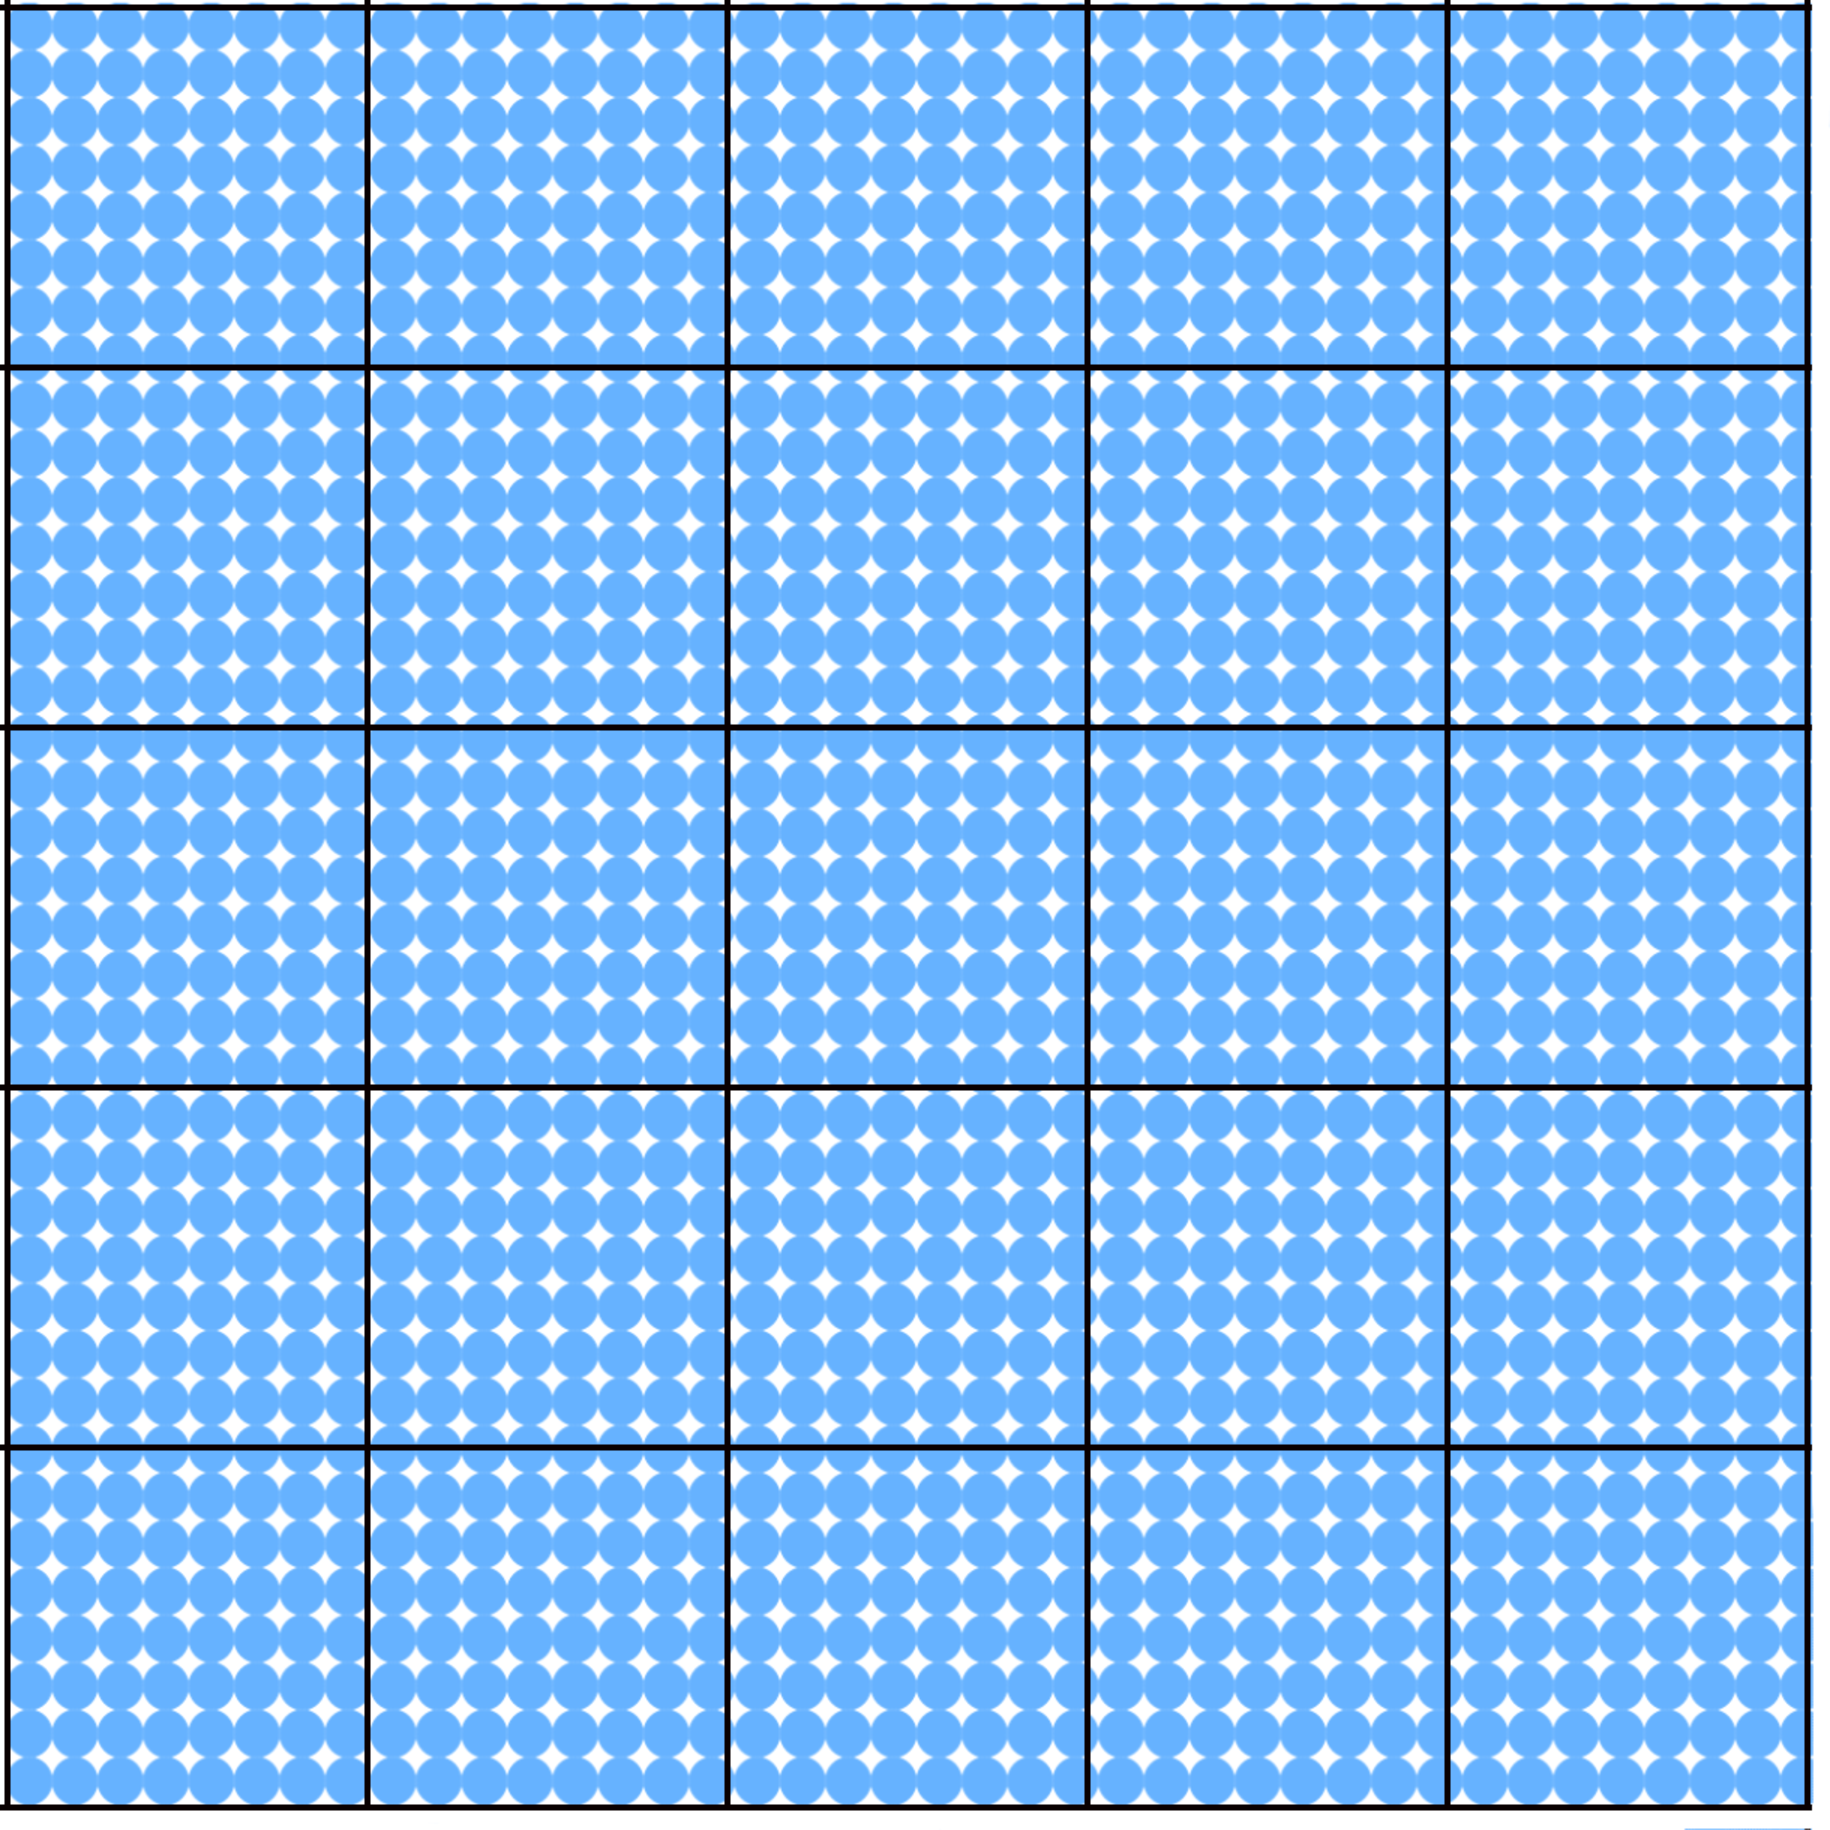
\includegraphics[width=3.5cm, height=3.5cm]{fig/SVD_1_grid}
    \caption{\label{fig:SVD_initial}Full $5\times 5$ tile matrix.}
  \end{subfigure}
  \hfill
  \begin{subfigure}[t]{0.3 \textwidth}
    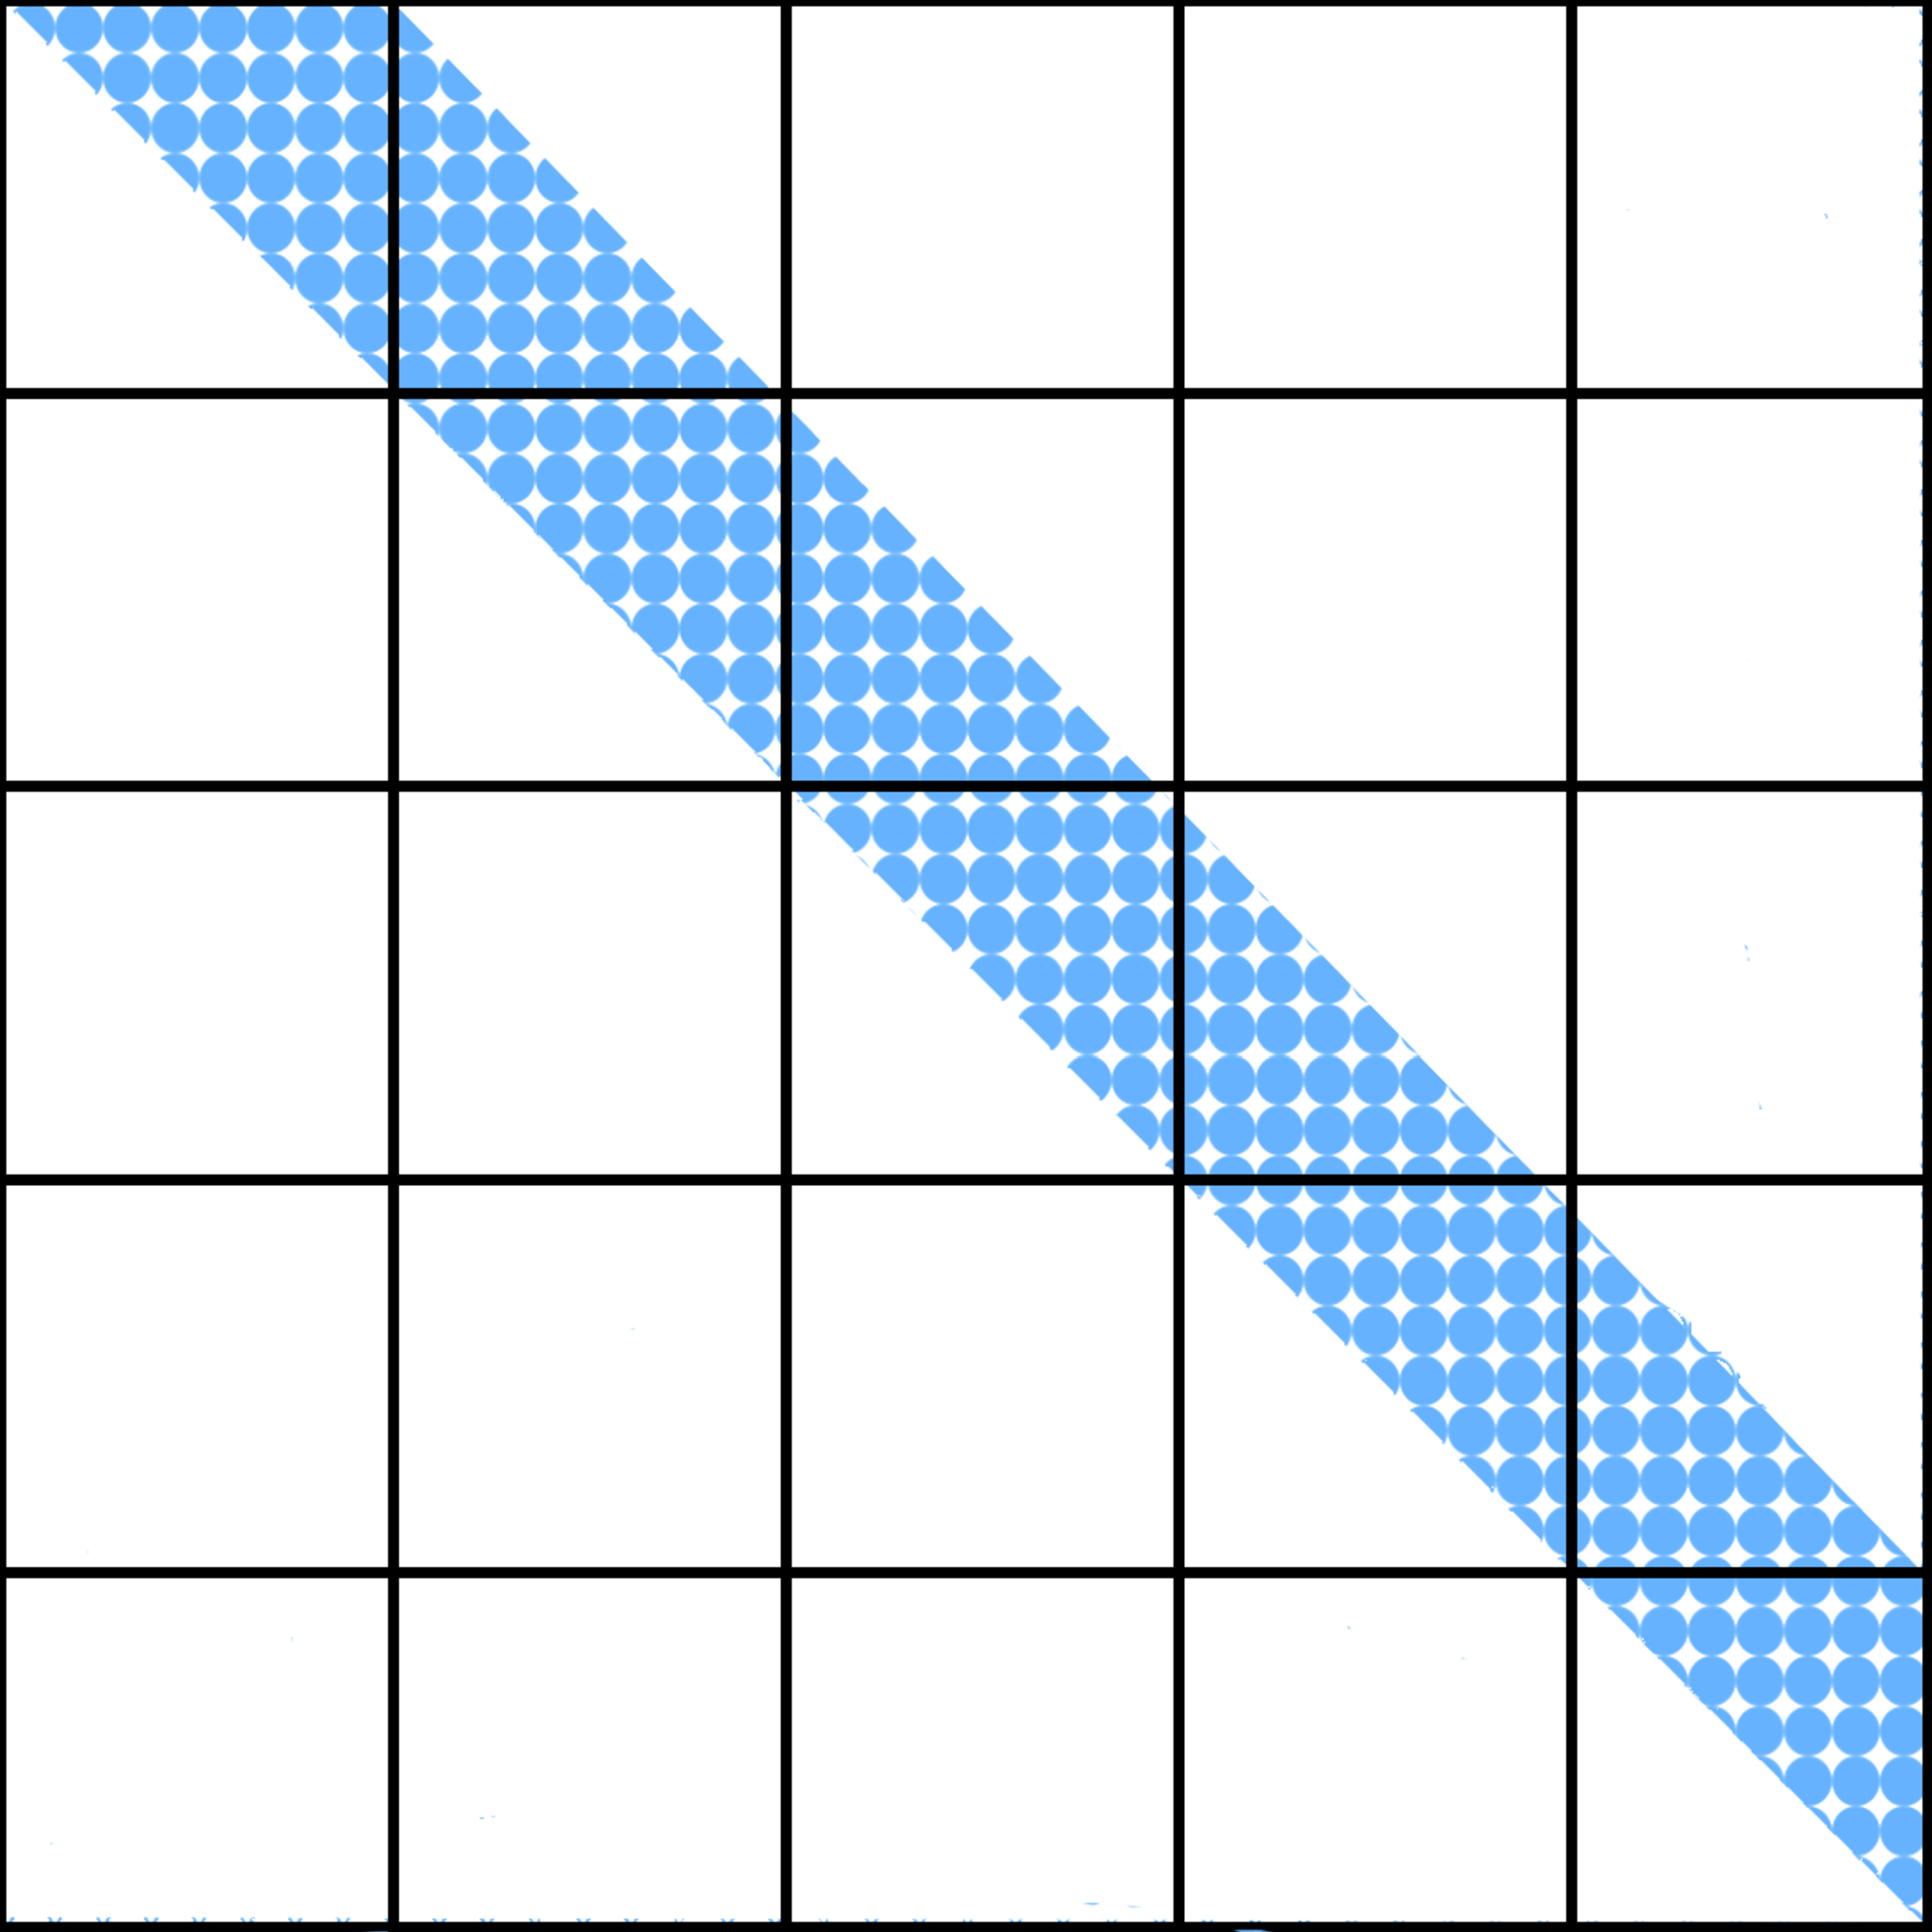
\includegraphics[width=3.5cm, height=3.5cm]{fig/SVD_band_bidiag}
    \caption{\label{fig:SVD_band_bidiag}
     Band bidiagonal form.}
  \end{subfigure}
  \hfill
    \begin{subfigure}[t]{0.3 \textwidth}
    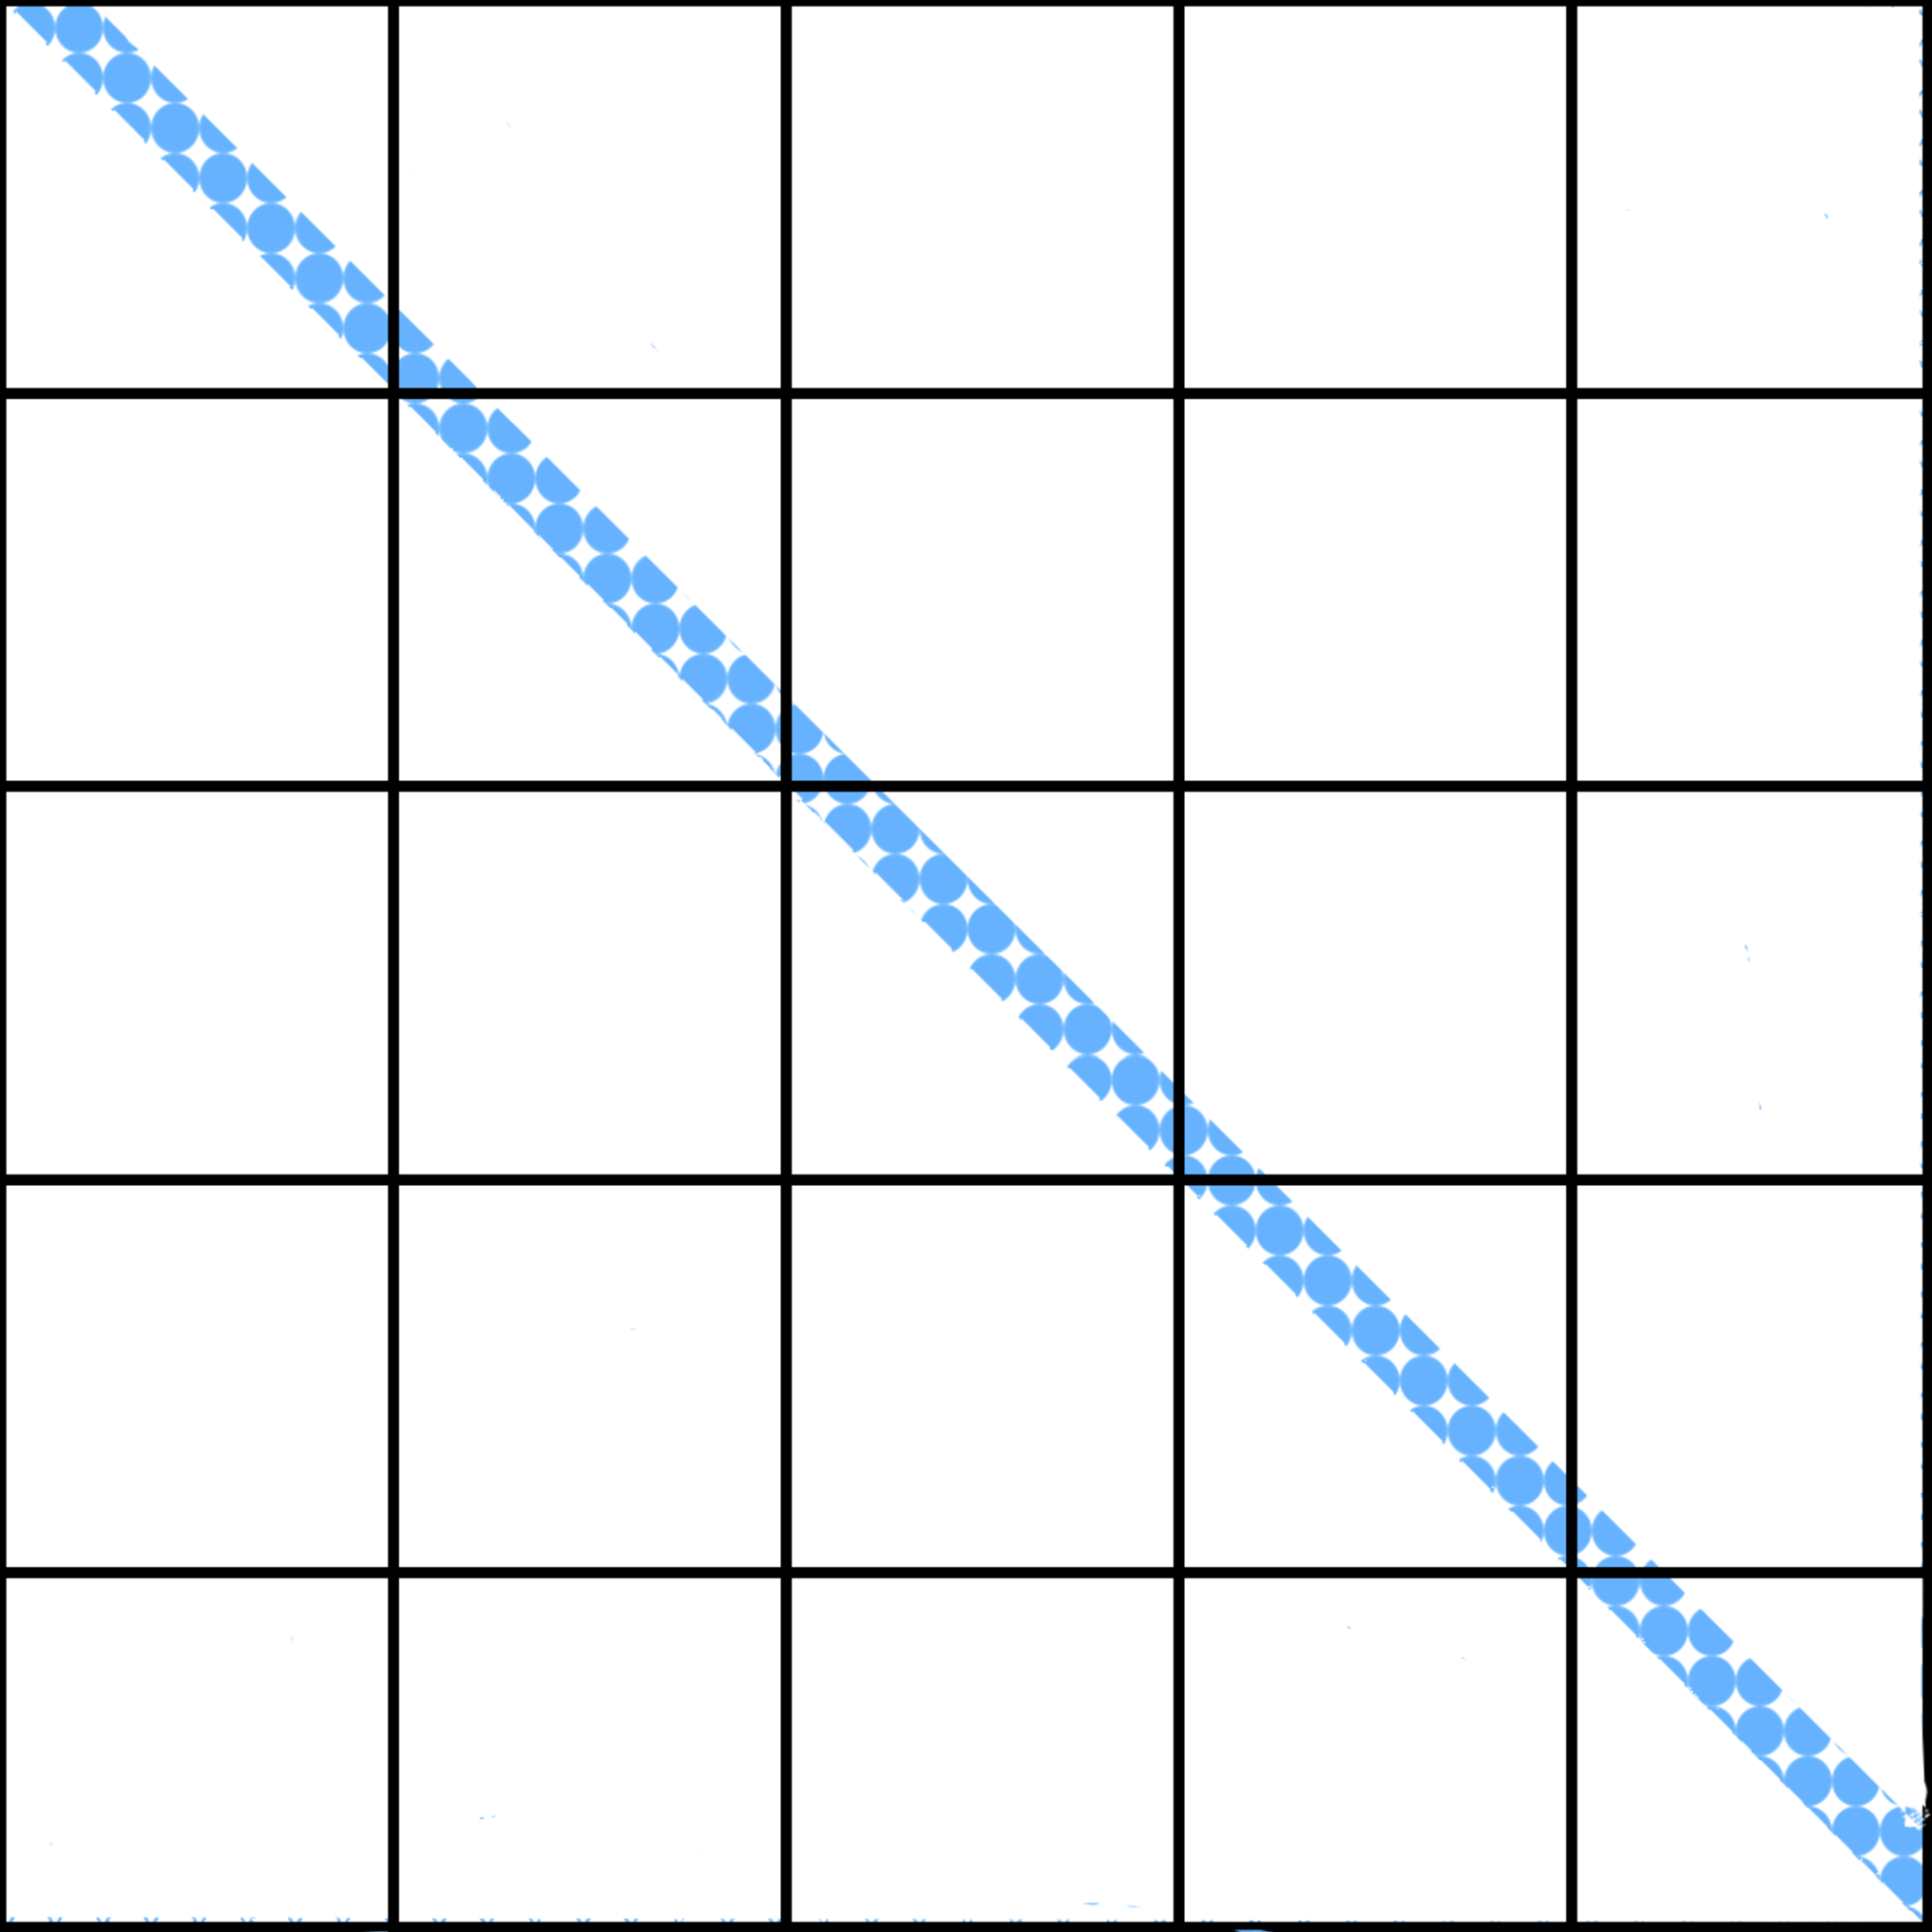
\includegraphics[width=3.5cm, height=3.5cm]{fig/SVD_bidiag}
    \caption{\label{fig:SVD_bidiag}
     Bidiagonal form.}
    \end{subfigure}
    \caption{Illustration of the two-stage bidiagonal reduction process.}
    \label{fig:two_stage}
\end{figure}

\section{Principles of tile algorithms}\label{sec:tile}
In order to use modern many/multi-core shared memory architectures at
full efficiency,
many LAPACK library algorithms initially powered by
block algorithms have been redesigned into tile algorithms.
This led to a new generation of linear algebra libraries such as
PLASMA~\cite{DBLP:journals/corr/abs-0709-1272} and FLAME~\cite{FLAWN3}.
The key idea is that,
instead of operating on block-columns as found in LAPACK,
tile algorithms operates at a finer granularity by dividing the whole
matrix into small square tiles which are more likely to fit into the
L2 cache of a CPU.
As illustrated in Figure~\ref{fig:SVD_initial}, the original
matrix has been converted into a 5-by-5 tile matrix.  One of the
advantages of working at tile granularity is that it provides more
room for parallelism with many tasks to keep all computational cores
busy.

Another advantage of tile algorithms is that they alleviate
the fork-join overhead inherent to parallelized LAPACK
block algorithms~\cite{haidar2012analysis}.
In fact,
the order of execution of the tasks in tile algorithms are commonly
represented in form of a Directed Acyclic Graph (DAG) where each node
represents a task, while the edges represent the
data dependencies between the tasks.
These tasks are then scheduled
thanks to a runtime system which checks the dependencies and
takes care of launching tasks on appropriate cores.

  \begin{figure}[h!]
    %%%% 1
    \captionsetup[subfigure]{justification=justified,singlelinecheck=false}
  \begin{subfigure}[t]{0.160 \textwidth}
    
\includegraphics[width=0.7cm, height=3.5cm]{fig/SVD_rect_panel_1}
    \caption{\label{fig:geqrt_1}QR}
  \end{subfigure}
  \hfill
  %%%% 2
  \begin{subfigure}[t]{0.160 \textwidth}
    
\includegraphics[width=0.7cm, height=3.5cm]{fig/SVD_rect_panel_3}
    \caption{\label{fig:tsqrt_2}TSQRT}
  \end{subfigure}
  \hfill
  %%%% 3
    \begin{subfigure}[t]{0.160 \textwidth}
    
\includegraphics[width=0.7cm, height=3.5cm]{fig/SVD_rect_panel_5}
    \caption{\label{fig:tsqrt_3} TSQRT}
    \end{subfigure}
    \hfill
    %%%% 4
    \begin{subfigure}[t]{0.160 \textwidth}
      
\includegraphics[width=0.7cm, height=3.5cm]{fig/SVD_rect_panel_6}
      \caption{\label{fig:tsqrt_4}TSQRT}
    \end{subfigure}
    \hfill
    %%%% 5
    \begin{subfigure}[t]{0.160 \textwidth}
      
\includegraphics[width=0.7cm, height=3.5cm]{fig/SVD_rect_panel_7}
      \caption{\label{fig:tsqrt_5}TSQRT}
    \end{subfigure}
    \hfill
    %%%% 6
    \begin{subfigure}[t]{0.160 \textwidth}
      
\includegraphics[width=0.7cm, height=3.5cm]{fig/SVD_rect_panel_8}
      \caption{\label{fig:tsqrt_output}End}
    \end{subfigure}
    \caption{Panel factorization using the triangle on top of square QR factorization kernel (TSQRT).
    \label{fig:rect_panel}}
\end{figure}

For the sake of illustration, Figure~\ref{fig:rect_panel}
shows the tile algorithm variant of QR factorization for a panel
(block-column).
Following the example shown in
Figure~\ref{fig:two_stage}, the panel has been divided into 5 tiles.
This algorithm involves two tile kernels:
a standard QR factorization kernel to
factorize the top-most tile (Figure~\ref{fig:geqrt_1}),
and a specialized kernel to use the top triangular matrix
from the first QR factorization
to eliminate the square tiles below (Figures~\ref{fig:tsqrt_2}-\ref{fig:tsqrt_5}).
This kernel is denoted TSQRT and stands
for ``triangle on top of square tile QR factorization''.
In the next few sections we will introduce other specialized kernels,
designed to operate on tiles.

\section{Reduction  to band bidiagonal form}
\label{sec:band}
The idea of using a tile algorithm to factorize a full matrix into
band bidiagonal is not new.
The approach was first introduced in 2010 by
Dongarra~et~al\@.~\cite{ltaief2010parallel},
and improved in 2013~\cite{haidar2013improved}
by the same authors.
This section aims at evaluating different options for
designing such an algorithm
before moving to the second stage of the factorization.

We identified two main design options:
(1) a ``late update'' strategy, and
(2) an ``early update'' strategy.
Each of these strategies are introduced
and assessed in the subsections below.

\subsection{Late update strategy}
To reduce a full $mt \times nt$ tile matrix $A$ to a band bidiagonal
form, the late update strategy begins by applying a QR
factorization to the first panel $A(1:mt,1)$ (using MATLAB indexing)
(see Figure~\ref{fig:qr_1}), then updating the trailing
submatrix $A(1:mt,2:nt)$ (Figure~\ref{fig:qr_update_1}), followed
by an LQ factorization of the first tile-row,
ignoring the first column (Figure~\ref{fig:lq_1}),
and the update of the corresponding trailing matrix
(Figure~\ref{fig:lq_update_1}).
This procedure is repeated until the whole matrix is reduced to
band bidiagonal form, as illustrated in Figure~\ref{fig:panel}.
It is important to notice that we describe this strategy
at tile-column (panel) and tile-row granularity but
tile algorithms are used underneath to process each panel
and the update of the trailing matrix.
We can think of this as a direct translation of the LAPACK
column-oriented procedure into a
more modern tile-based algorithm.

\begin{figure}[h!]
  %%%% 1
  \captionsetup[subfigure]{justification=justified,singlelinecheck=false}

  \begin{subfigure}[t]{0.2 \textwidth}
    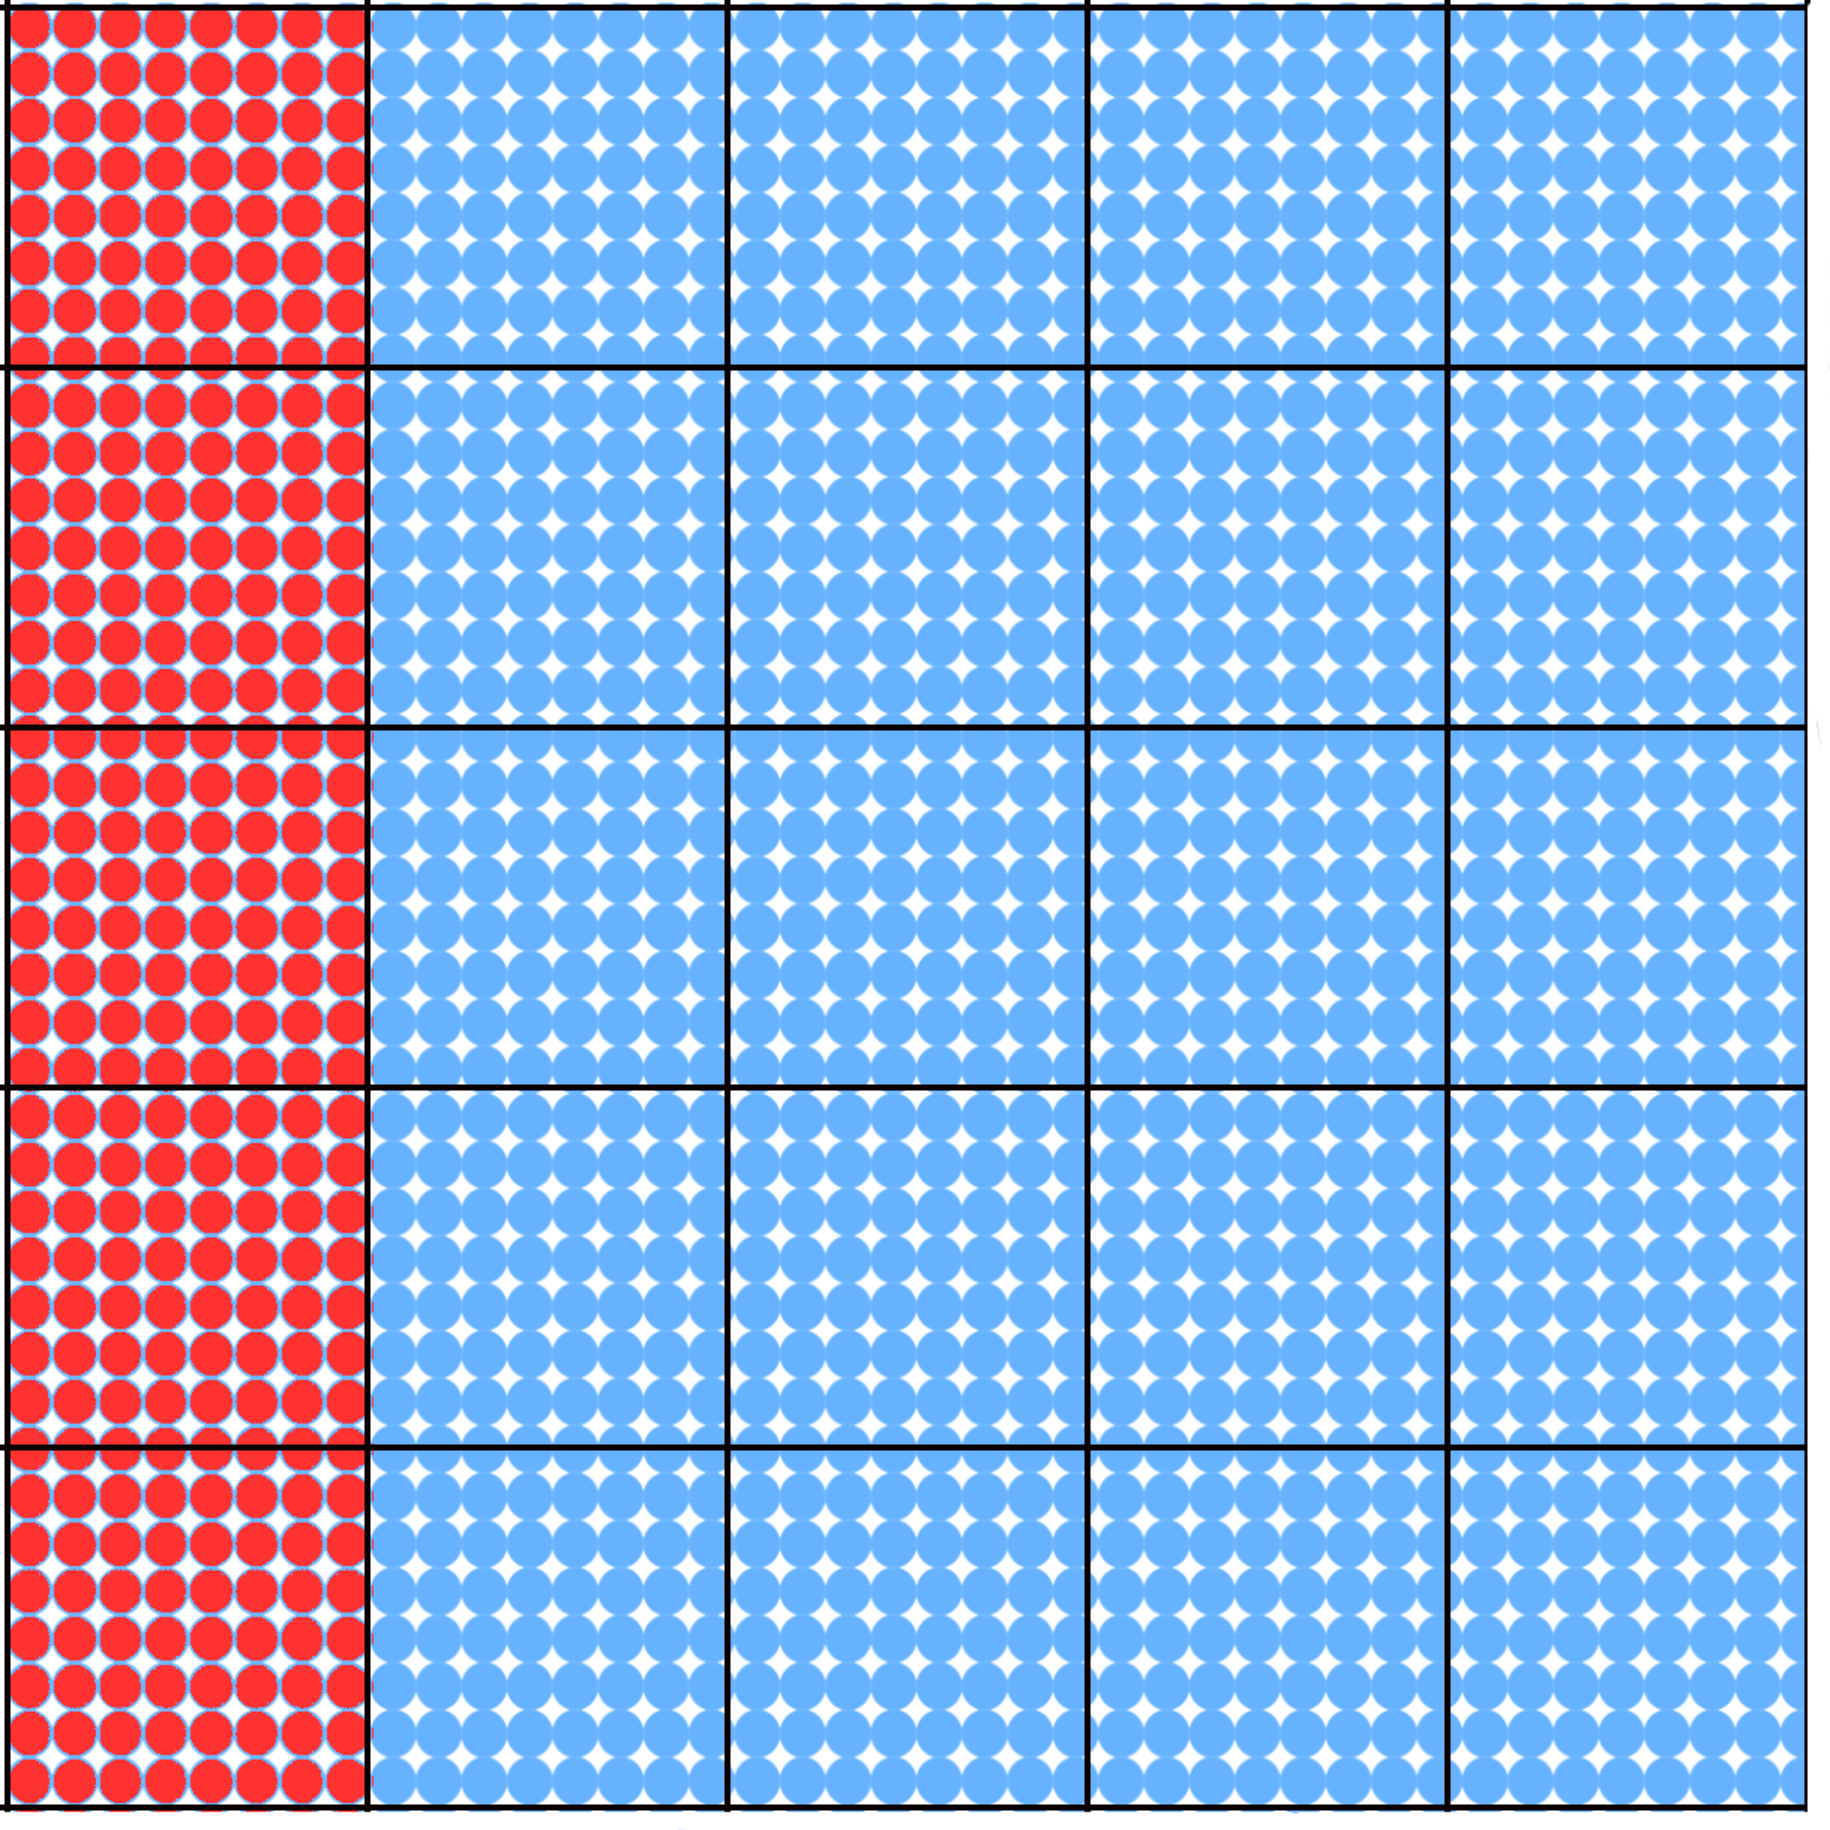
\includegraphics[width=\textwidth]{fig/SVD_panel_1_grid}
    \caption{\label{fig:qr_1}\small{Panel QR}}
  \end{subfigure}
  \hfill
  %%%% 2
  \begin{subfigure}[t]{0.2 \textwidth}
    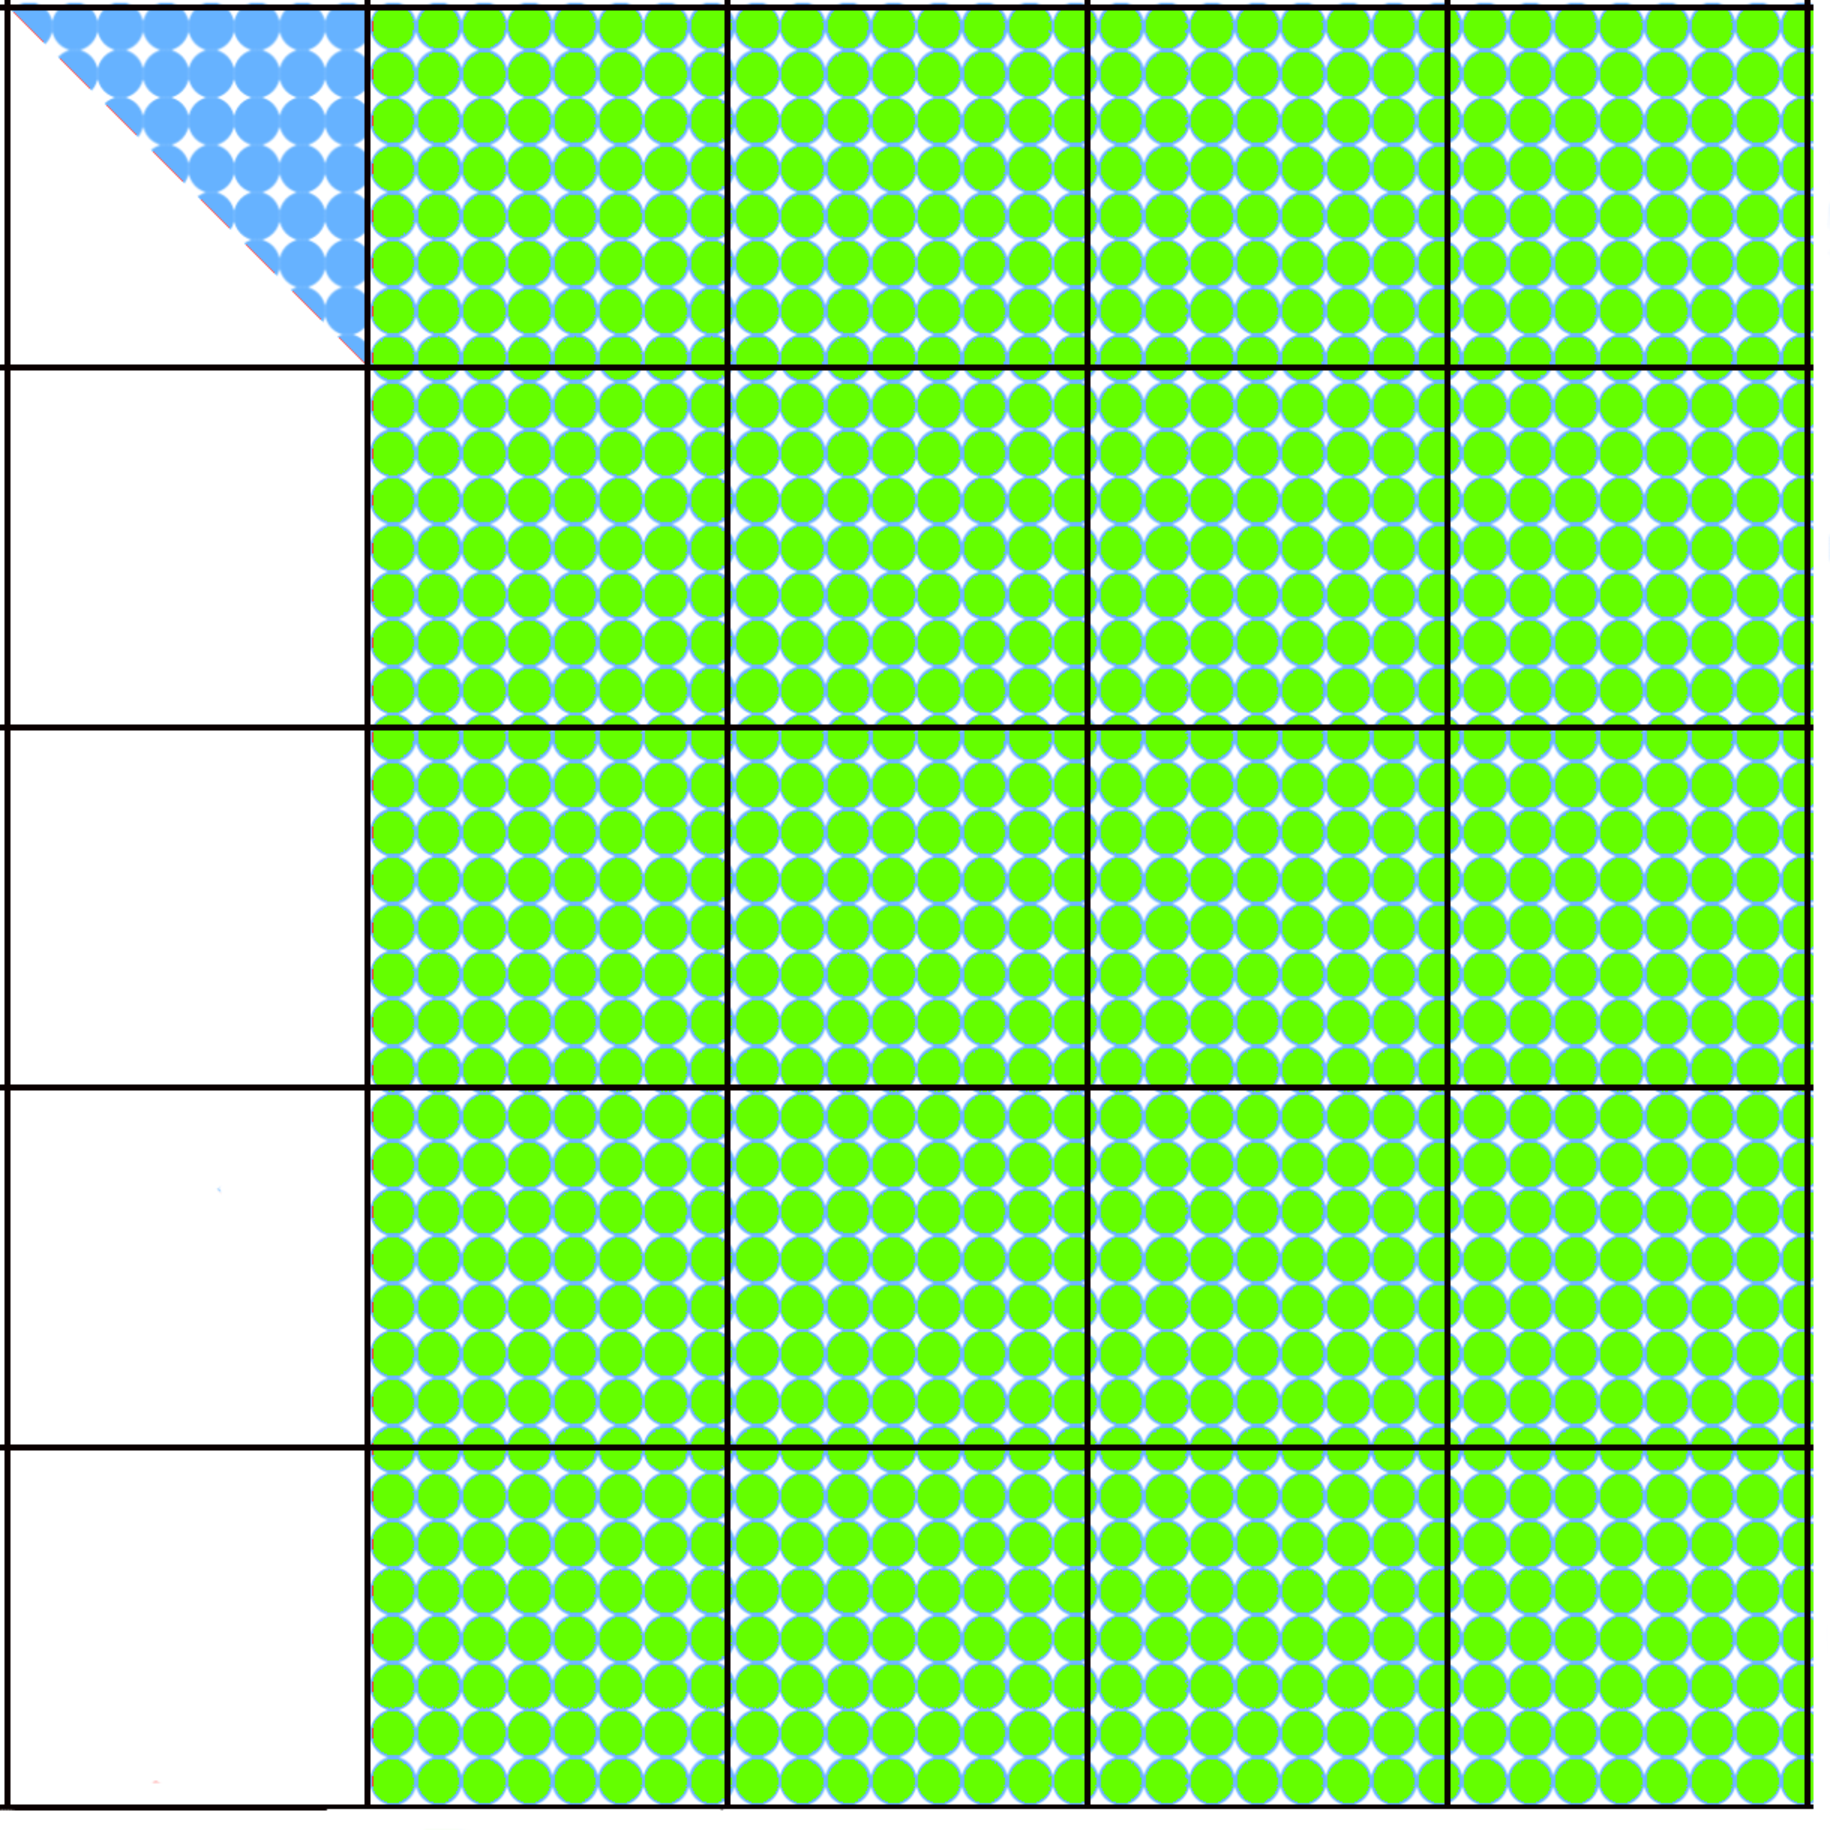
\includegraphics[width=\textwidth]{fig/SVD_panel_2_grid}
    \caption{\label{fig:qr_update_1}Update}
  \end{subfigure}
  \hfill
  %%%% 3
    \begin{subfigure}[t]{0.2 \textwidth}
    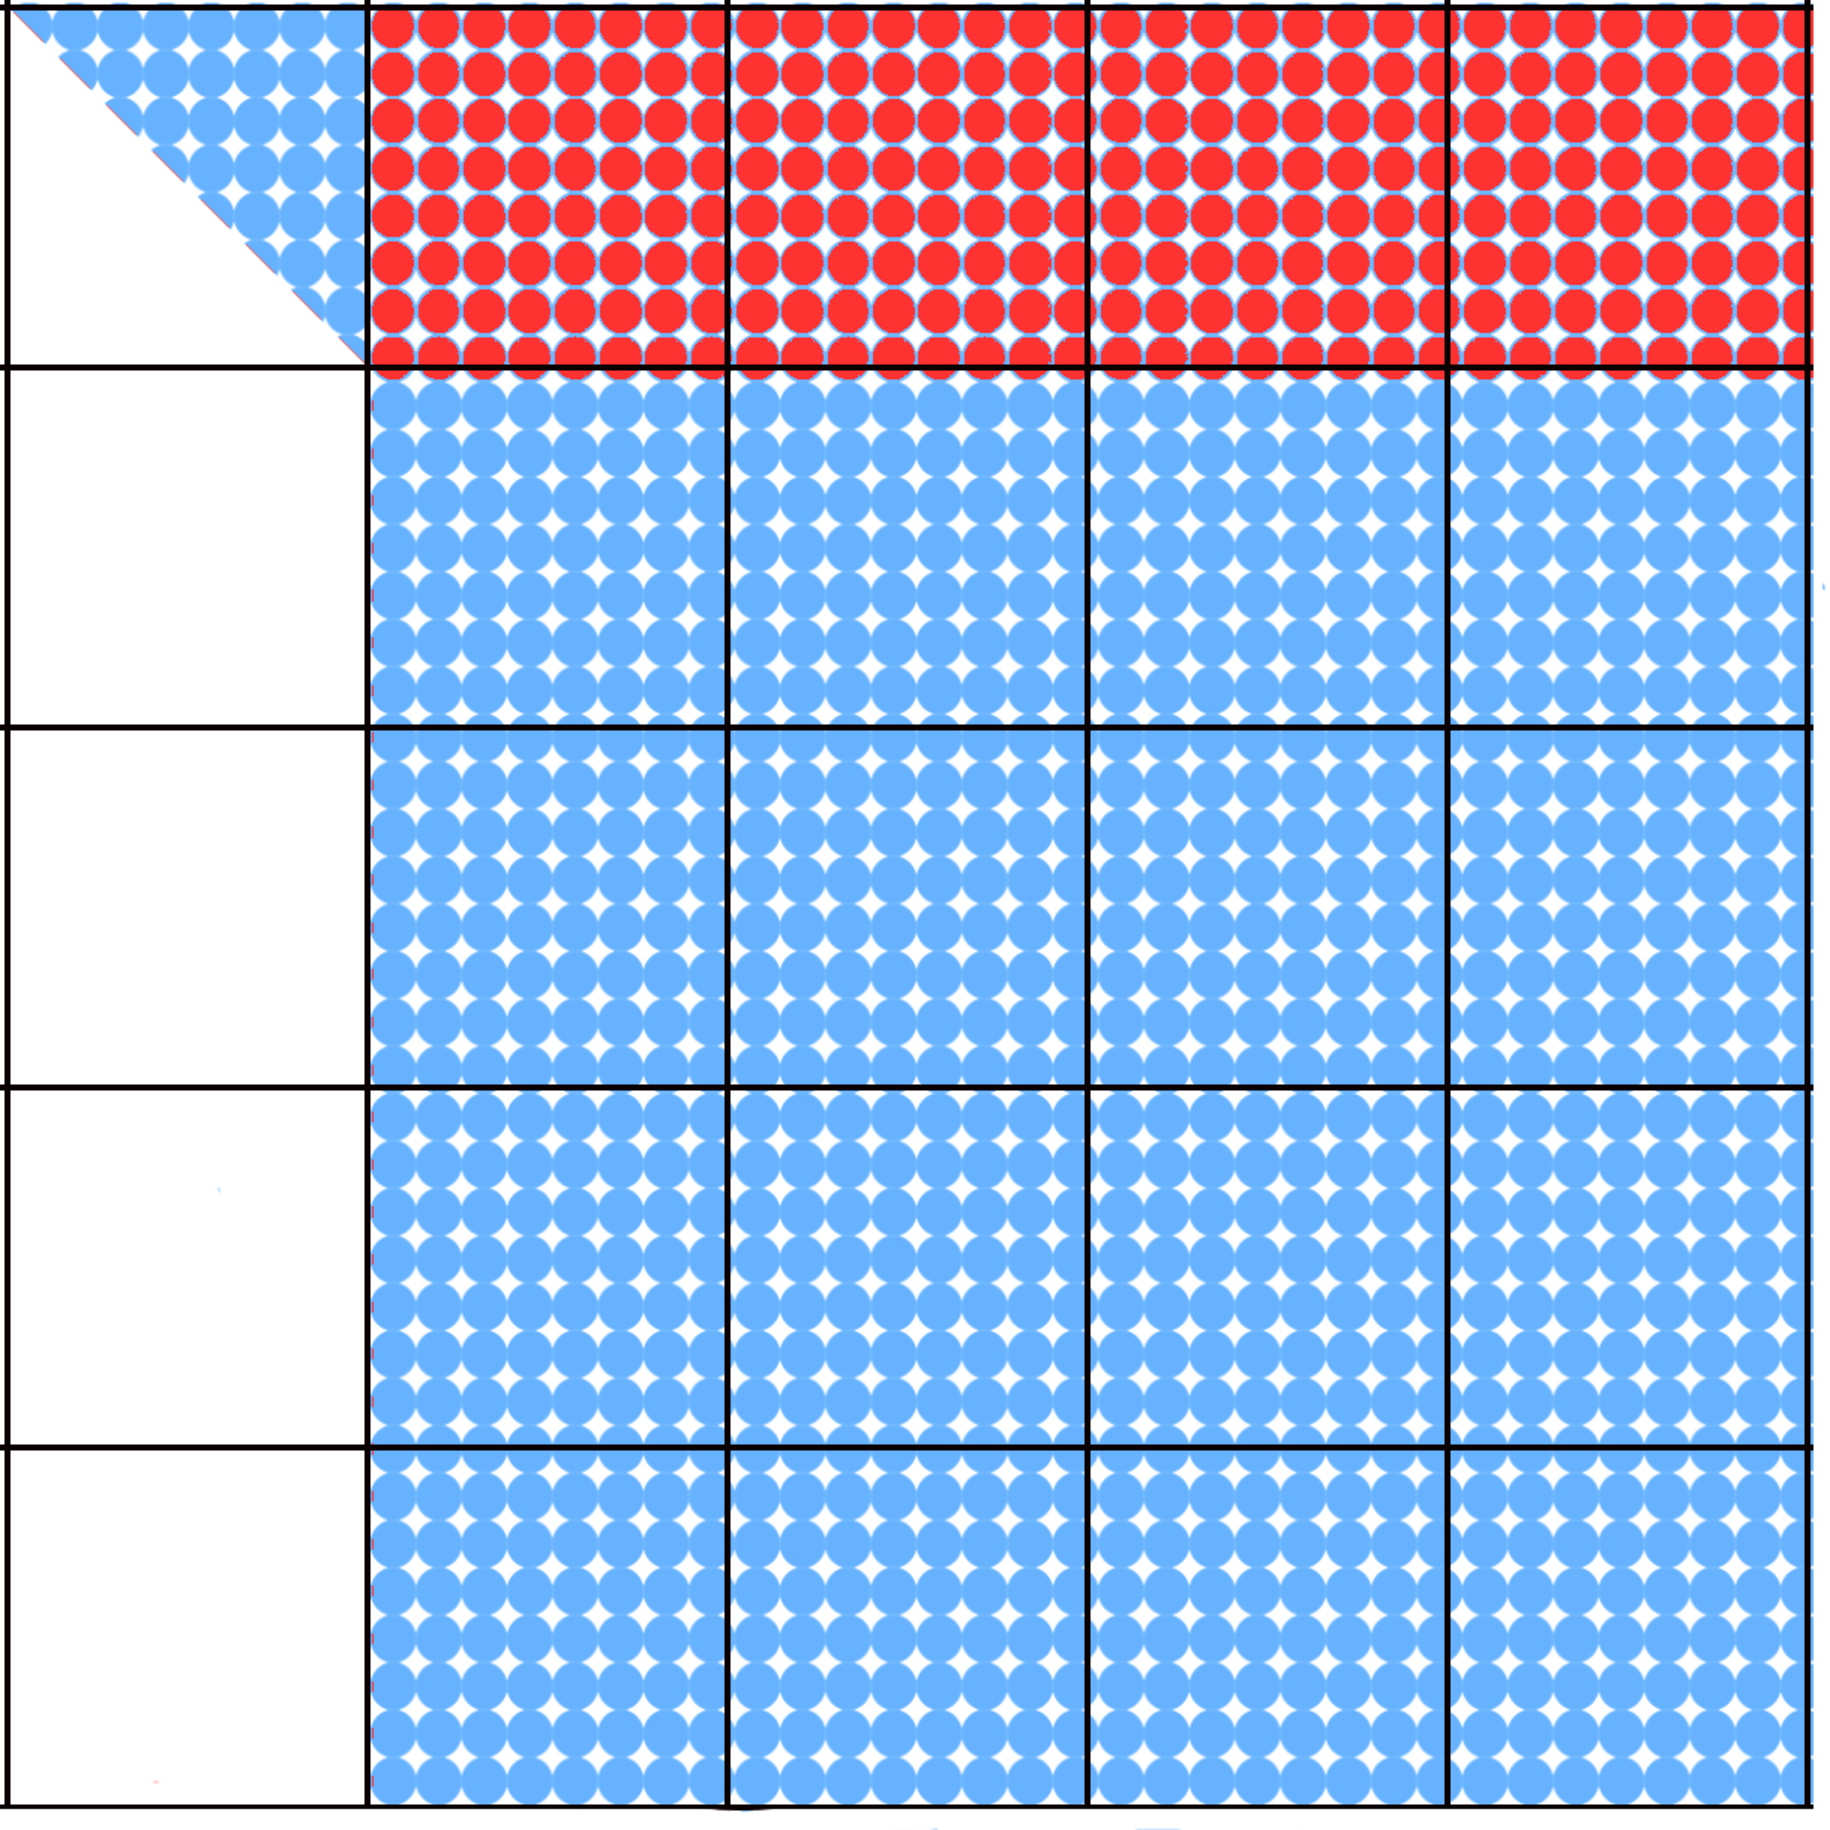
\includegraphics[width=\textwidth]{fig/SVD_panel_3_grid}
    \caption{\label{fig:lq_1}\small{Tile-row LQ}}
    \end{subfigure}
    \hfill
    %%%% 4
    \begin{subfigure}[t]{0.2 \textwidth}
      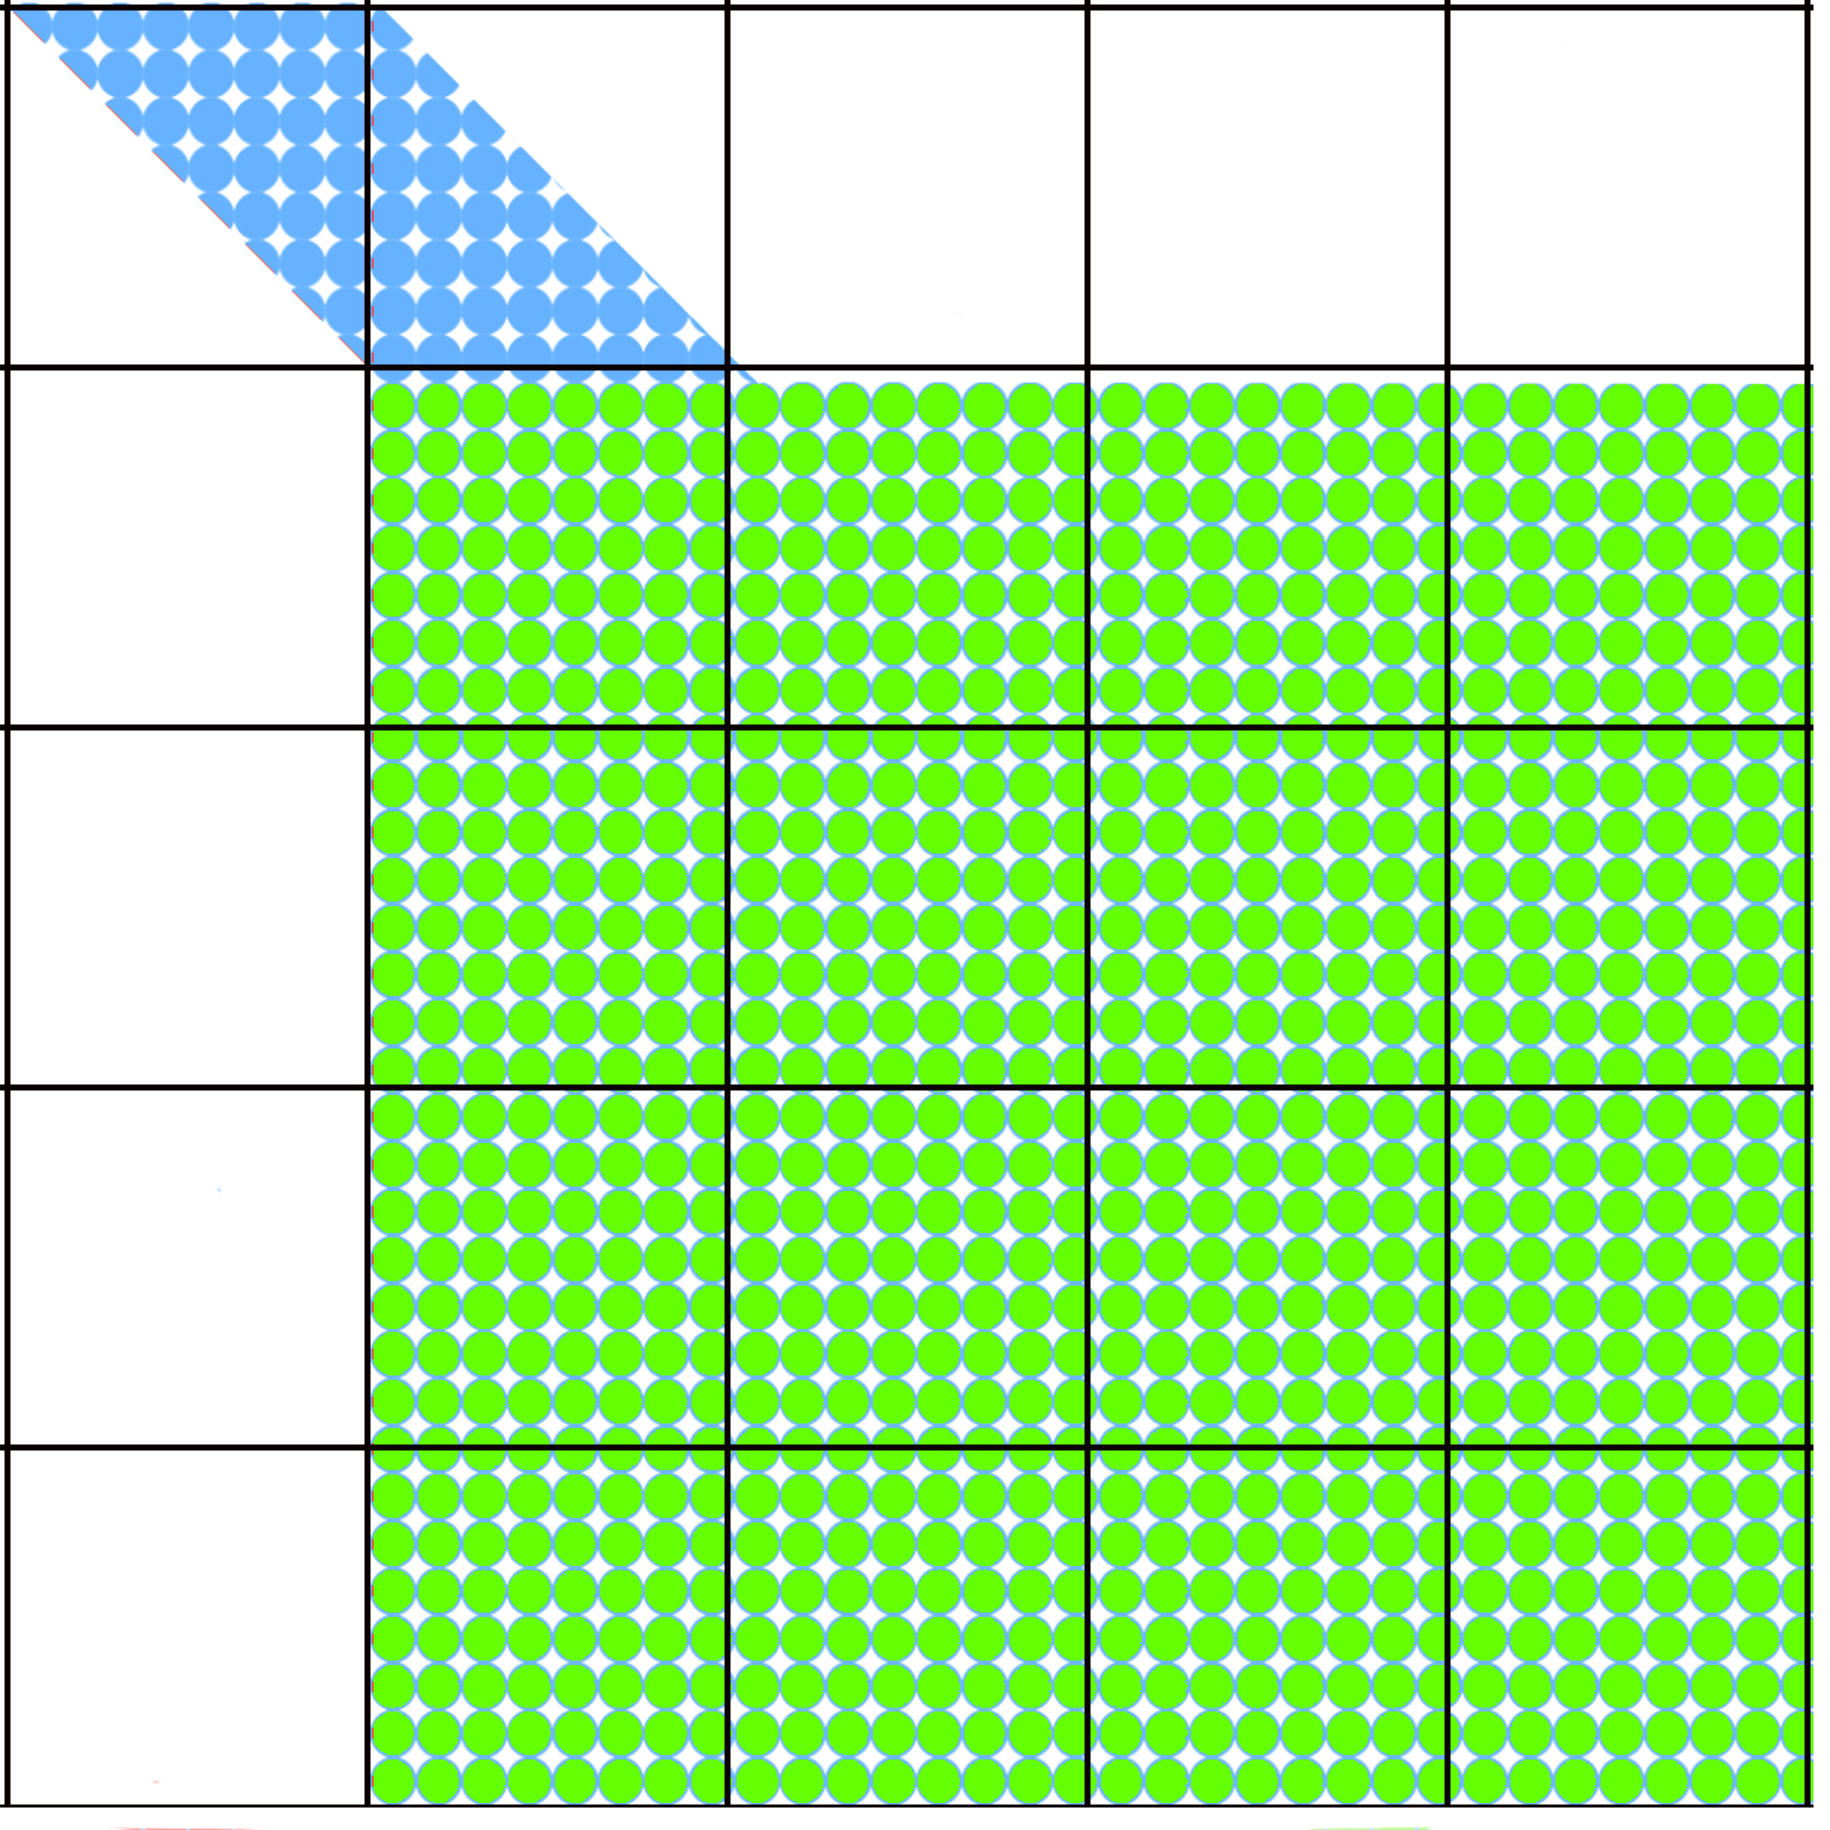
\includegraphics[width=\textwidth]{fig/SVD_panel_4_grid}
      \caption{\label{fig:lq_update_1}Update}
    \end{subfigure}
    \hfill
    %%%% 5
    \begin{subfigure}[t]{0.2 \textwidth}
      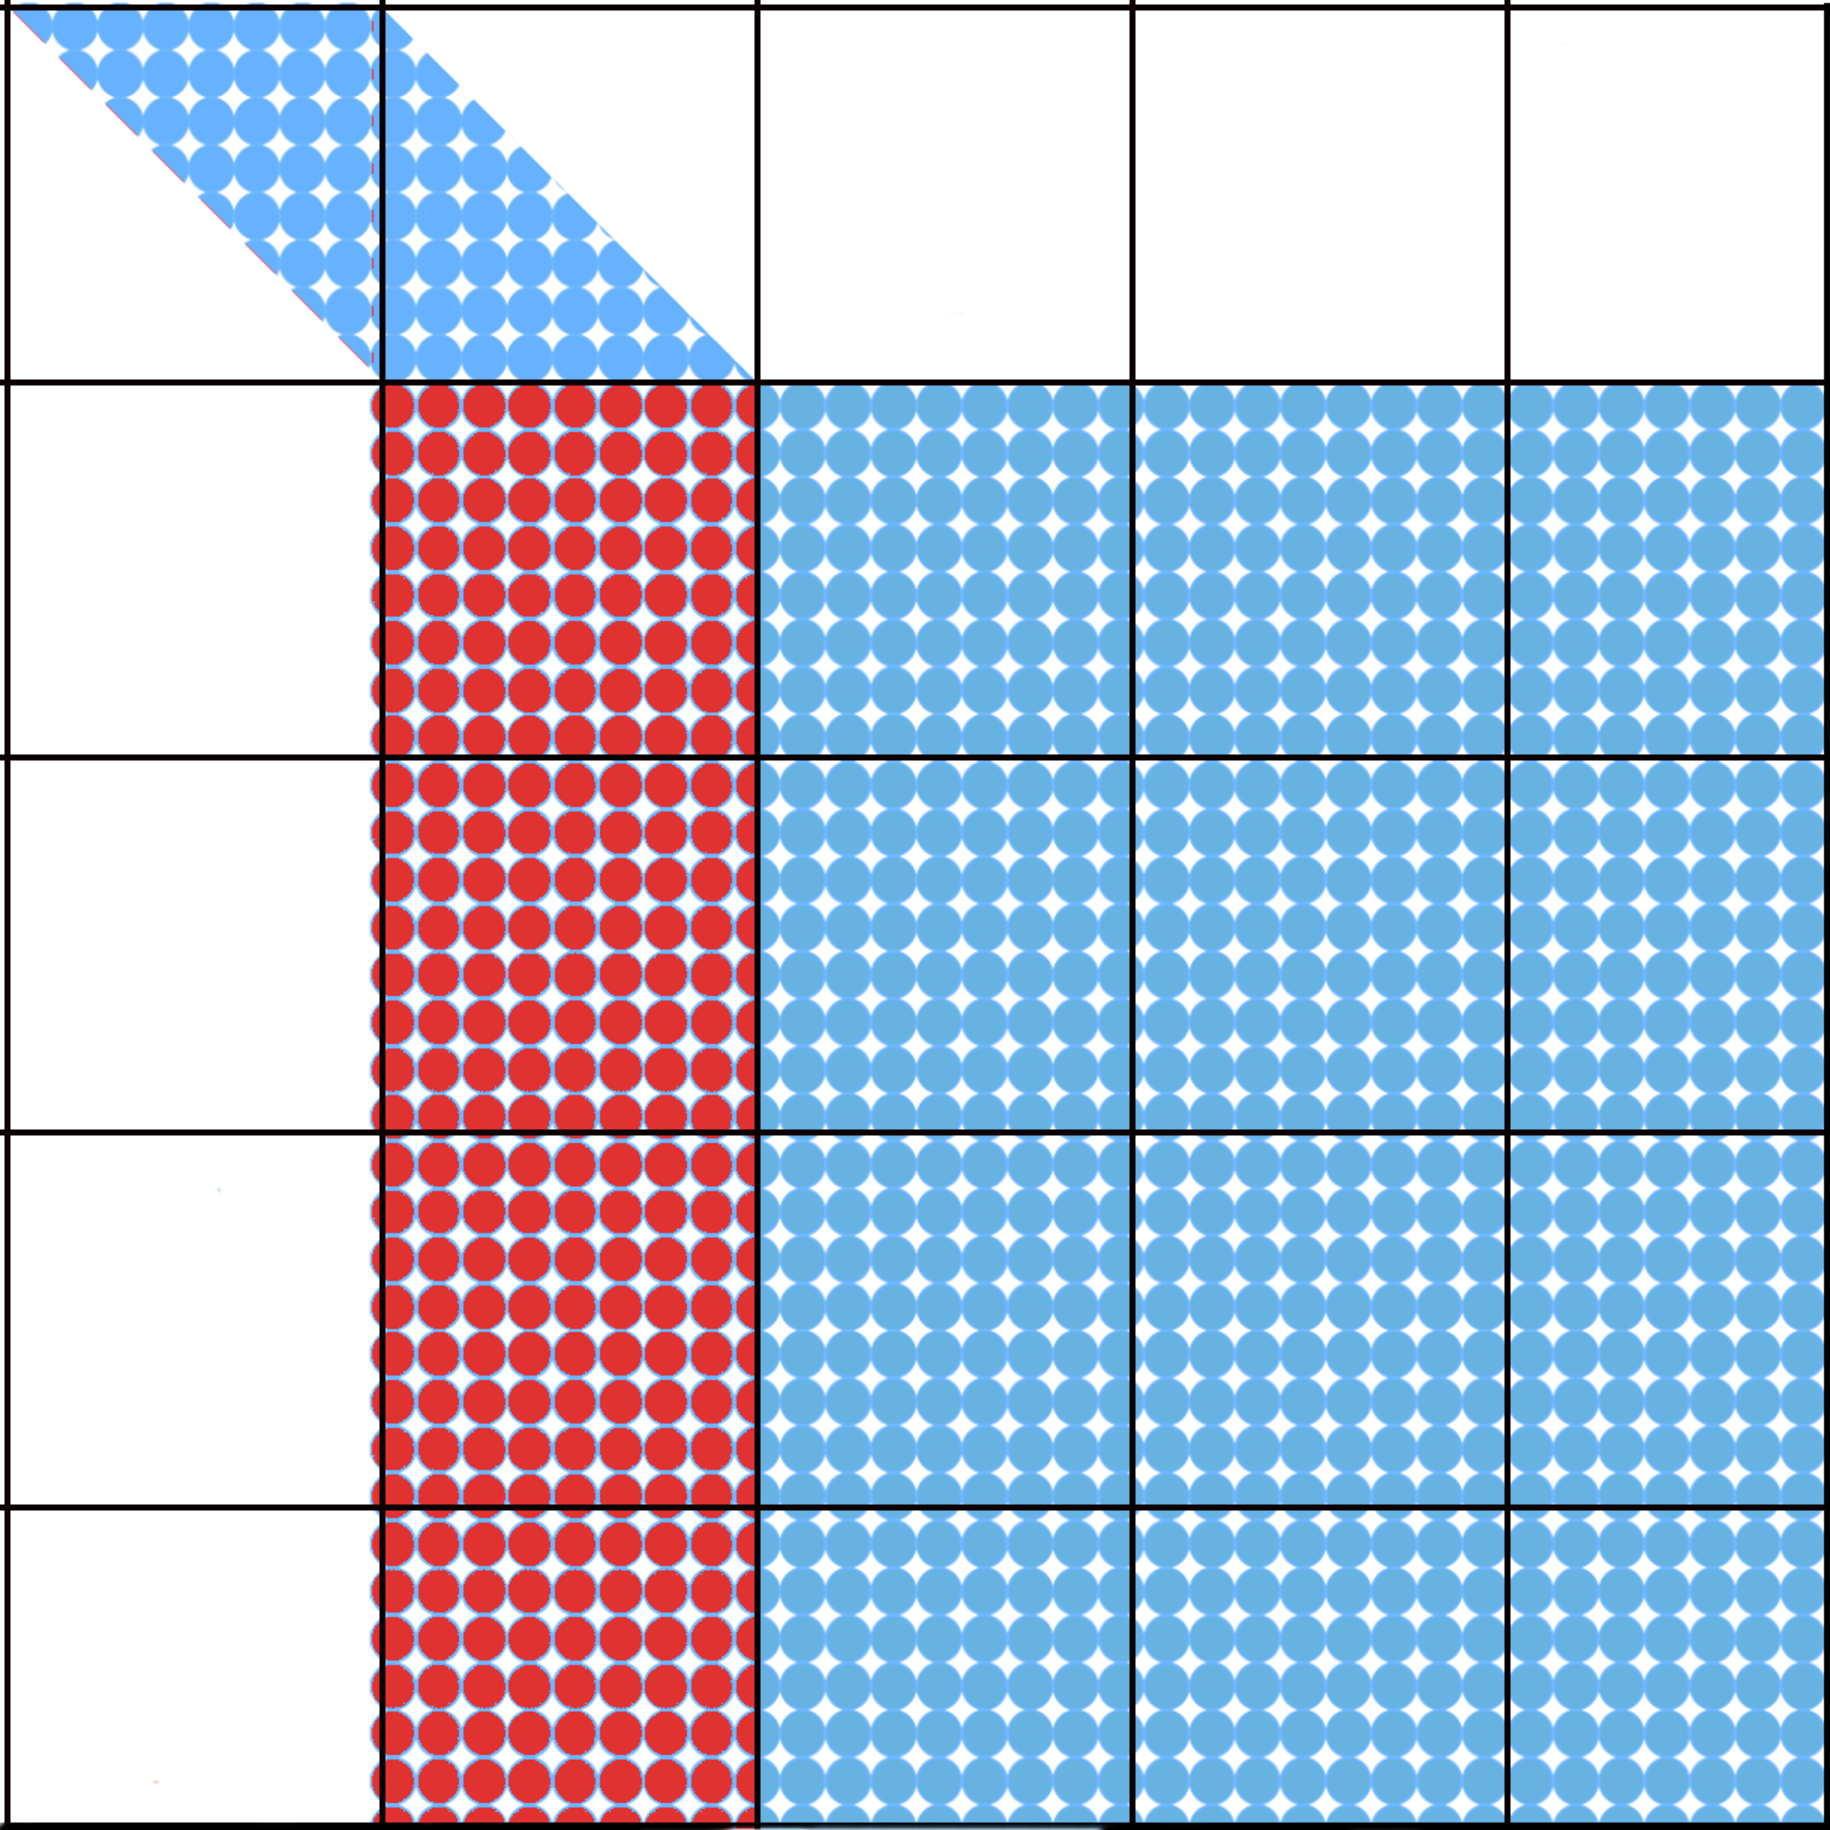
\includegraphics[width=\textwidth]{fig/SVD_panel_5_grid}
      \caption{\label{fig:qr_2}Panel QR}
    \end{subfigure}
    \hfill
    %%%% 6
    \begin{subfigure}[t]{0.2 \textwidth}
      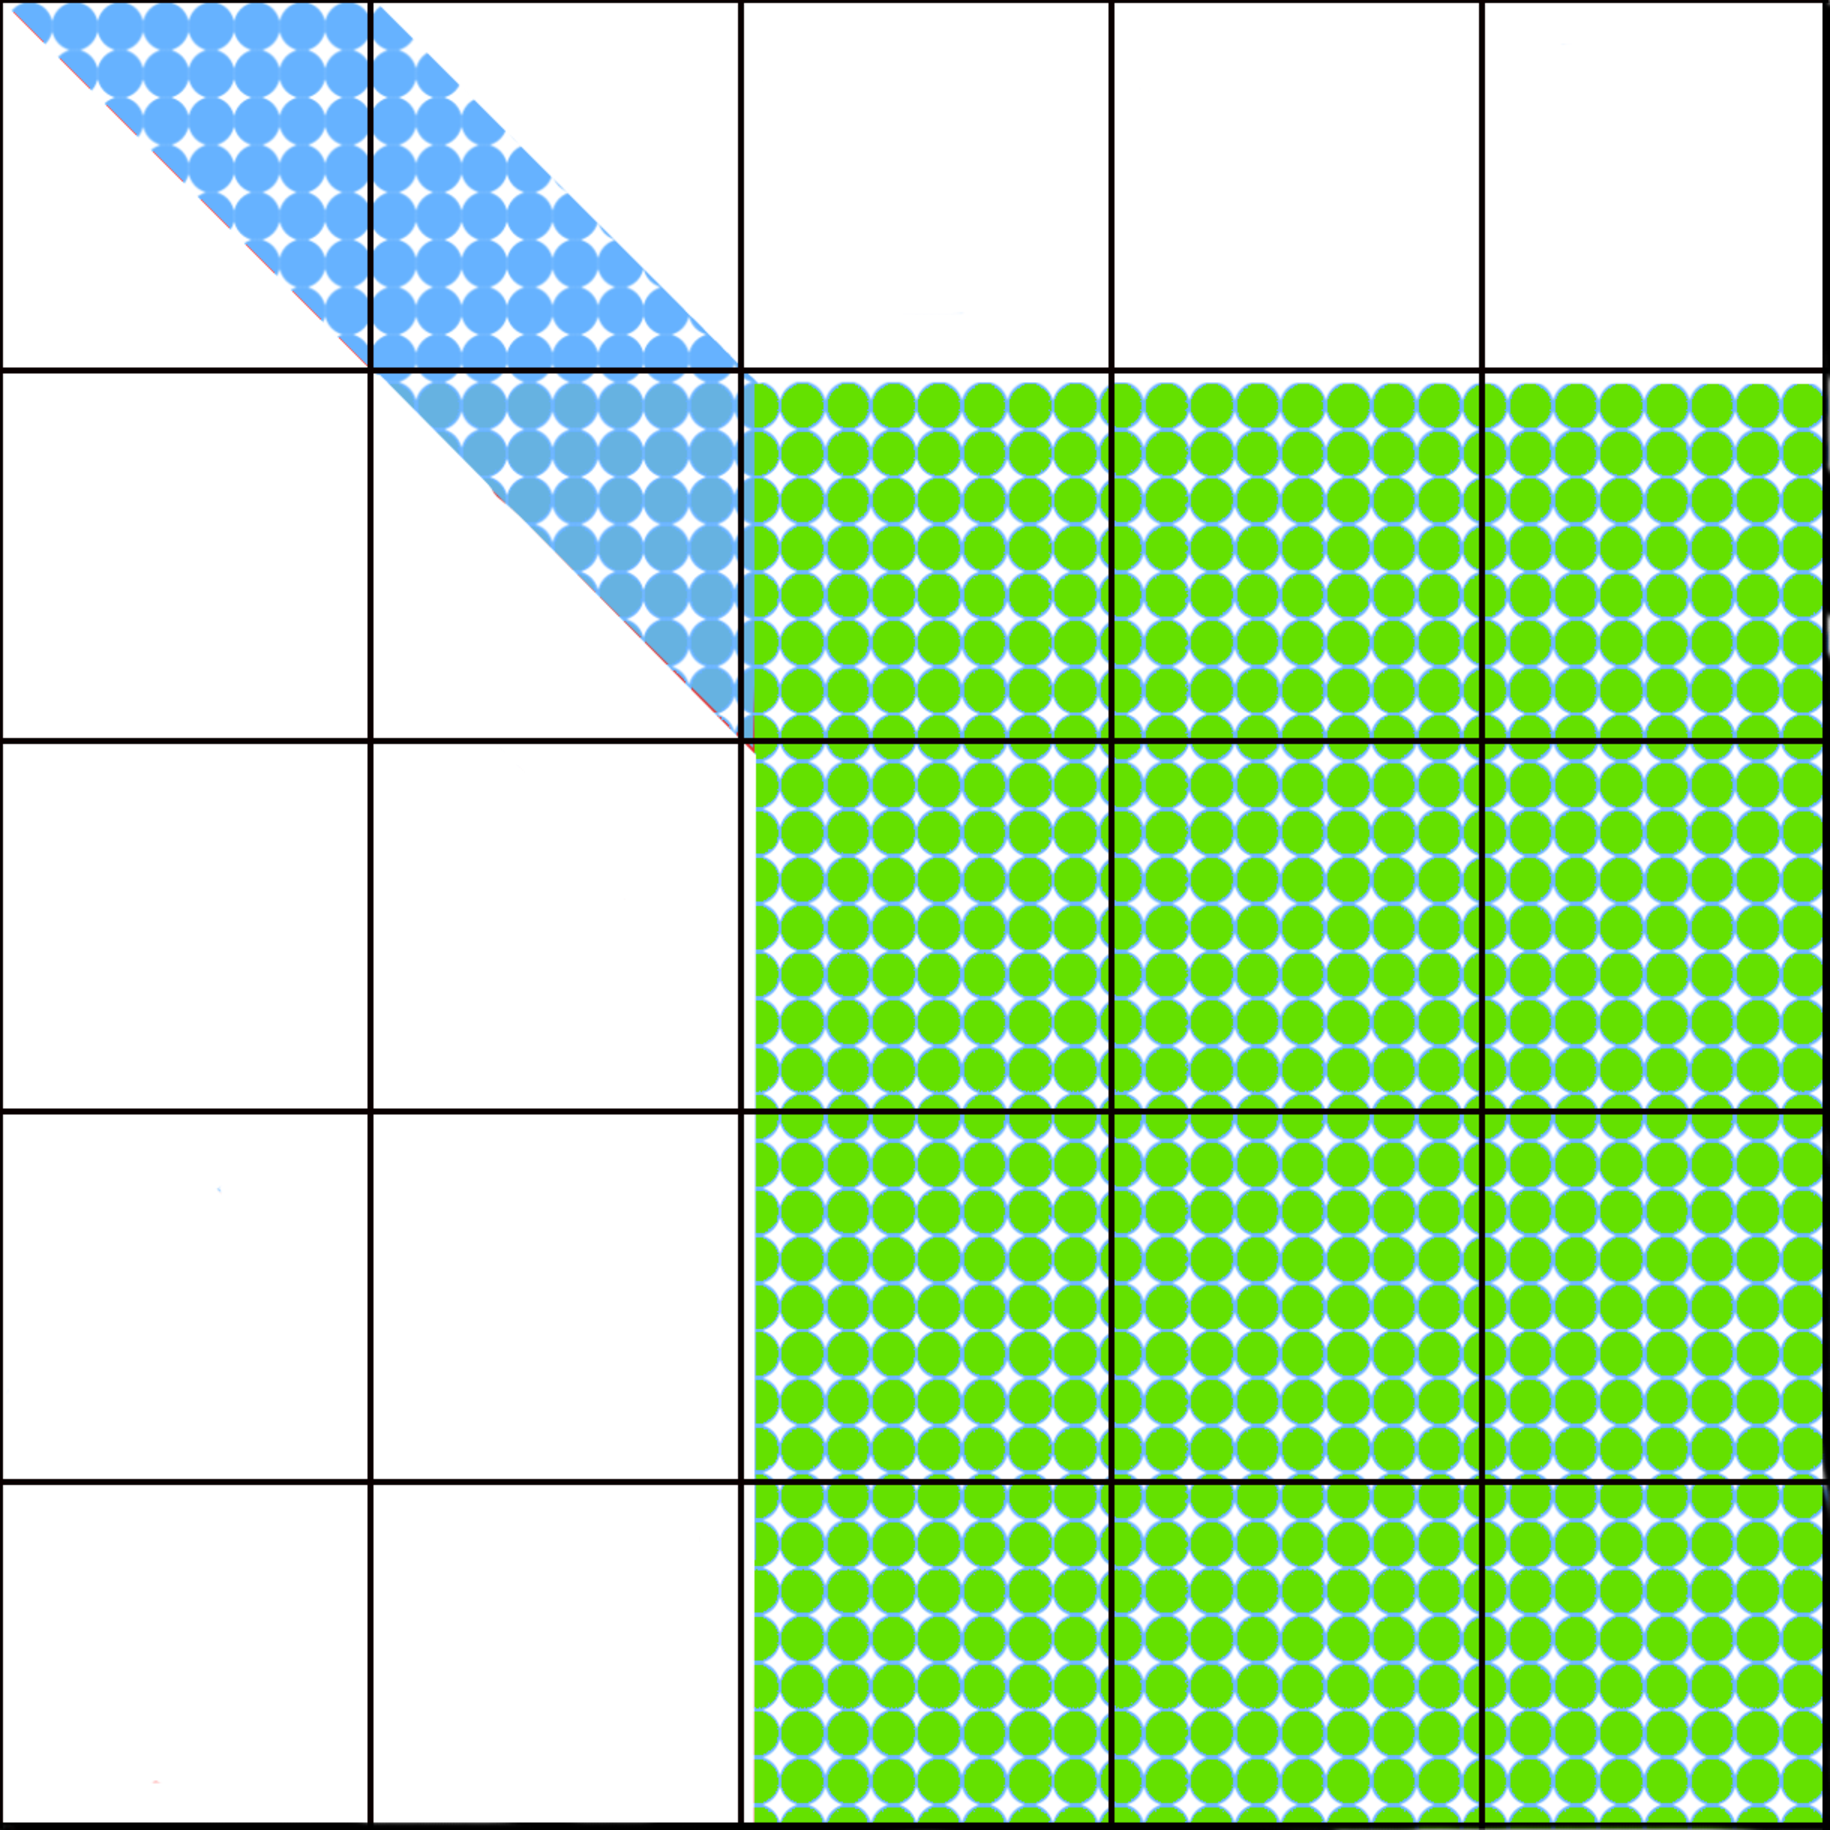
\includegraphics[width=\textwidth]{fig/SVD_panel_6_grid}
      \caption{\label{fig:qr_update_2}Update}
    \end{subfigure}
    \hfill
    %%%% 7
    \begin{subfigure}[t]{0.2 \textwidth}
      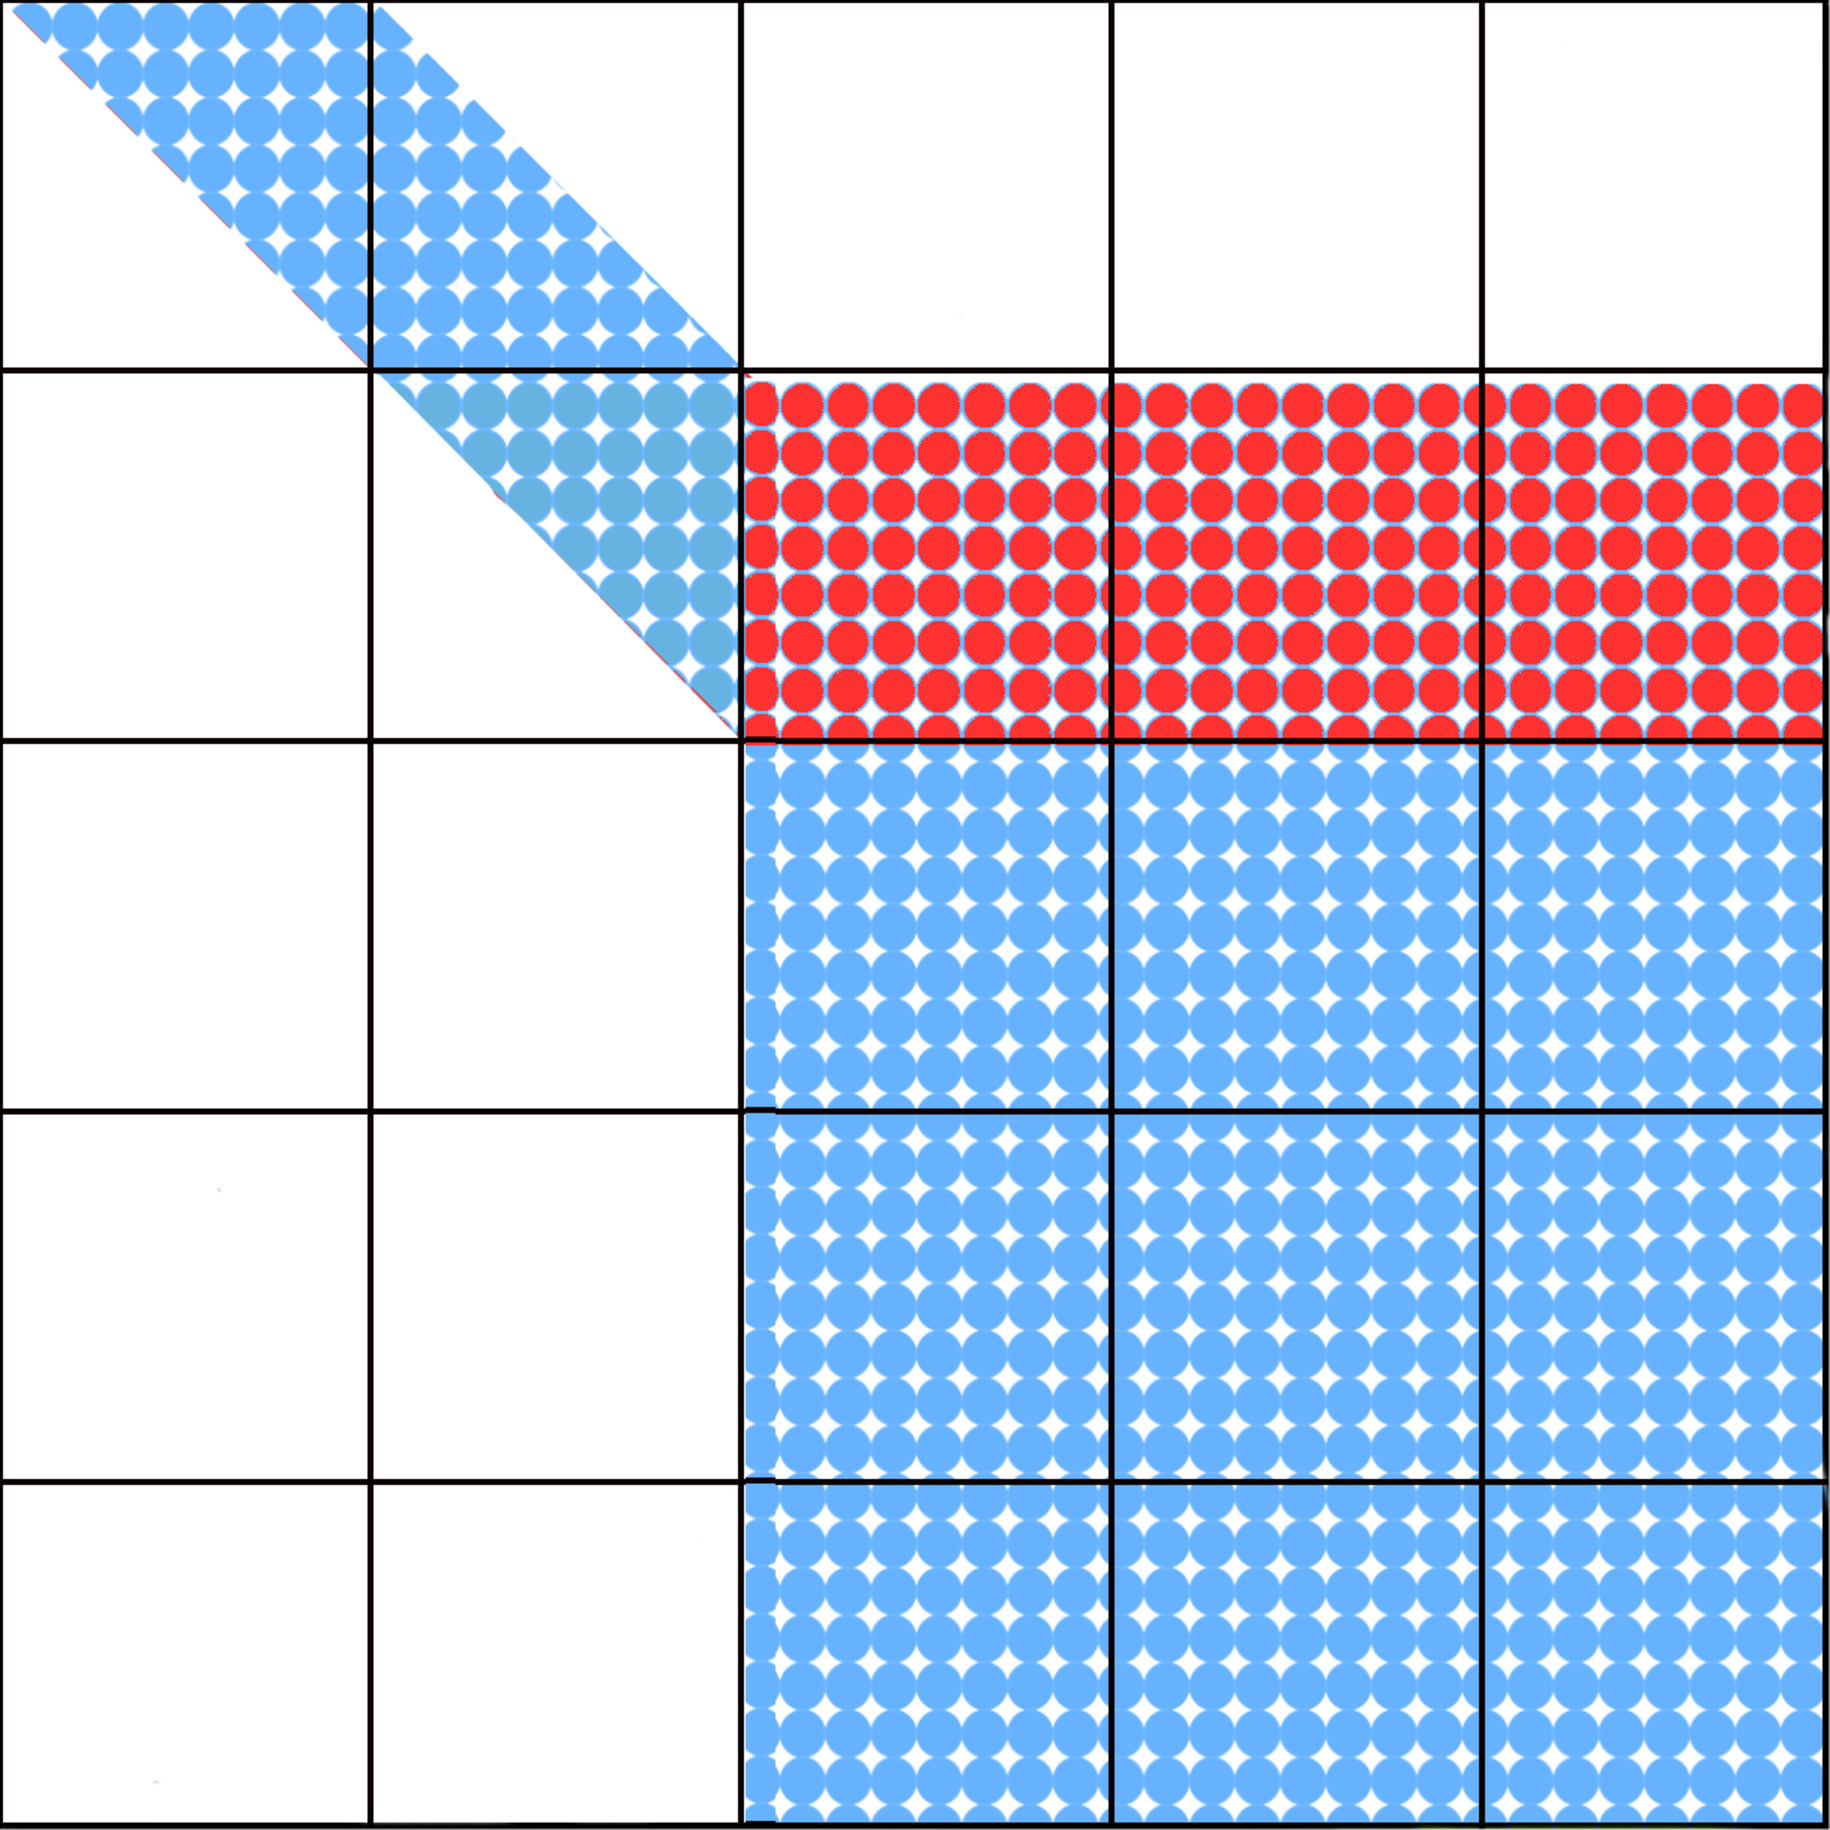
\includegraphics[width=\textwidth]{fig/SVD_panel_7_grid}
      \caption{\label{fig:lq_2}Row-tile LQ}
    \end{subfigure}
    \hfill
    %%%% 8
    \begin{subfigure}[t]{0.2 \textwidth}
      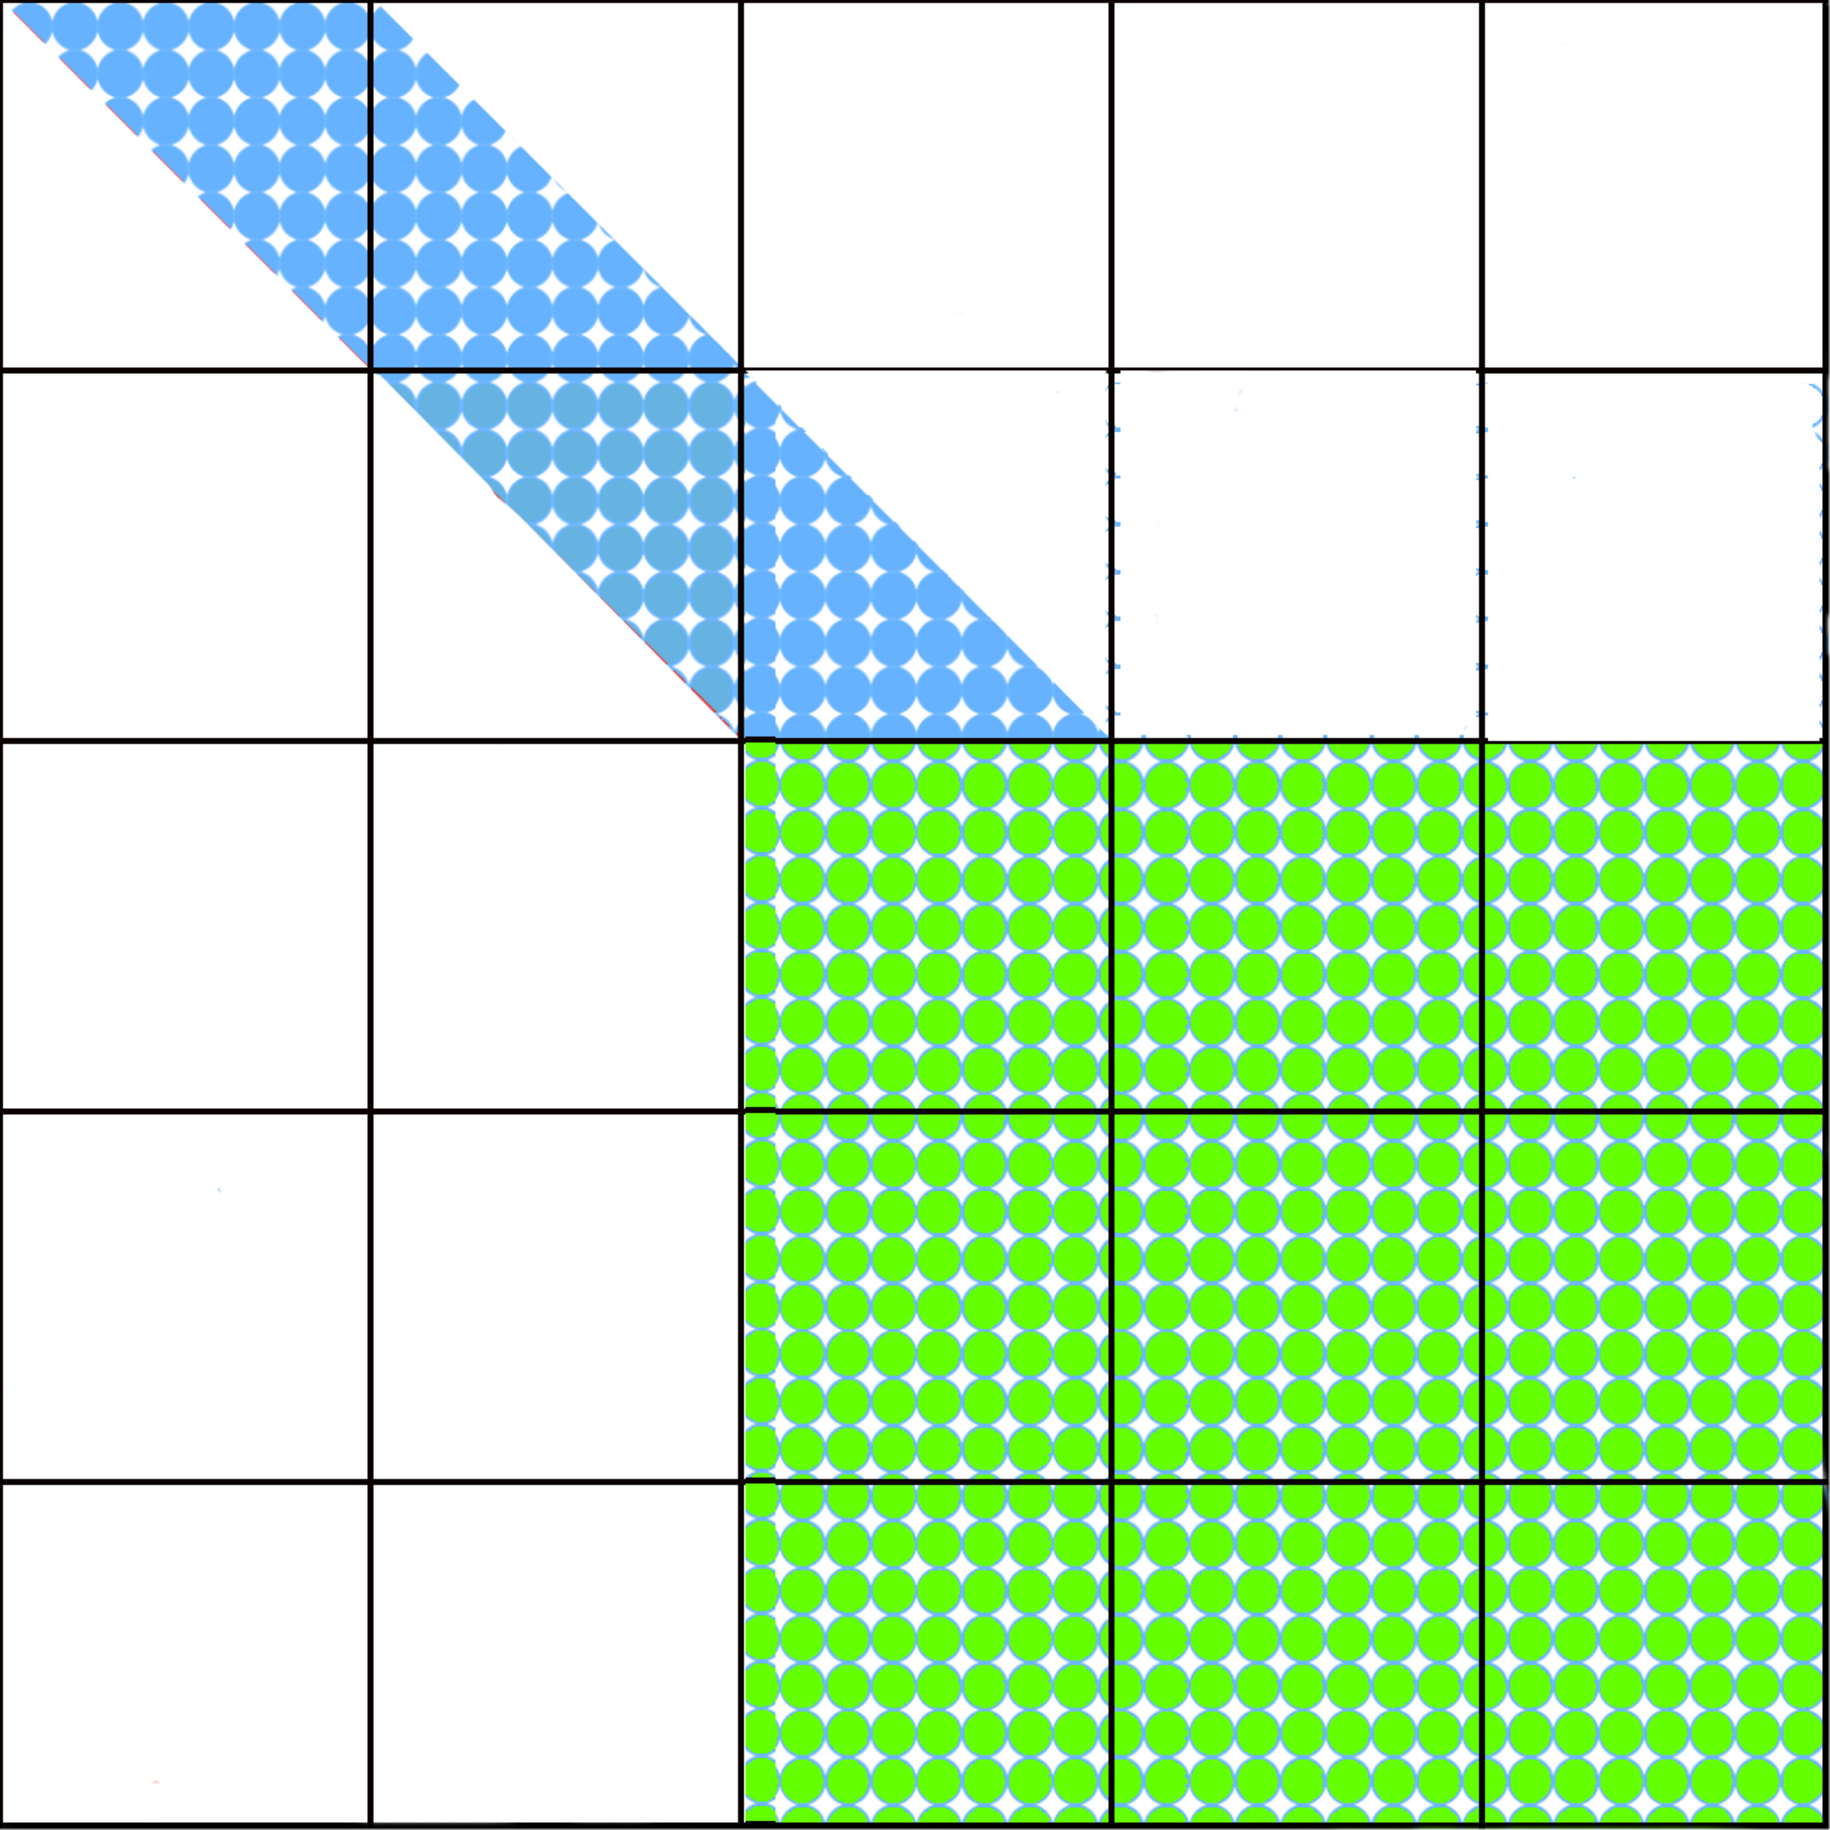
\includegraphics[width=\textwidth]{fig/SVD_panel_8_grid}
      \caption{\label{fig:lq_update_2}Update}
    \end{subfigure}
    \caption{Reduction from general matrix to band bidiagonal form
      using the late update strategy.
    \label{fig:panel}}
\end{figure}

The main advantage of this strategy is its simplicity,
the algorithm is very close to the LAPACK version. However the
individual steps of the QR factorization illustrated in
Figure~\ref{fig:rect_panel},
shows that a full factorization of a panel
starts with the $QR$ factorization of the first tile
(Figure~\ref{fig:geqrt_1}), which means only one CPU core is busy
while the others remain idle. Once the first tile is factorized the
rest of work (to annihilate the tiles below using the TSQRT
kernel) can commence.
Since the elimination procedure modifies the entries of the
top triangular tile only one square tile can be eliminated at a time
to guarantee a correct result.
Put differently,
the panel factorization introduces synchronization points
in the algorithm that
may lead to performance penalties.
The sequential nature of the panel factorization can be
clearly observed in Figure~\ref{fig:dag_panel},
which shows the DAG of the corresponding operations.

\begin{figure}
  \begin{center}
    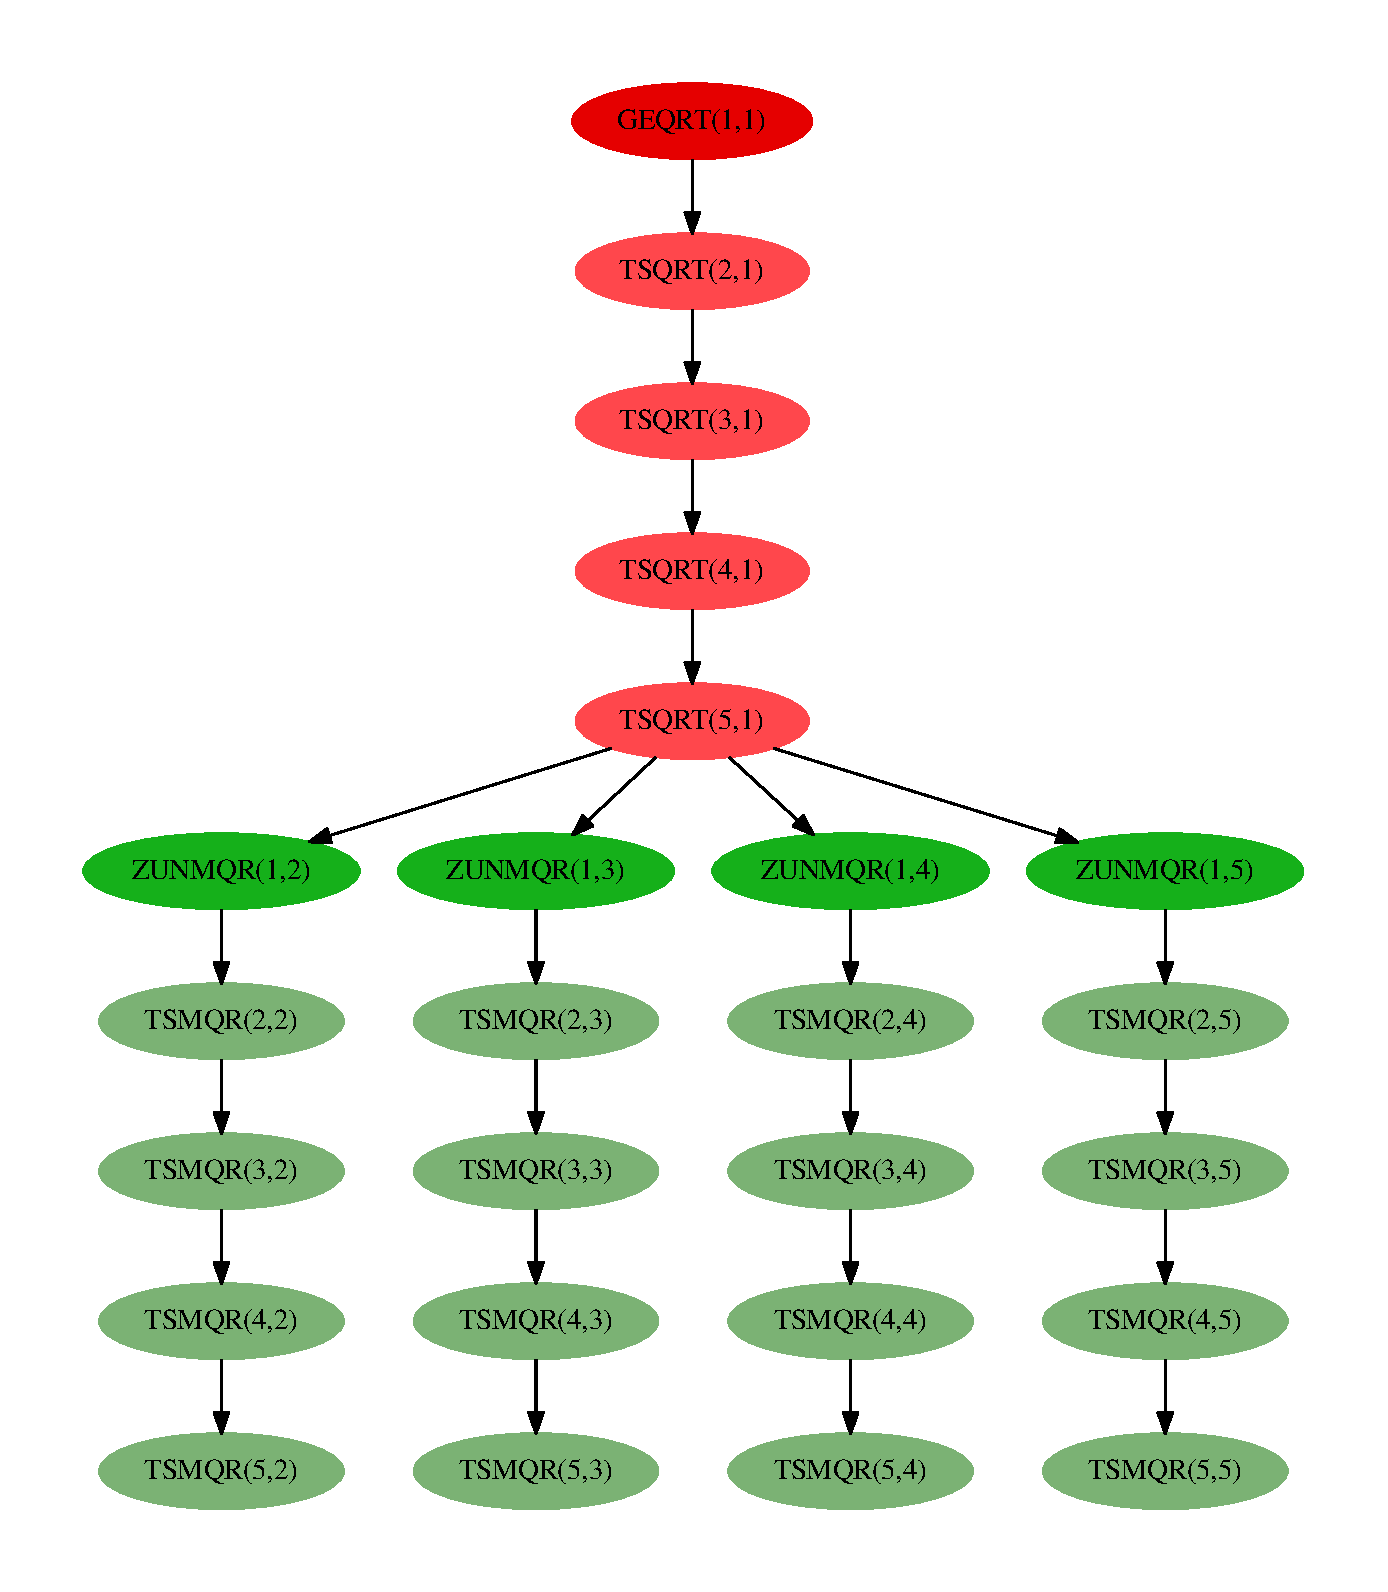
\includegraphics[width=0.5\textwidth]{fig/dag}
  \end{center}
  \caption{DAG of the late update strategy for band reduction:
    this partial view is limited to the factorization of the first panel and
    the update of the corresponding trailing matrix.}
  \label{fig:dag_panel}
\end{figure}

One can overcome this synchronization issue by overlapping the panel
factorization and the update steps.
The algorithm can then progress onto the next step even
though the previous step is not completed,
as long as we respect the data dependencies.
In addition, when working on a panel we can
take advantage of ``tall and skinny'' QR factorization
strategies:
providing elegant methods to introduce parallelism
during a panel factorization.
This leads us to the early update strategy.

\subsection{Early update strategy}
To reduce a full tile matrix to a band bidiagonal form,
the early update strategy also completes the QR factorization
of the first panel and the update before starting the LQ process,
but the operations are launched in a completely different order.
Instead of completing the full factorization of a panel
before applying the updates as before,
the early update strategy looks down the panel,
factorizes each tile, and then launches
its corresponding updates immediately.

As depicted in Figure~\ref{fig:tile}, the algorithm starts with the
factorization of the tile $A(1,1)$ (Figure~\ref{fig:tile_qr_1}),
before applying the corresponding transformations to the rest of the
tile-row (Figure~\ref{fig:tile_qr_update_1}).
Once the first tile is factorized
the remaining tiles in the panel are successively eliminated
and, in the same way, the trailing submatrices are updated immediately
(as illustrated in Figures~\ref{fig:tile_qr_2}
and~\ref{fig:tile_qr_update_2}
as well as in Figures~\ref{fig:tile_qr_3}
and~\ref{fig:tile_qr_update_3}).
In addition,
the updates in Figure~\ref{fig:tile_qr_update_2} can be computed in parallel
with the next tile elimination in Figure~\ref{fig:tile_qr_3}.
The same approach is used during the LQ factorization step.

\begin{figure}[h!]
  %%%% 1
  \begin{subfigure}{0.2 \textwidth}
    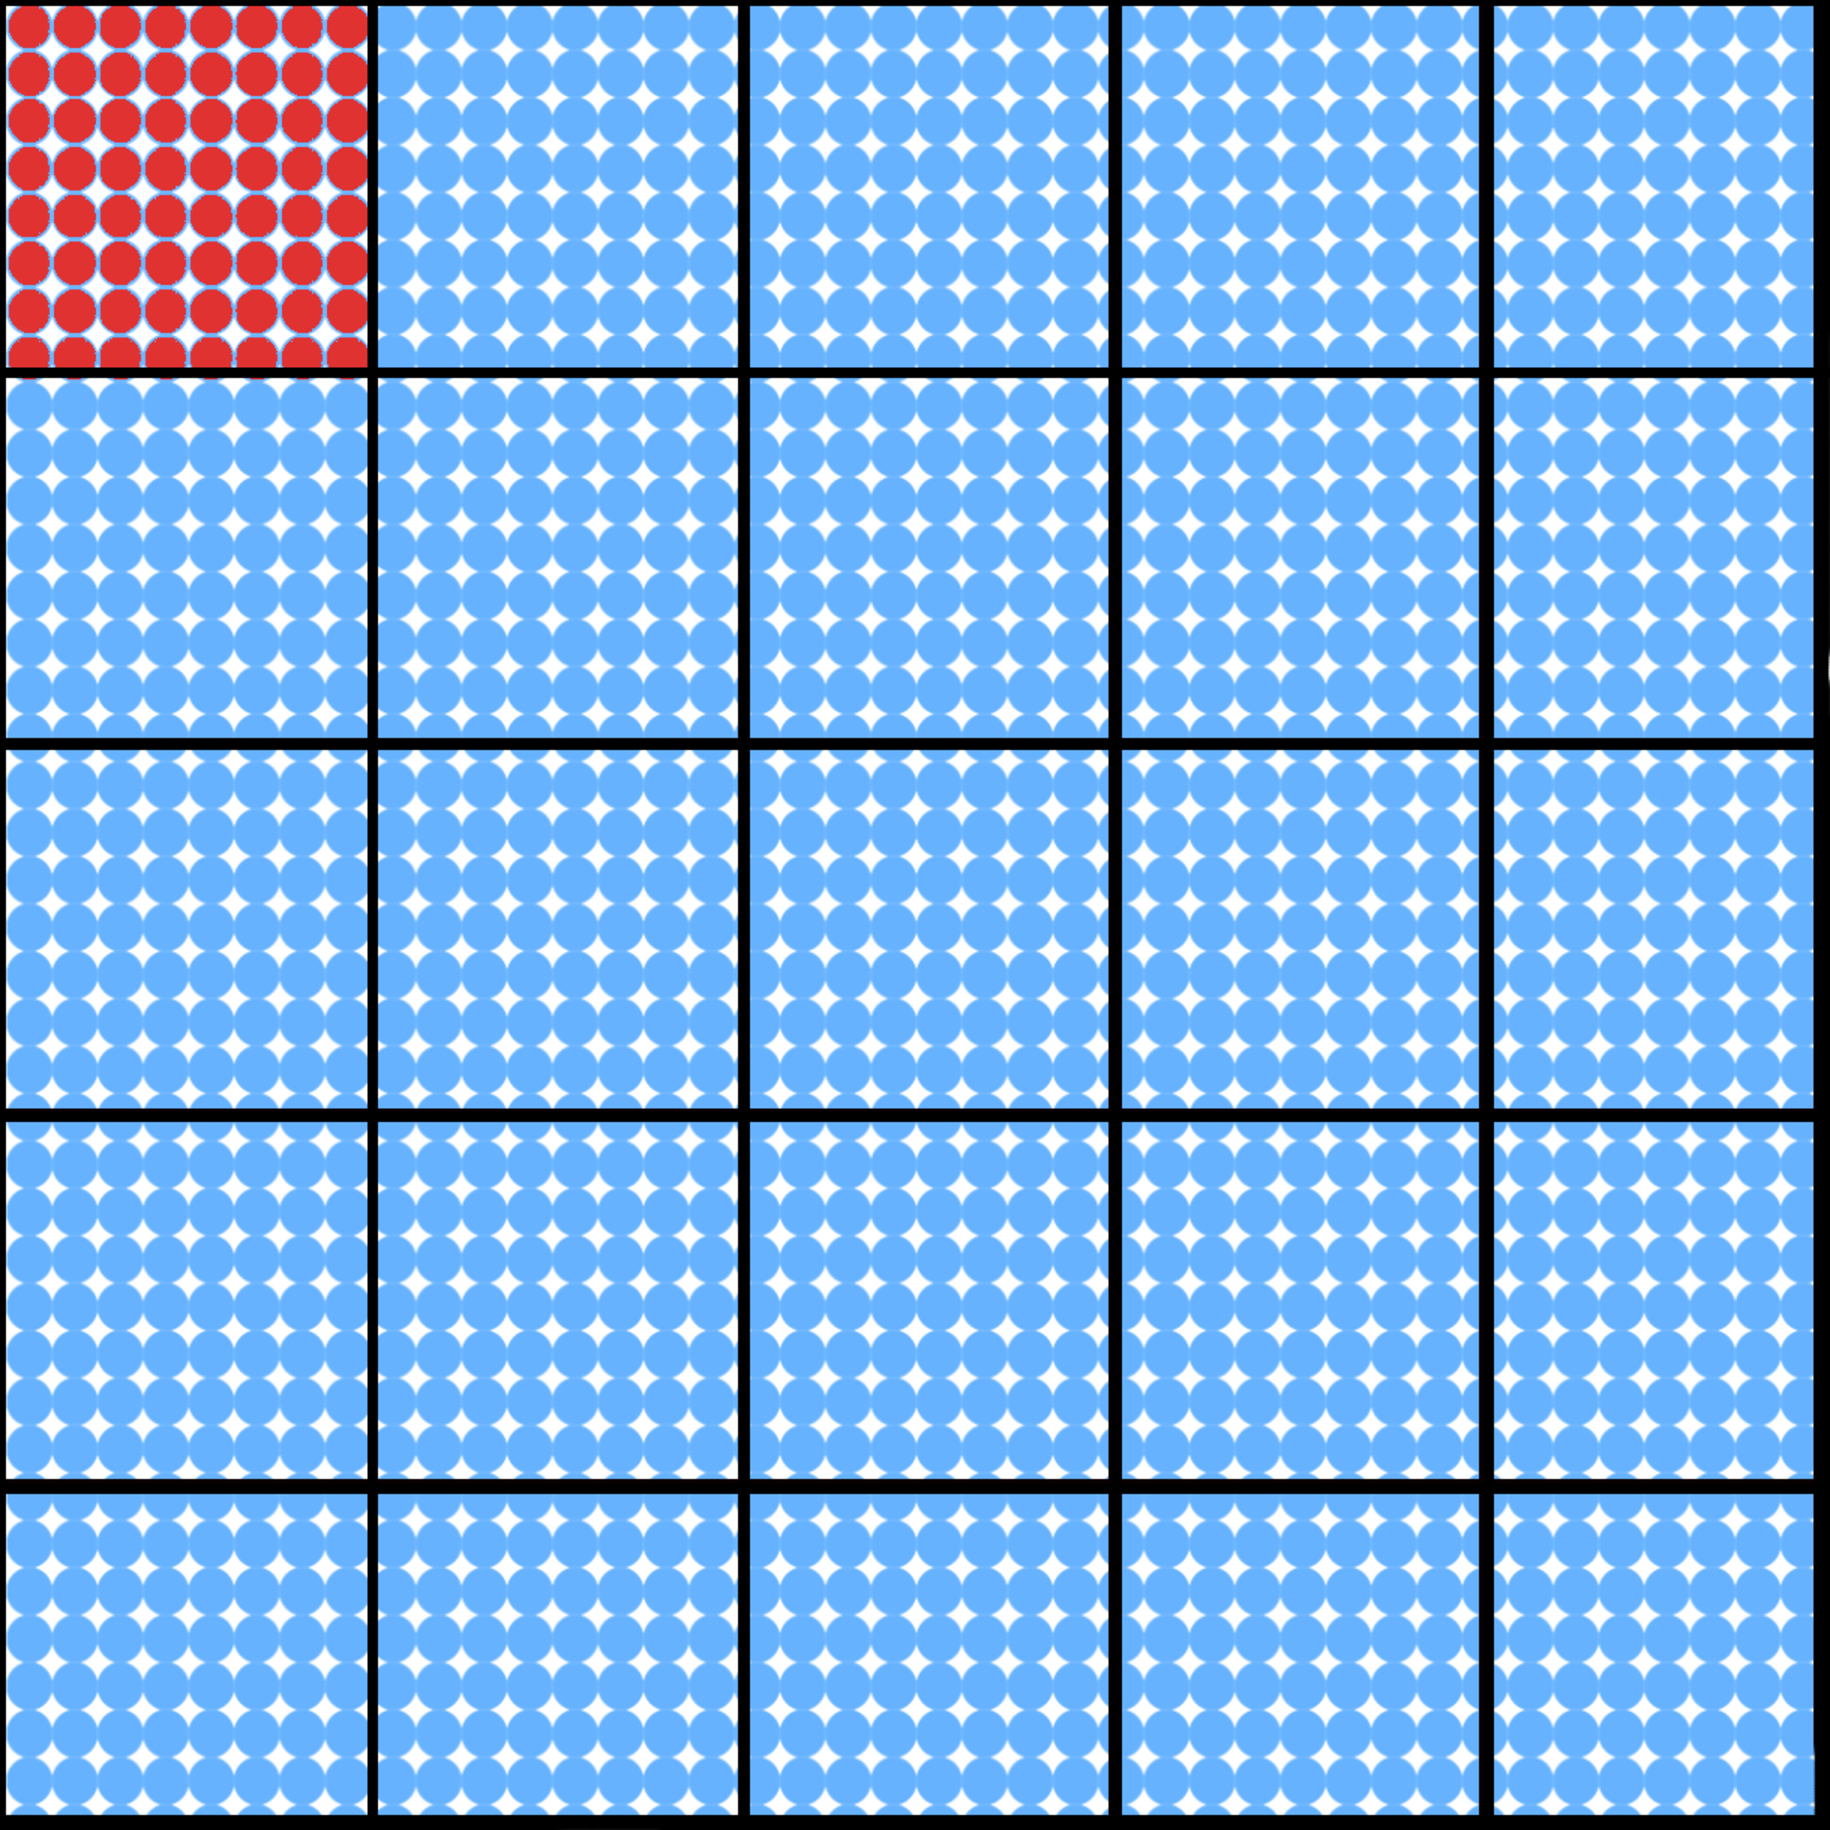
\includegraphics[width=\textwidth]{fig/SVD_tile_1_grid}
    \caption{\label{fig:tile_qr_1} Top corner QR}
  \end{subfigure}
  \hfill
  %%%% 2
  \begin{subfigure}{0.2 \textwidth}
    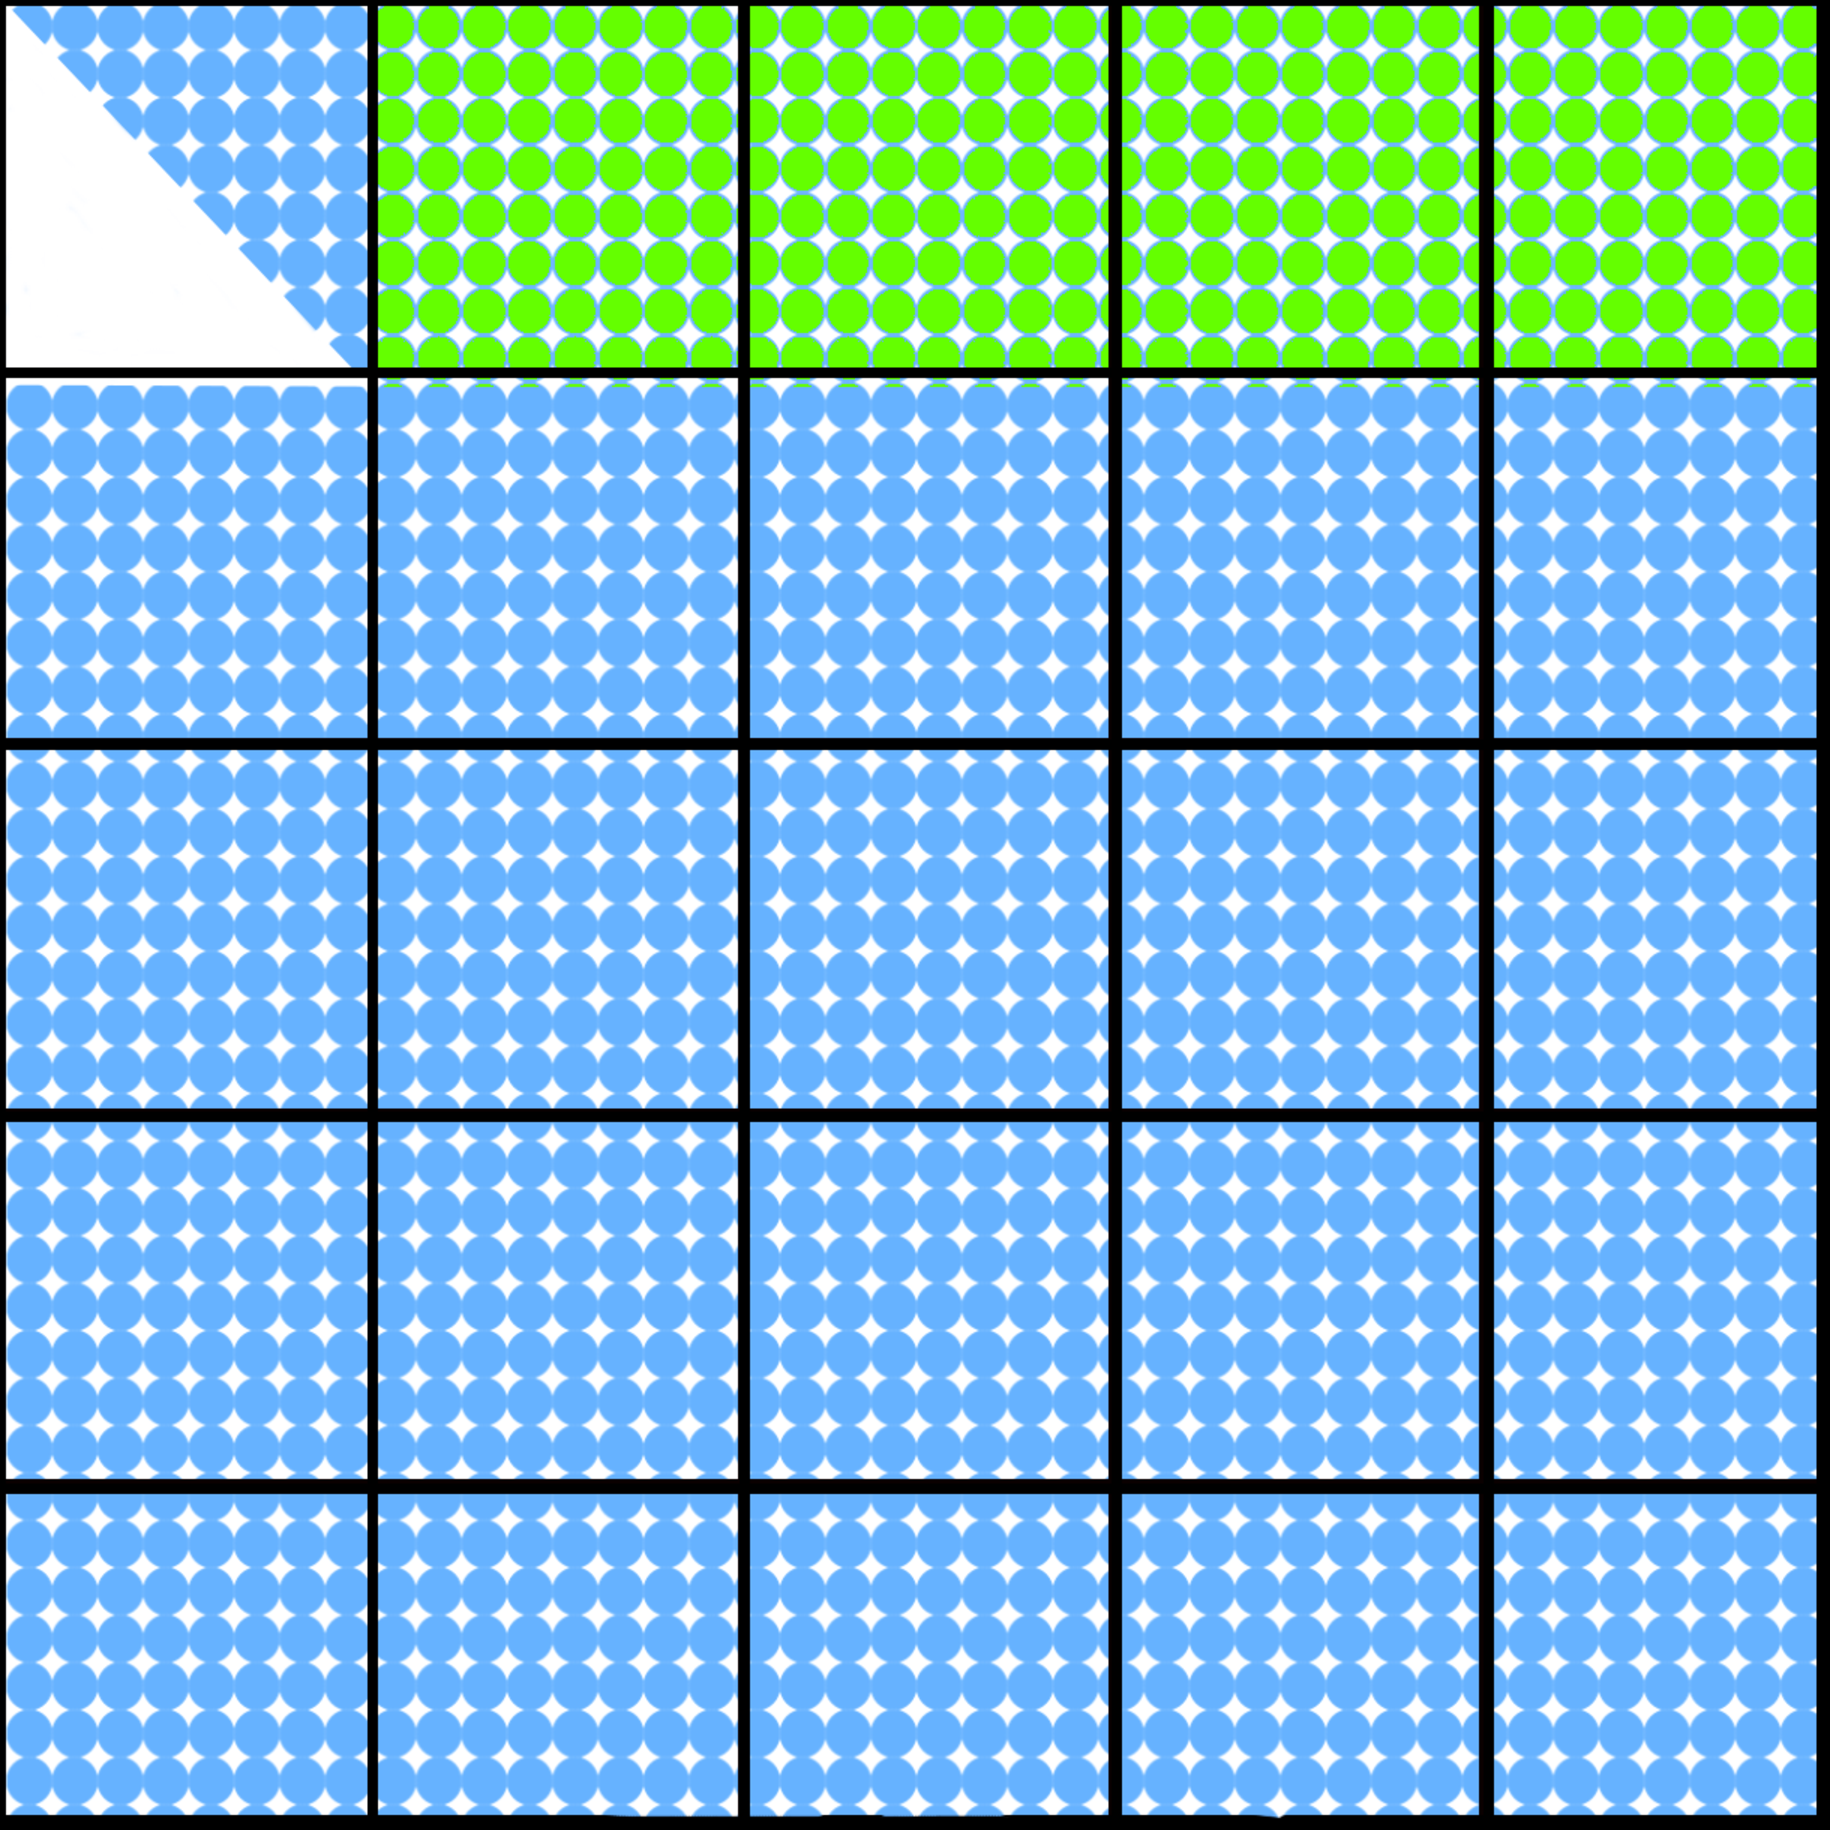
\includegraphics[width=\textwidth]{fig/SVD_tile_2_grid}
    \caption{\label{fig:tile_qr_update_1}Tile-row update}
  \end{subfigure}
  \hfill
  %%%% 3
  \begin{subfigure}{0.2 \textwidth}
    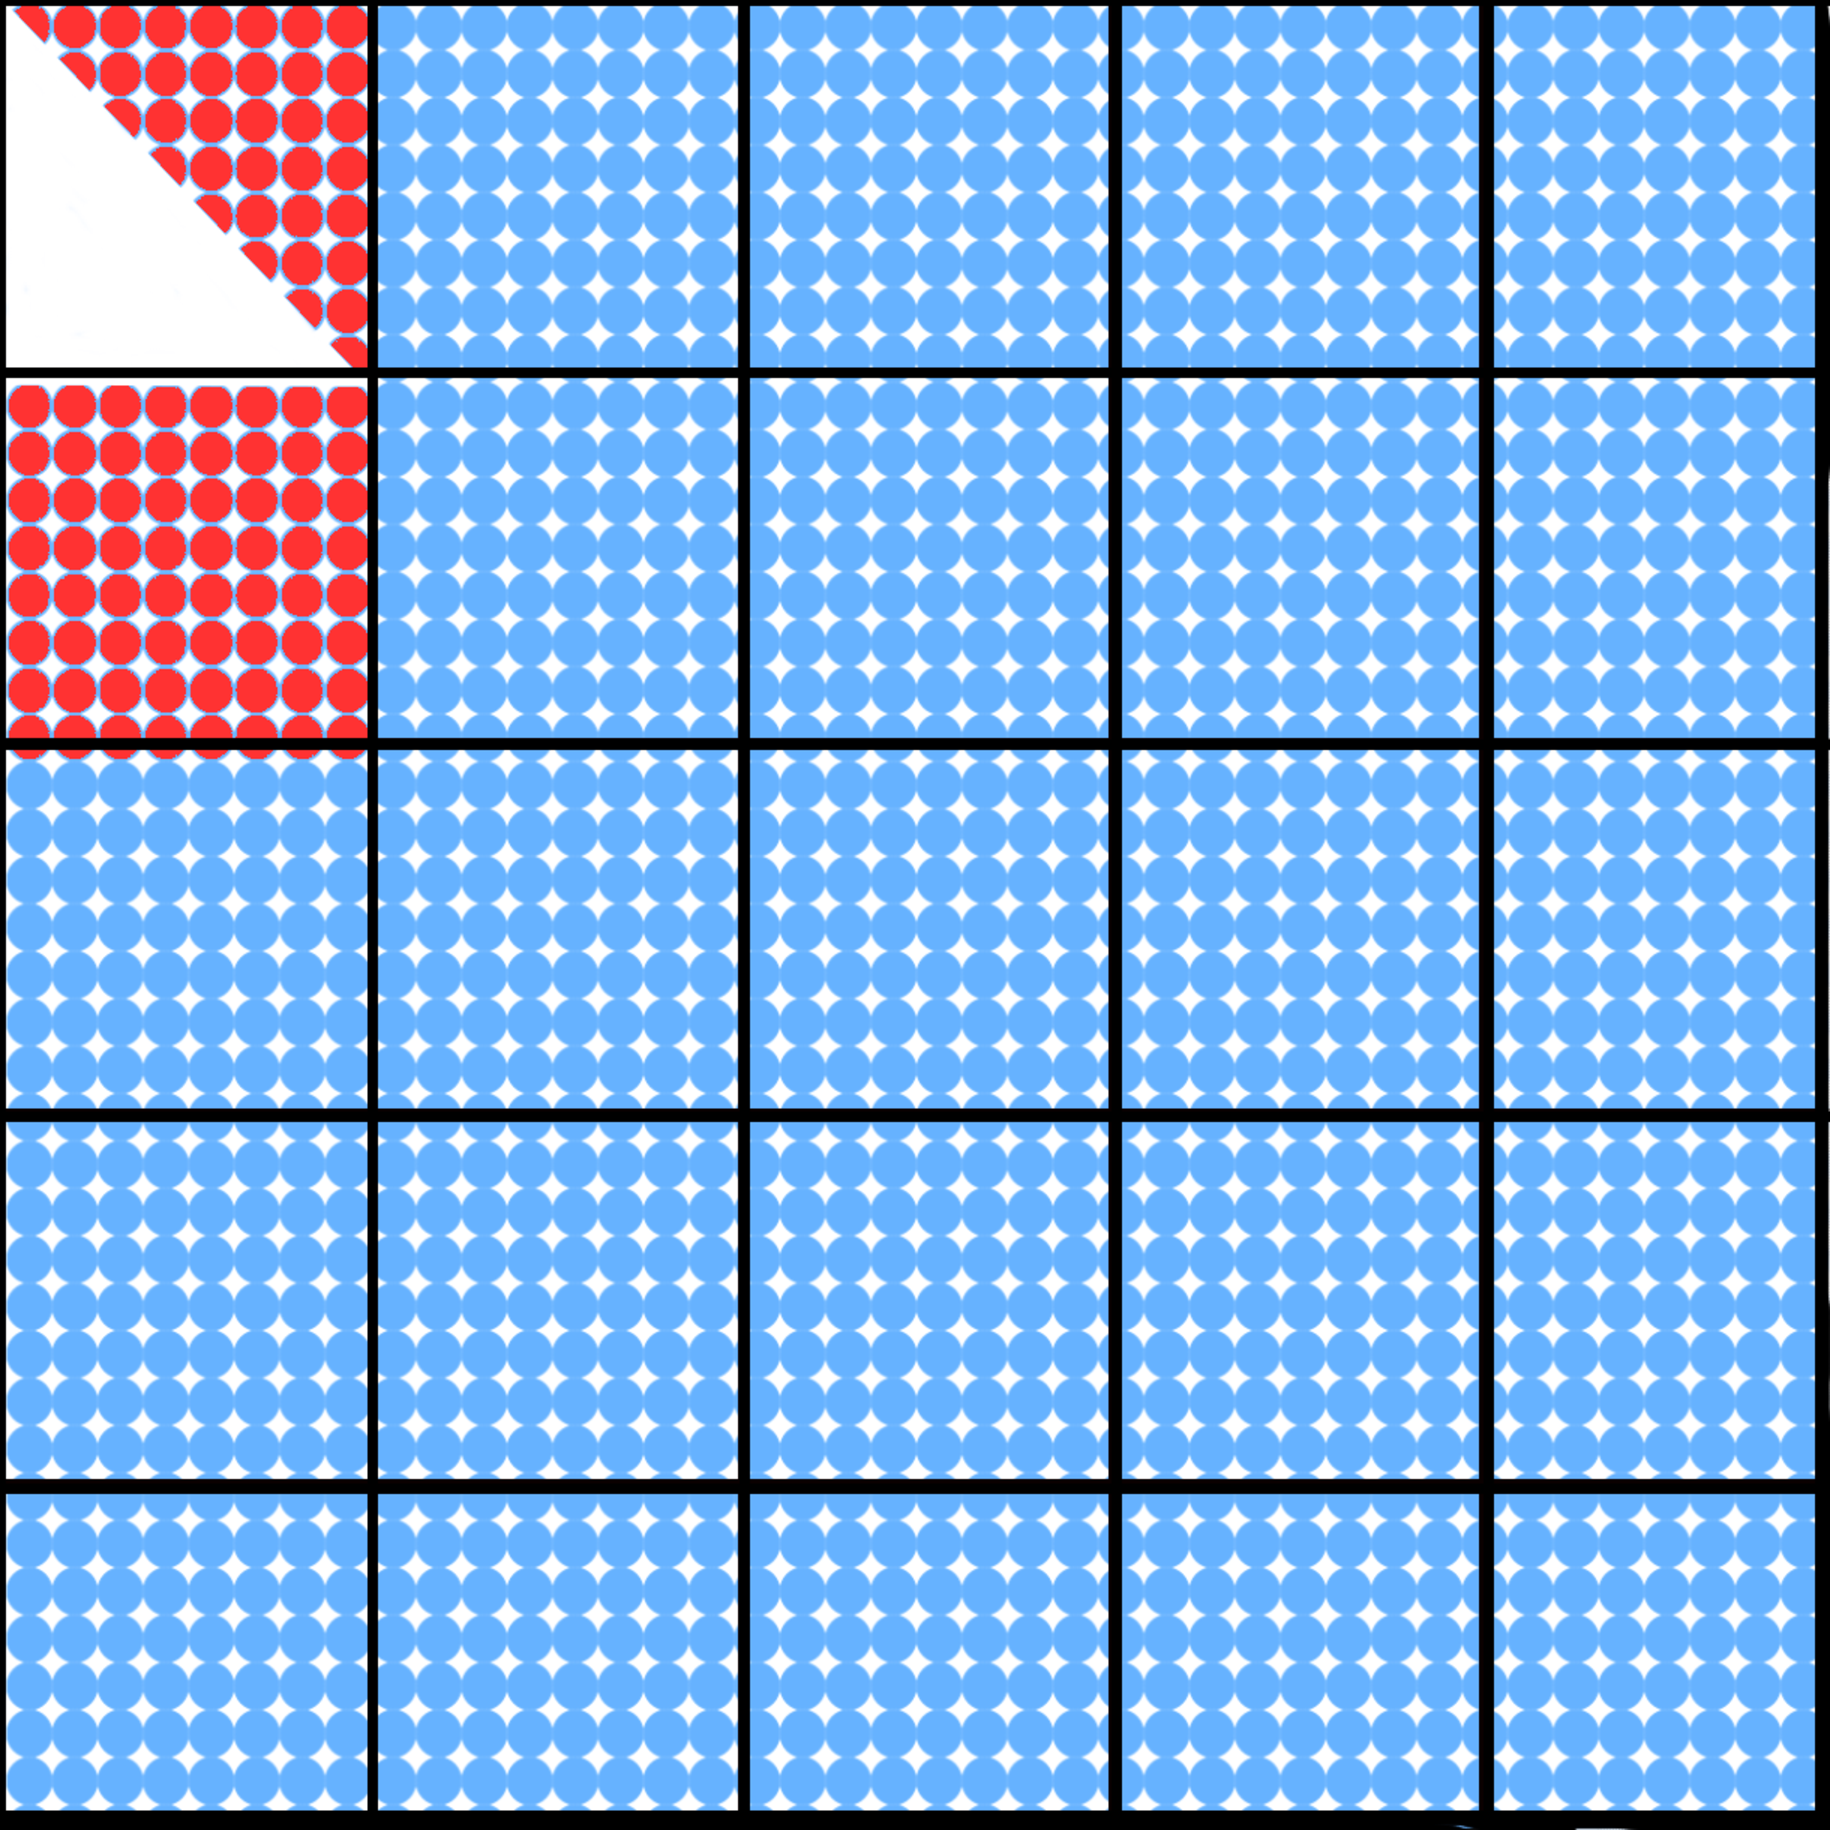
\includegraphics[width=\textwidth]{fig/SVD_tile_3_grid}
    \caption{\label{fig:tile_qr_2}TSQRT}
  \end{subfigure}
  \hfill
  %%%% 4
  \begin{subfigure}{0.2 \textwidth}
    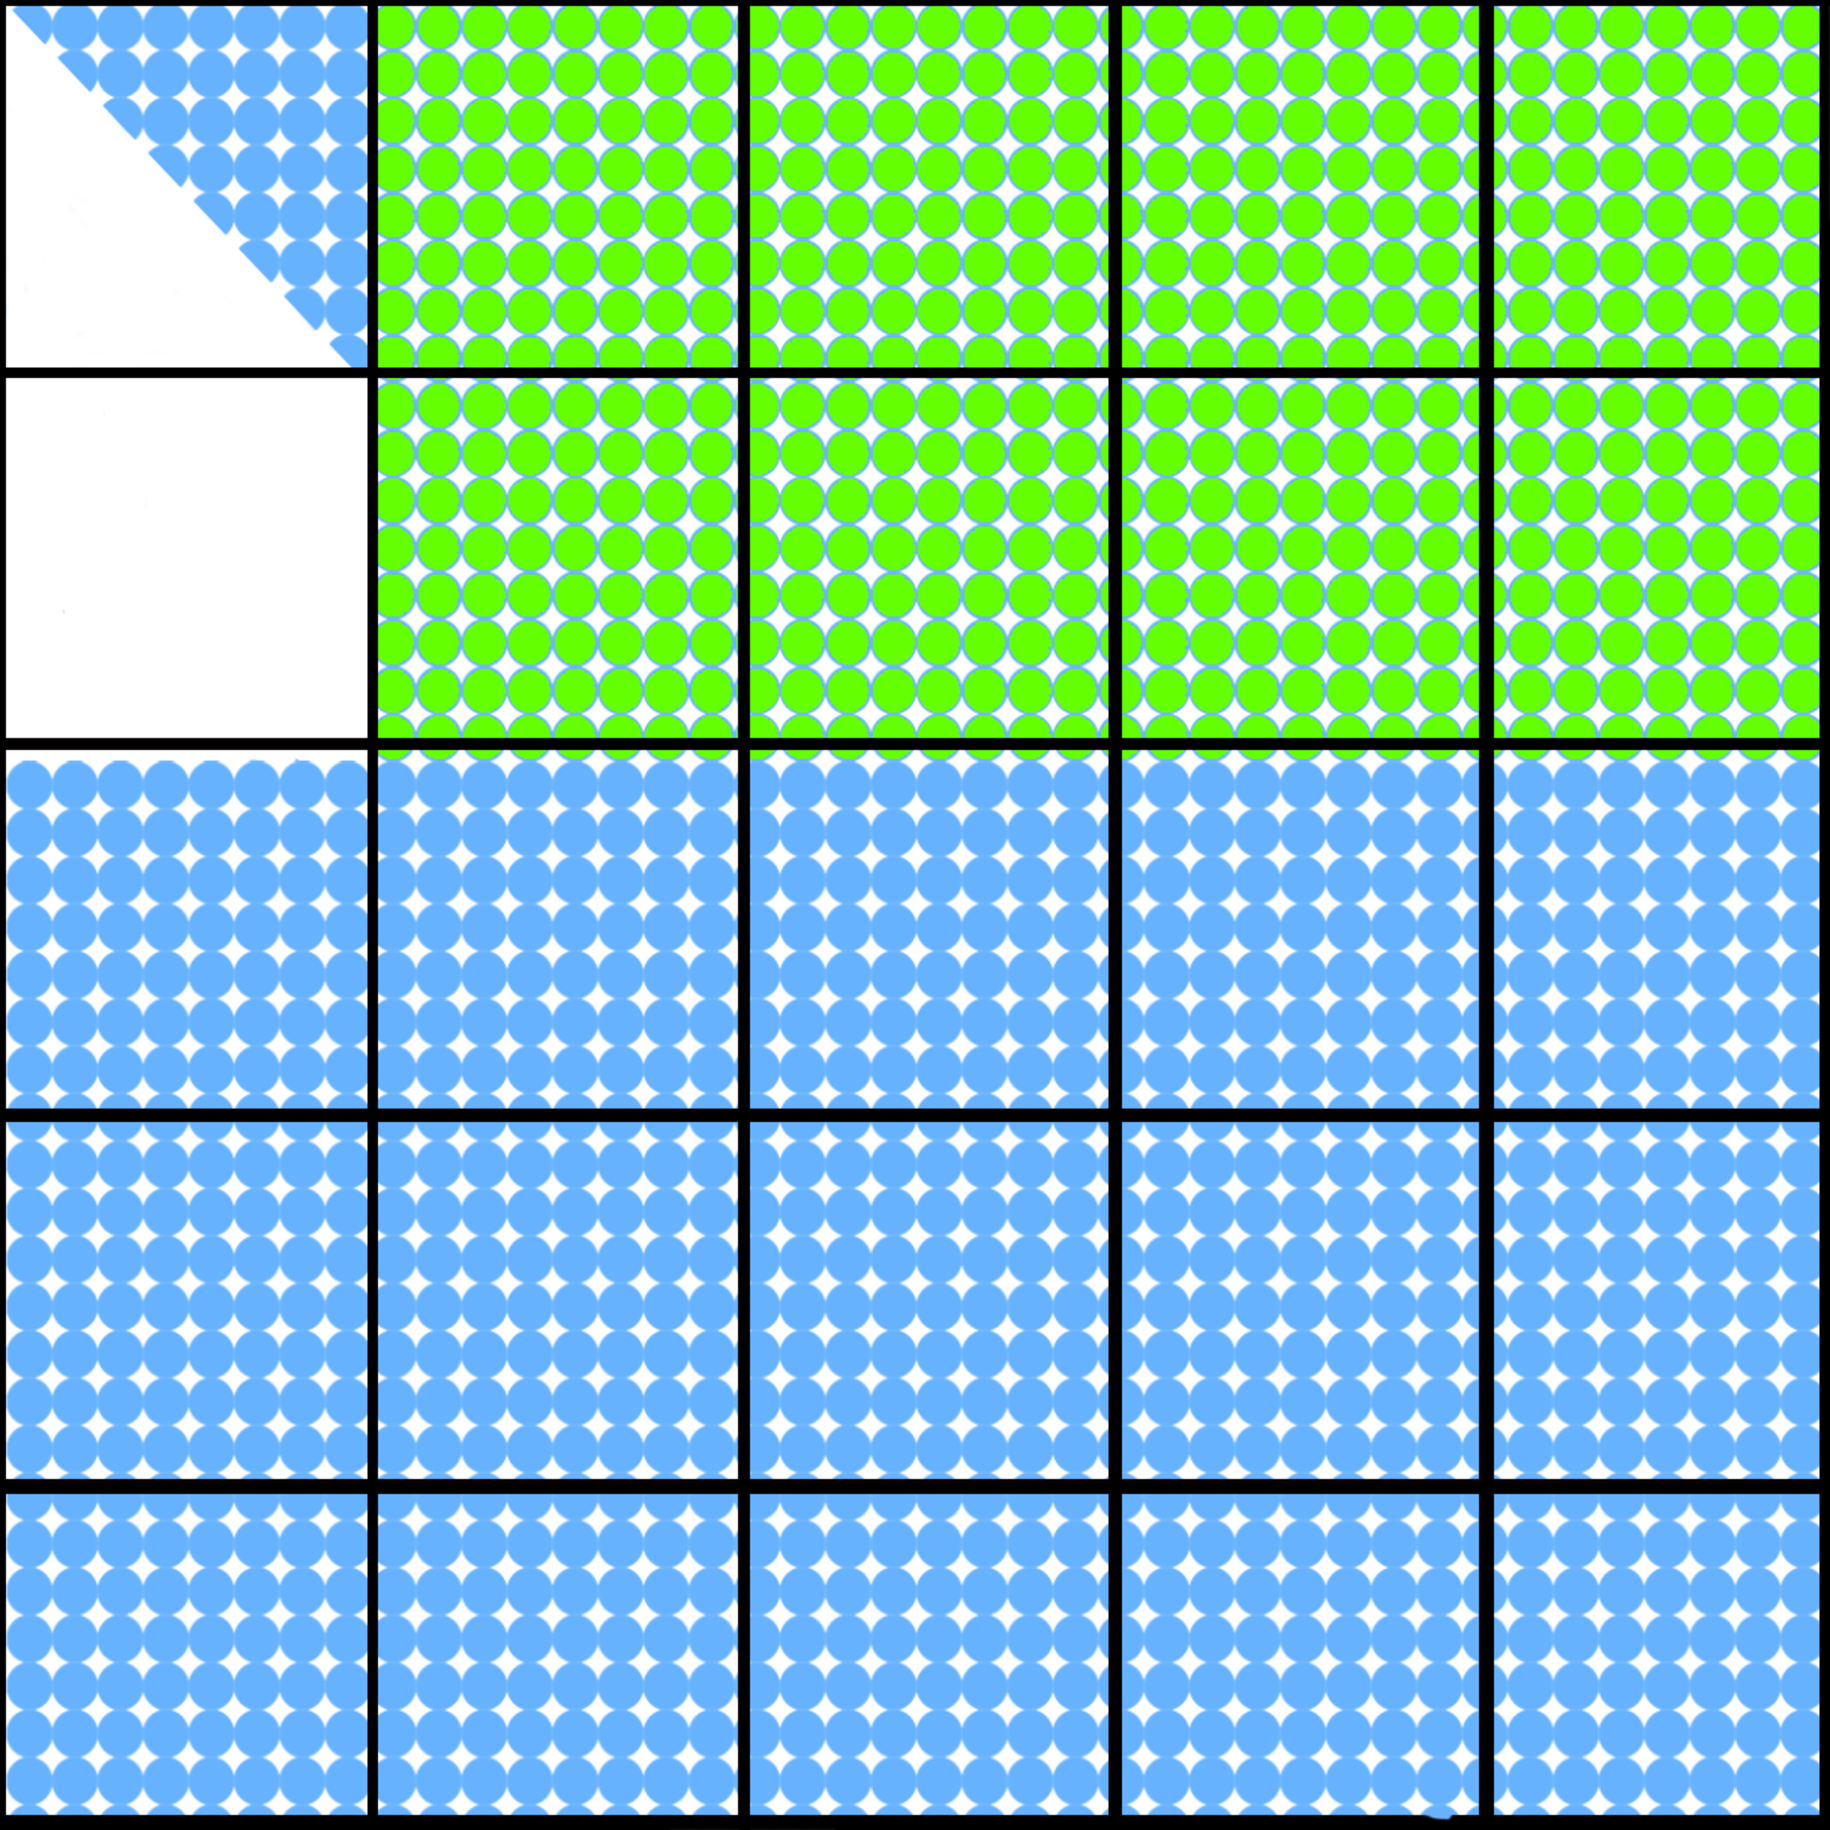
\includegraphics[width=\textwidth]{fig/SVD_tile_4_grid}
    \caption{\label{fig:tile_qr_update_2}Tile-rows update}
  \end{subfigure}
  \hfill
  %%%% 5
  \begin{subfigure}{0.2 \textwidth}
    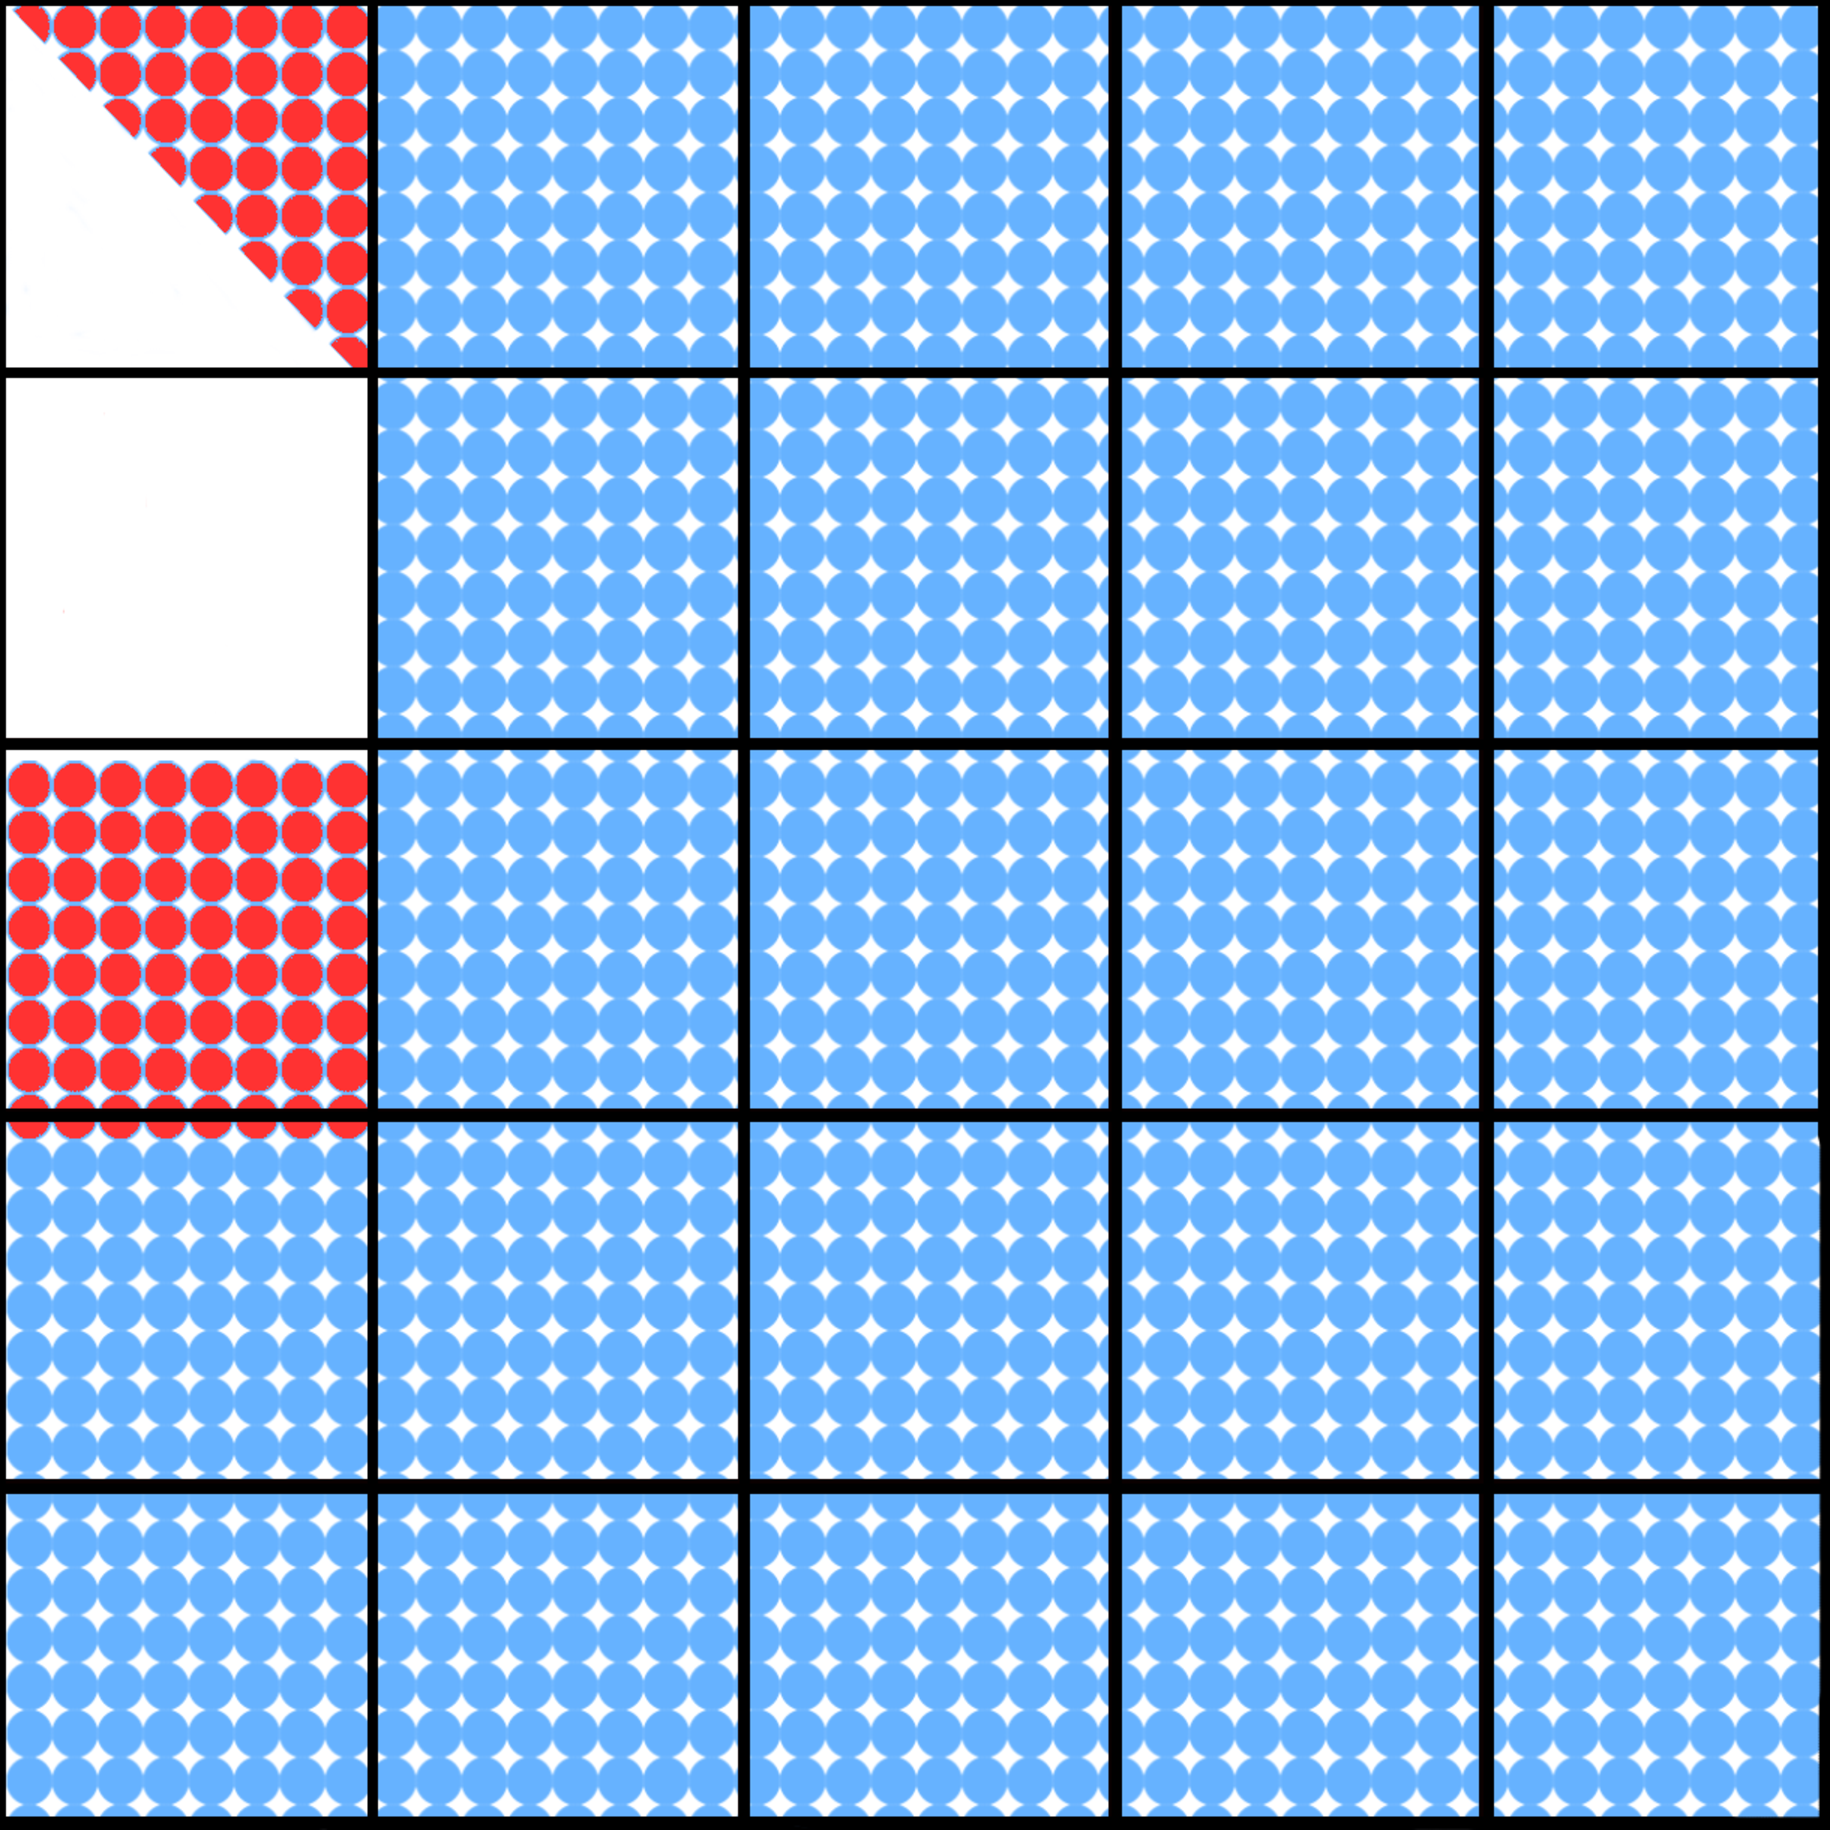
\includegraphics[width=\textwidth]{fig/SVD_tile_5_grid}
    \caption{\label{fig:tile_qr_3}TSQRT}
  \end{subfigure}
  \hfill
  %%%% 6
  \begin{subfigure}{0.2 \textwidth}
    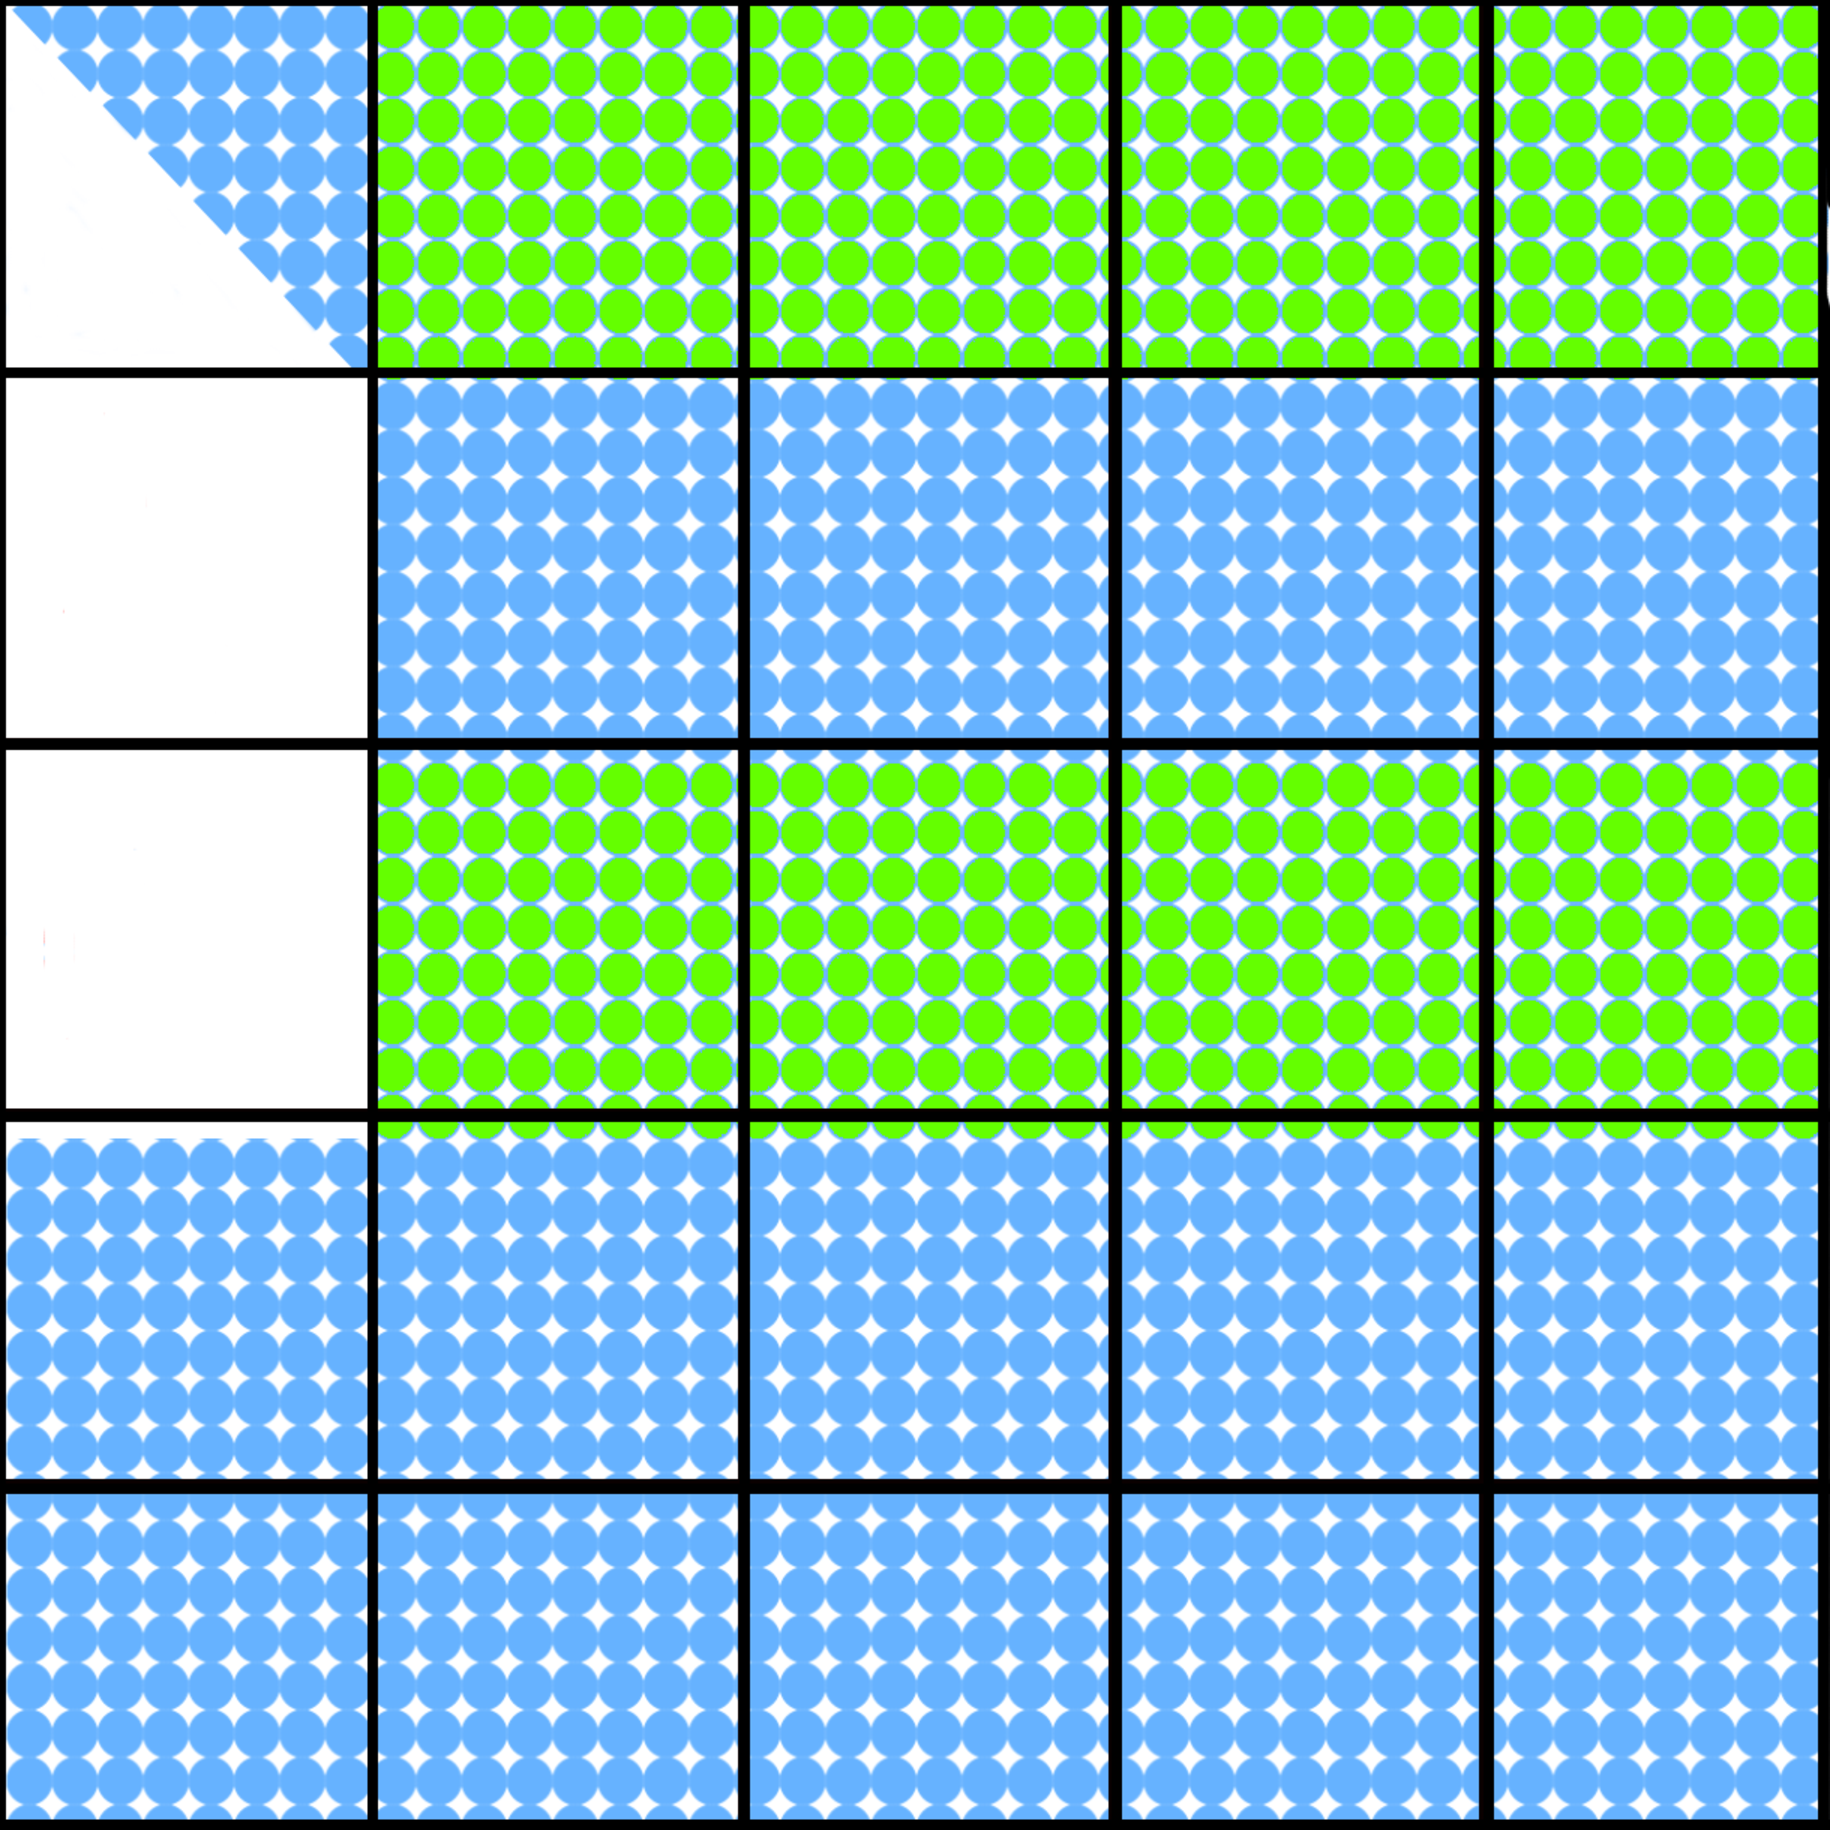
\includegraphics[width=\textwidth]{fig/SVD_tile_6_grid}
    \caption{\label{fig:tile_qr_update_3}Tile-rows update}
  \end{subfigure}
  \hfill
  %%%% 7
  \begin{subfigure}{0.2 \textwidth}
    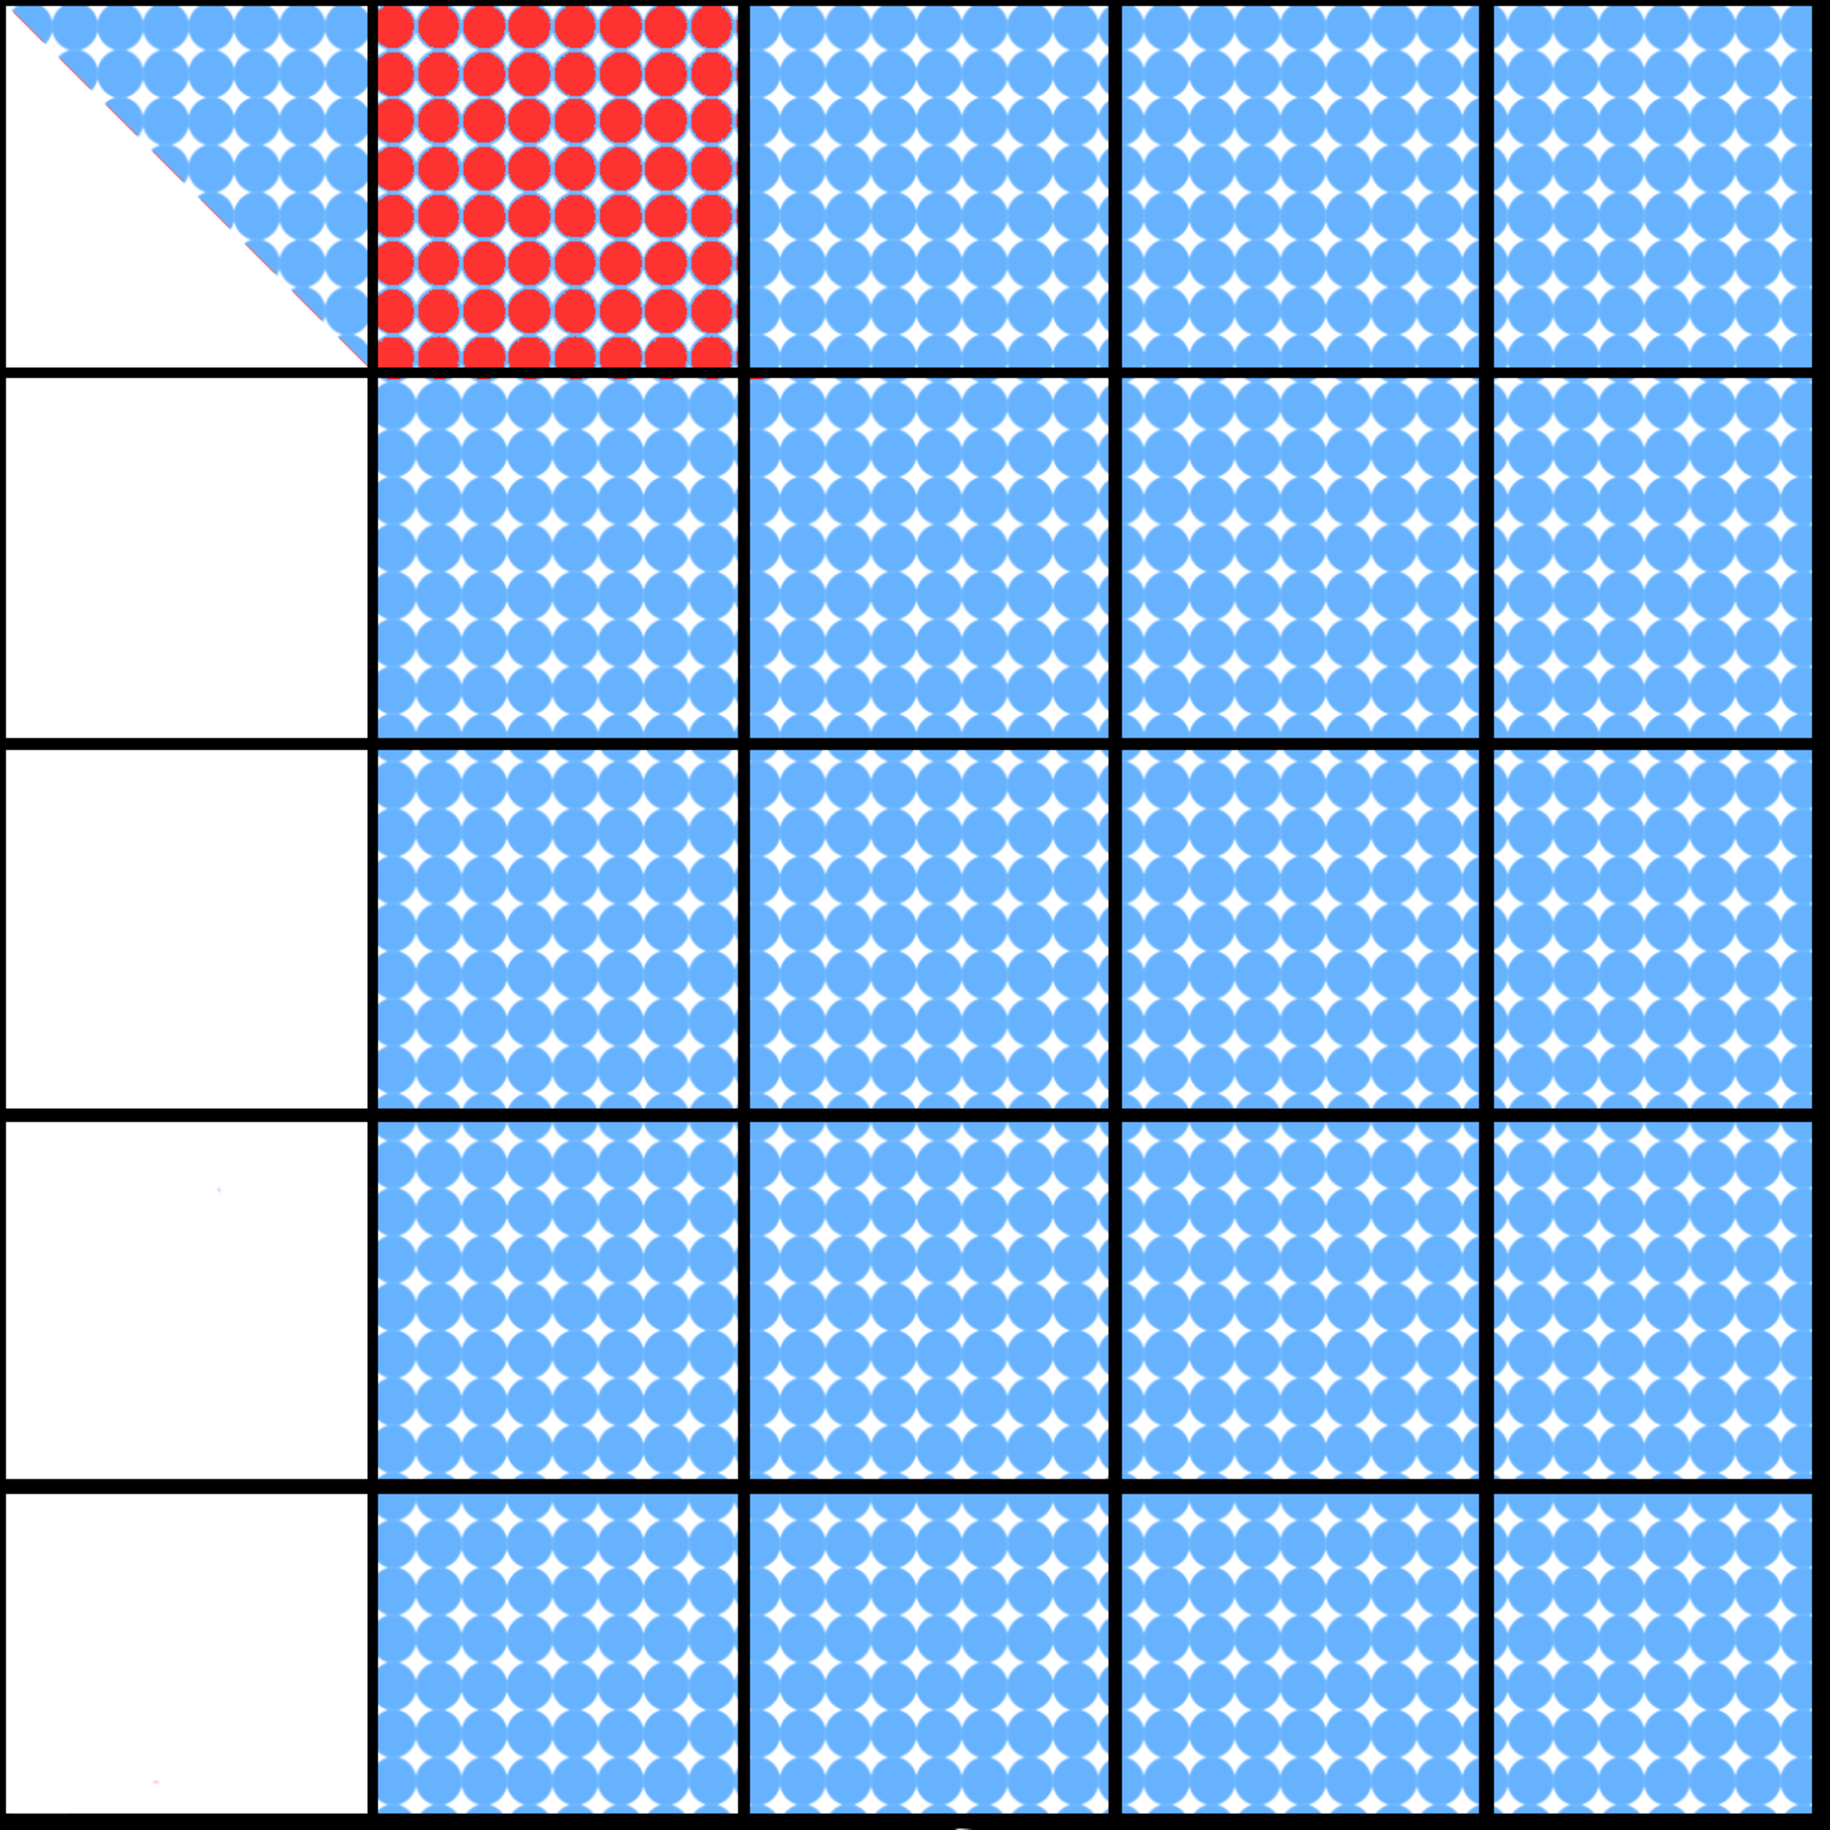
\includegraphics[width=\textwidth]{fig/SVD_tile_7_grid}
      \caption{\label{fig:tile_lq_2}LQ }
  \end{subfigure}
  \hfill
  %%%% 8
  \begin{subfigure}{0.2 \textwidth}
    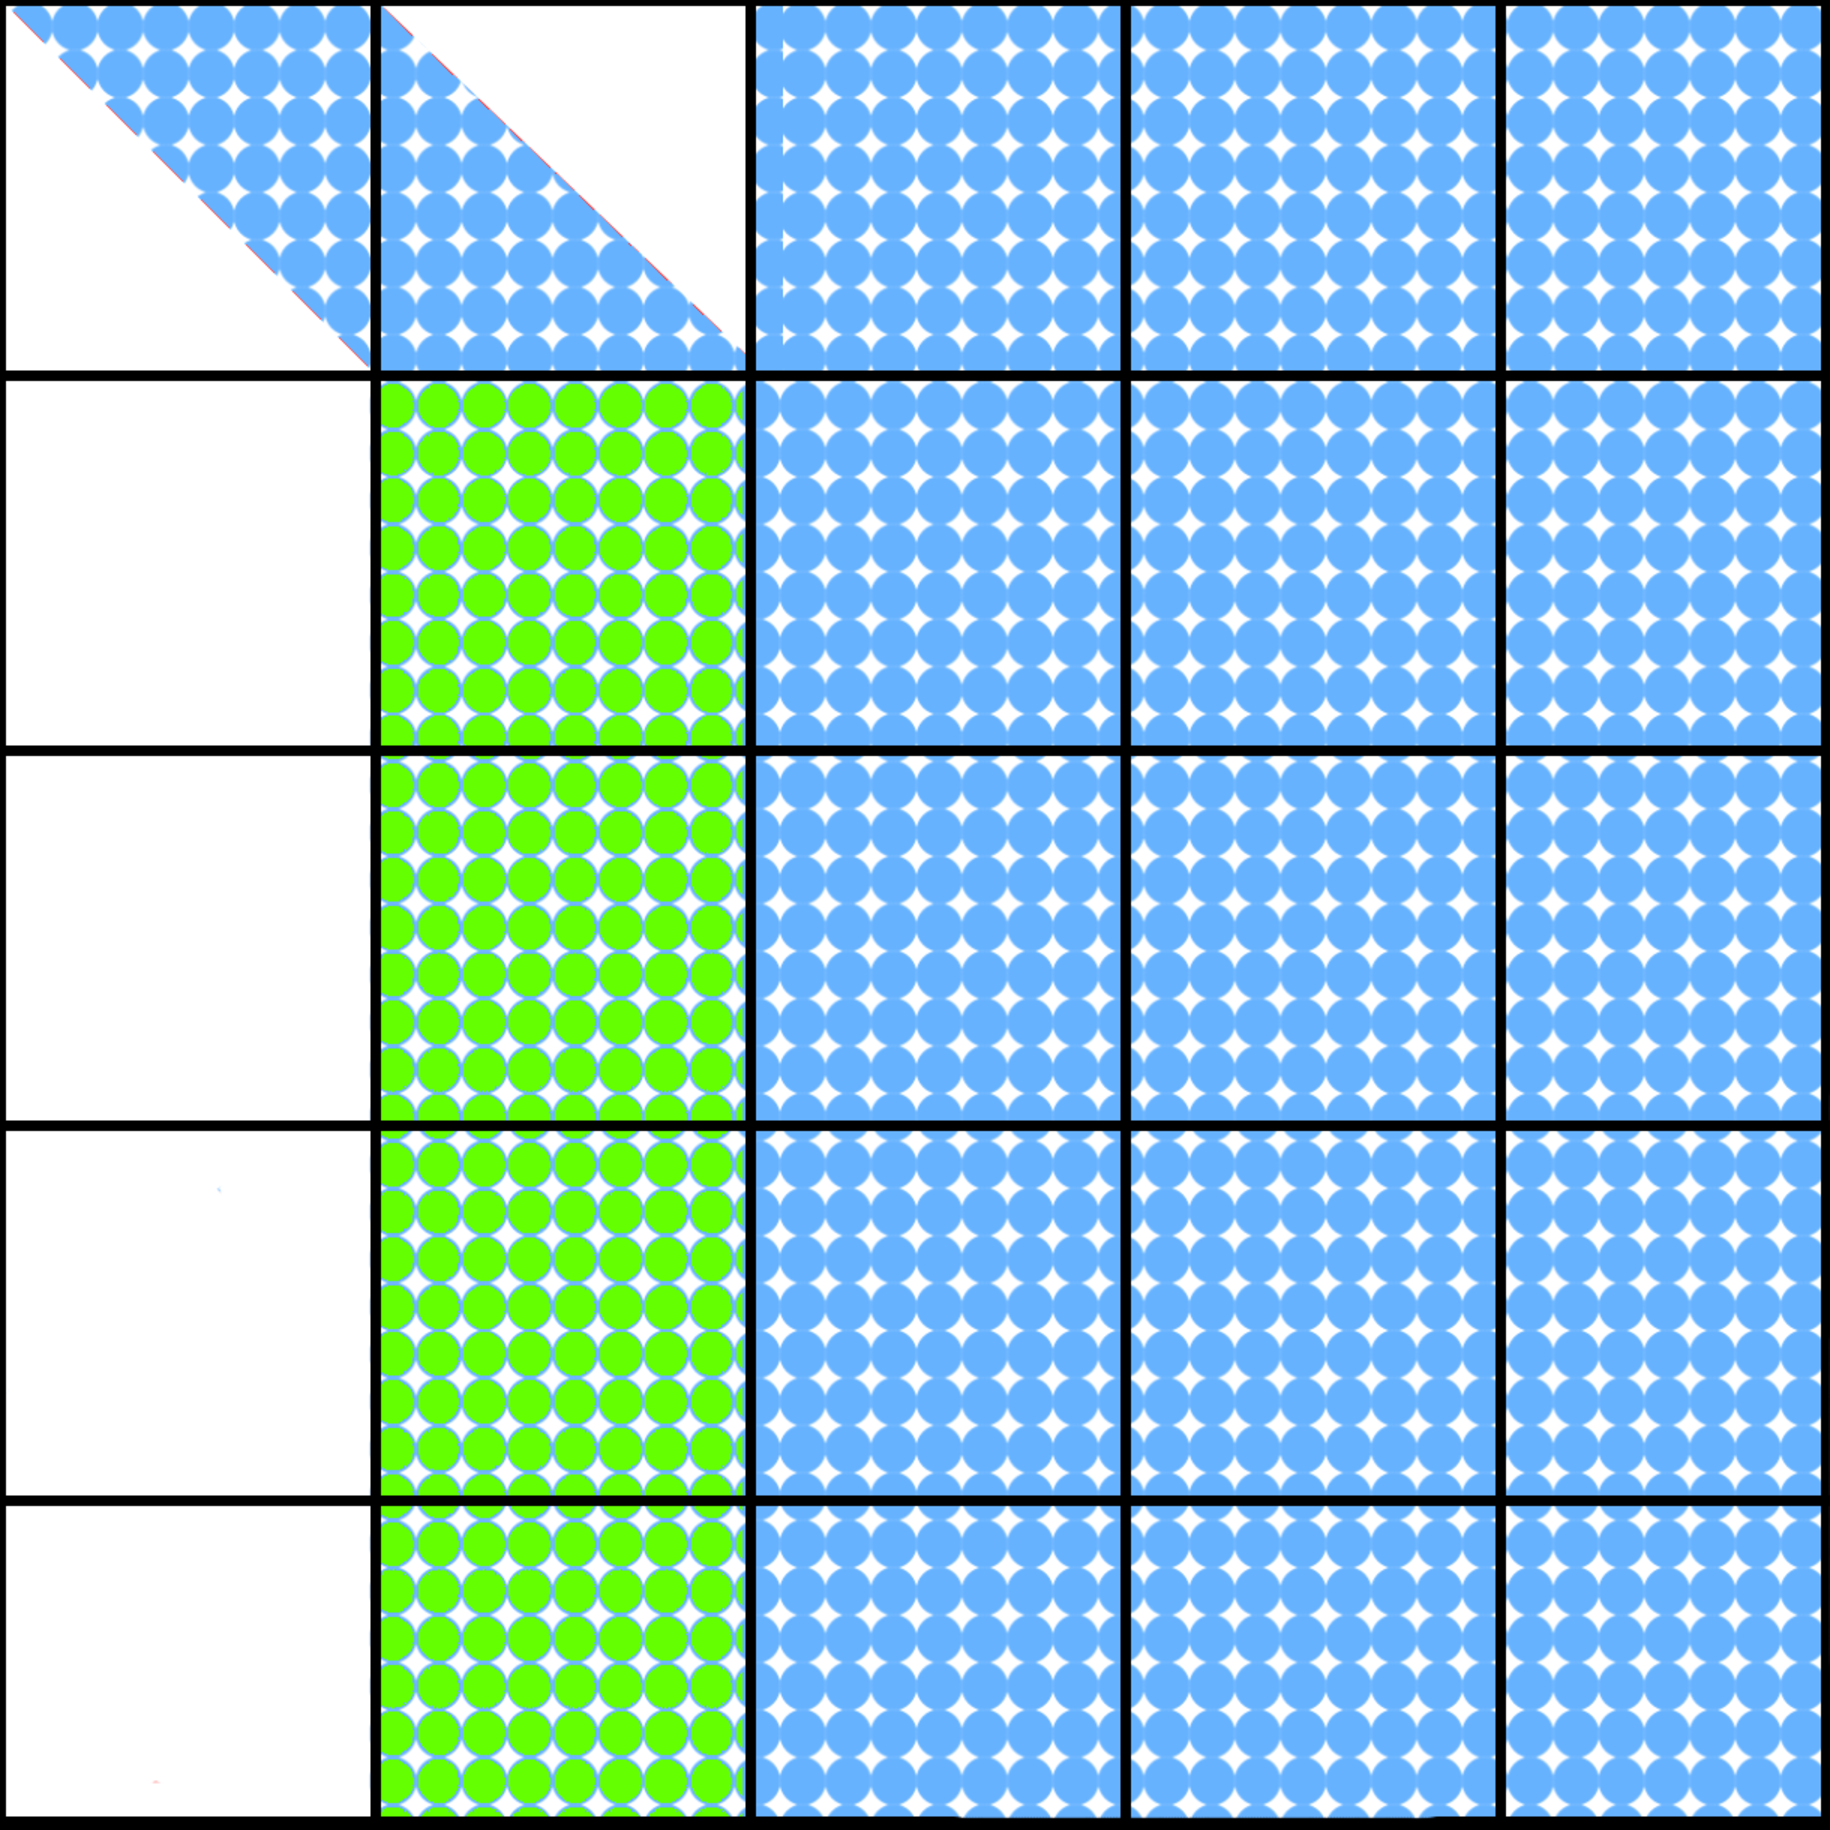
\includegraphics[width=\textwidth]{fig/SVD_tile_8_grid}
      \caption{\label{fig:tile_lq_update_2}Panel update}
  \end{subfigure}
  \hfill
  %%%% 9
  \begin{subfigure}{0.2 \textwidth}
    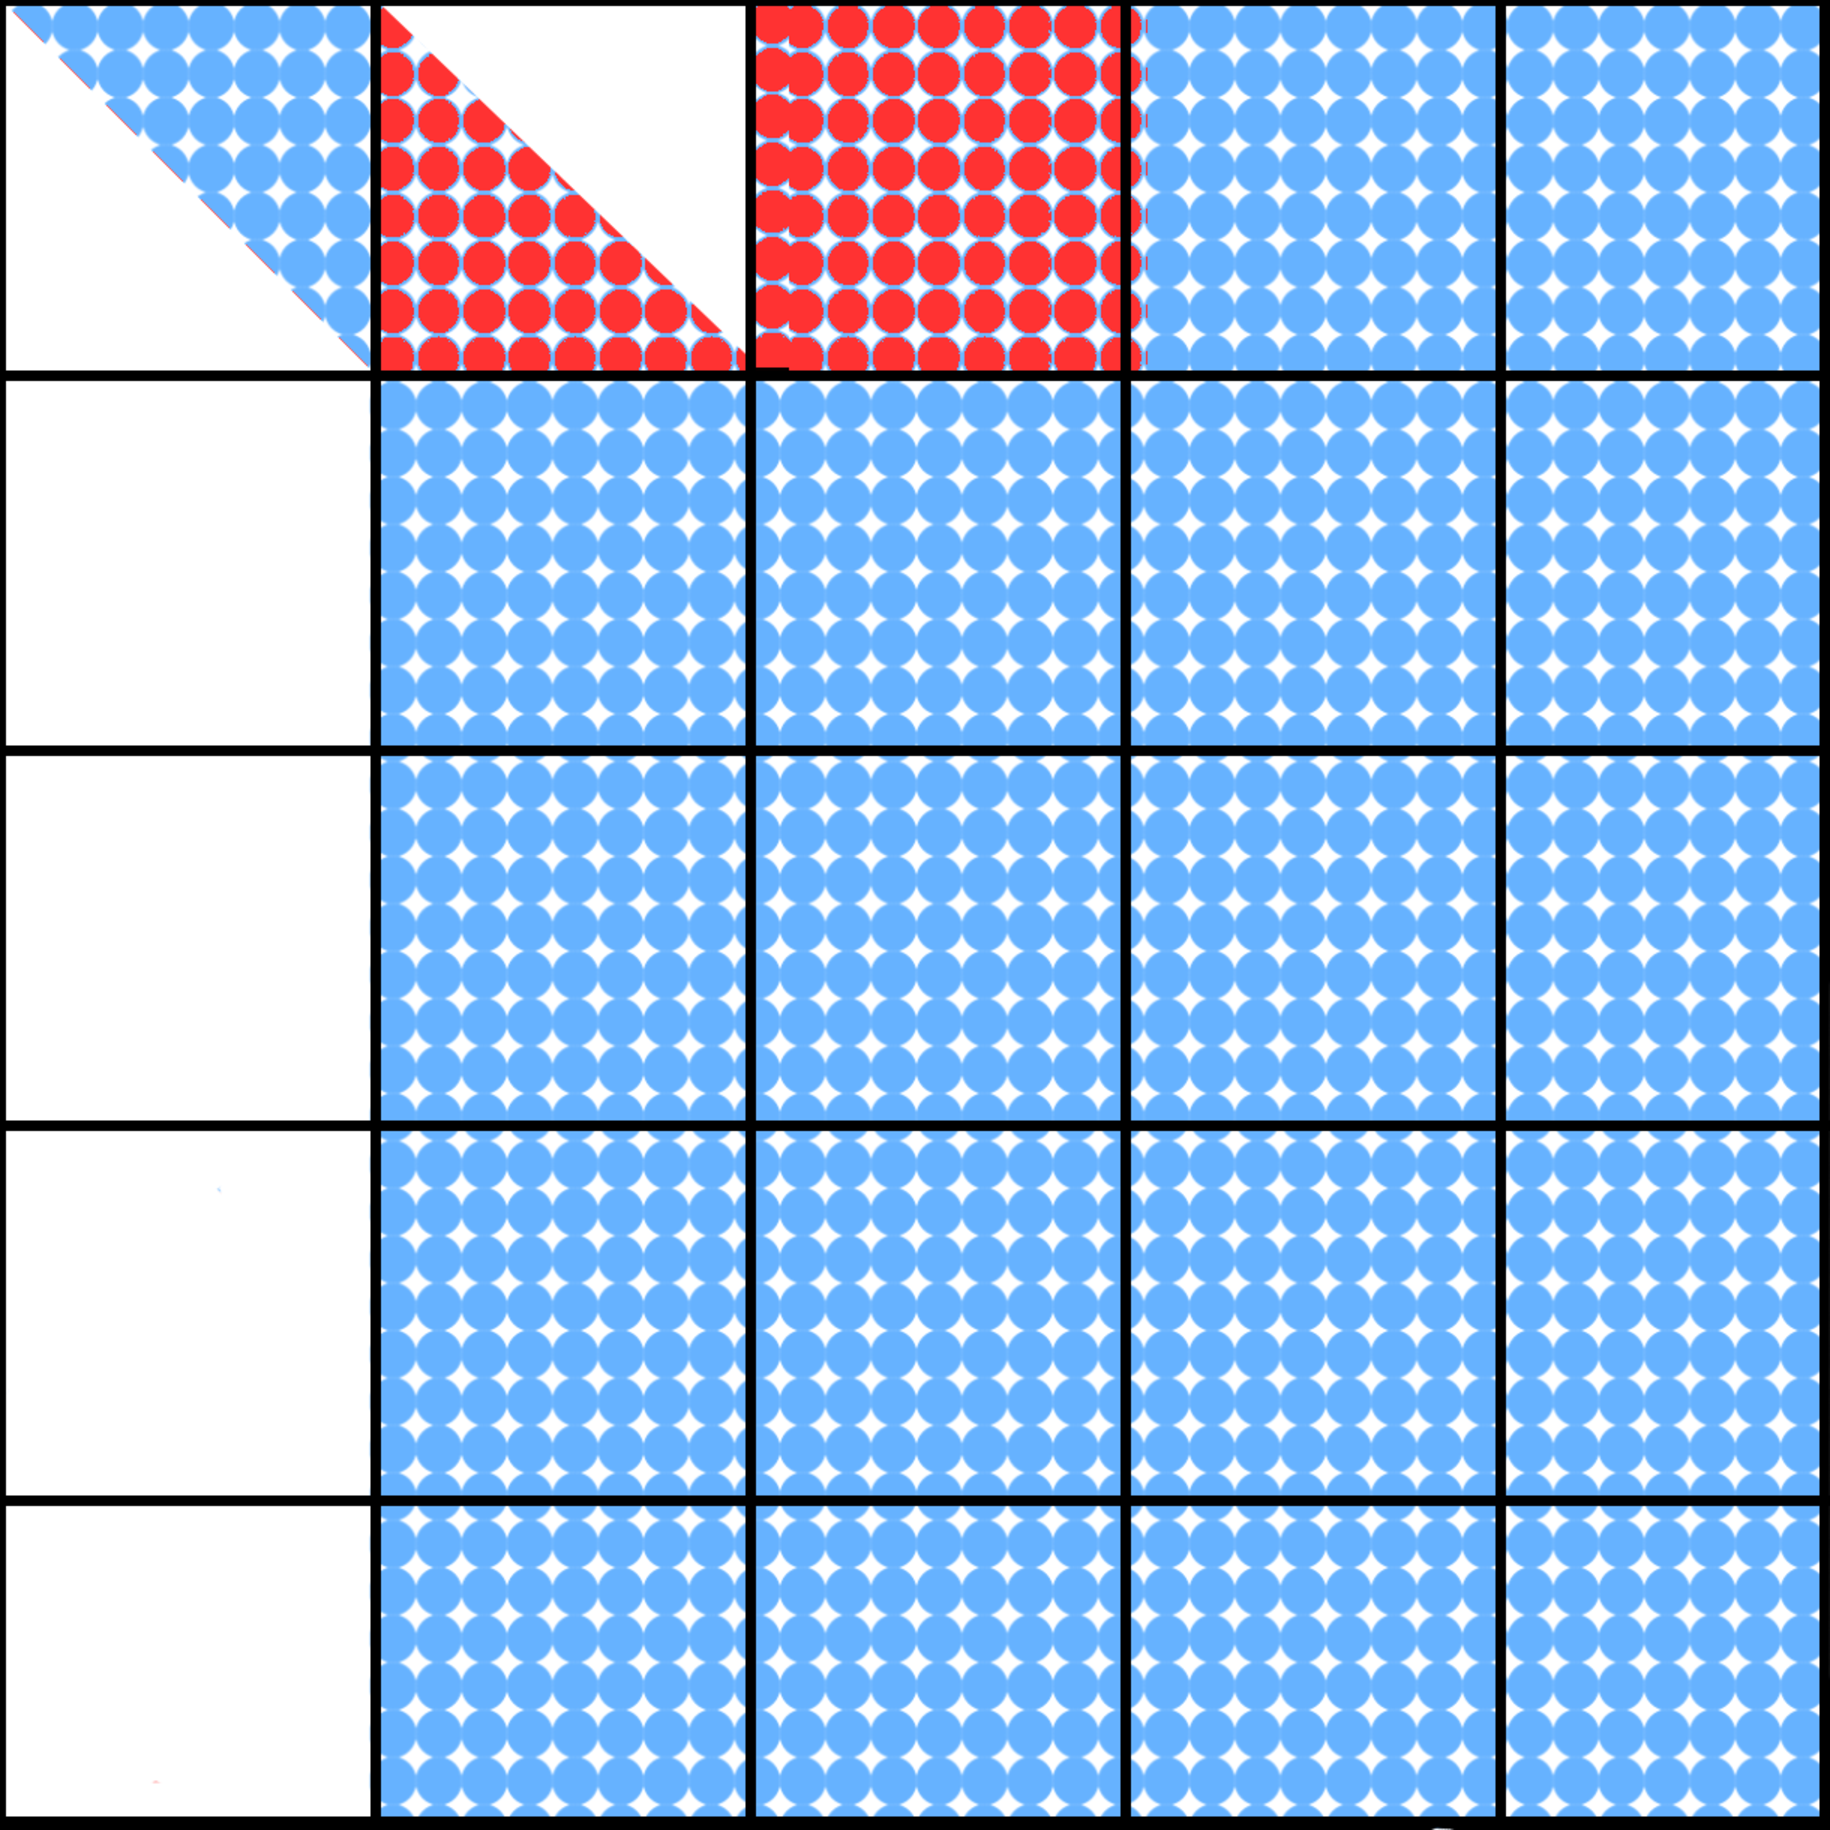
\includegraphics[width=\textwidth]{fig/SVD_tile_9_grid}
    \caption{\label{fig:tile_lq_update_2}TSLQT}
  \end{subfigure}
  \hfill
  %%%% 10
  \begin{subfigure}{0.2 \textwidth}
    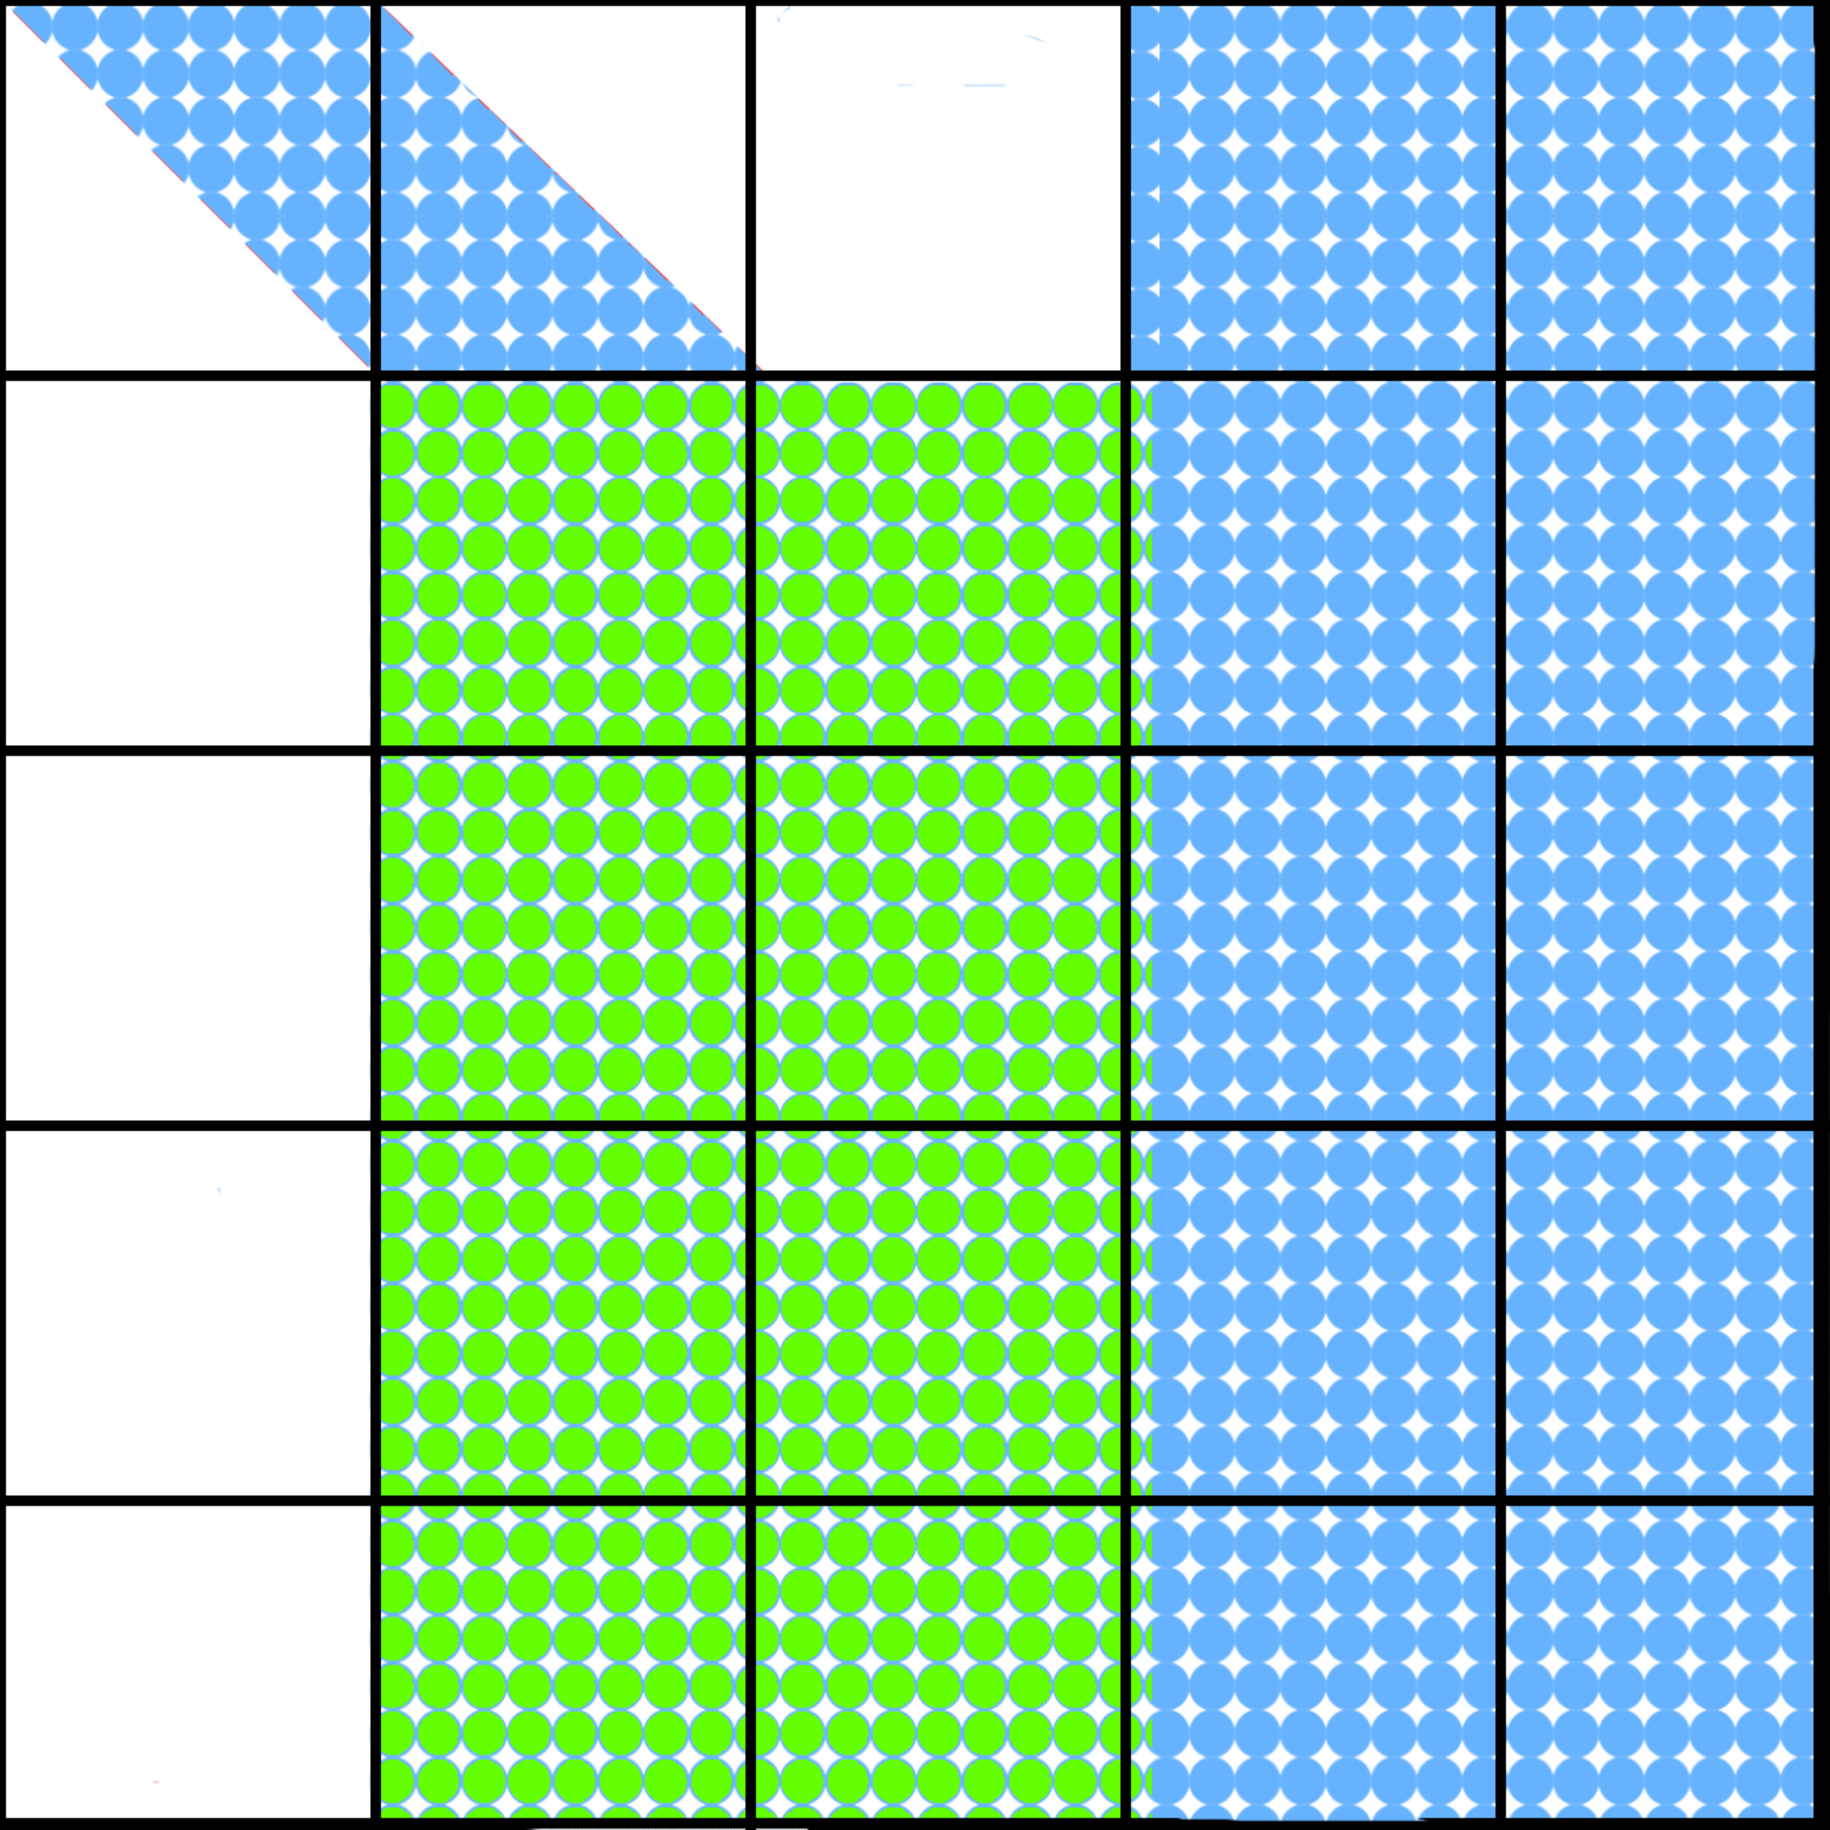
\includegraphics[width=\textwidth]{fig/SVD_tile_10_grid}
    \caption{\label{fig:tile_lq_update_2}Panel update}
  \end{subfigure}
  \hfill
  %%%% 11
  \begin{subfigure}{0.2 \textwidth}
    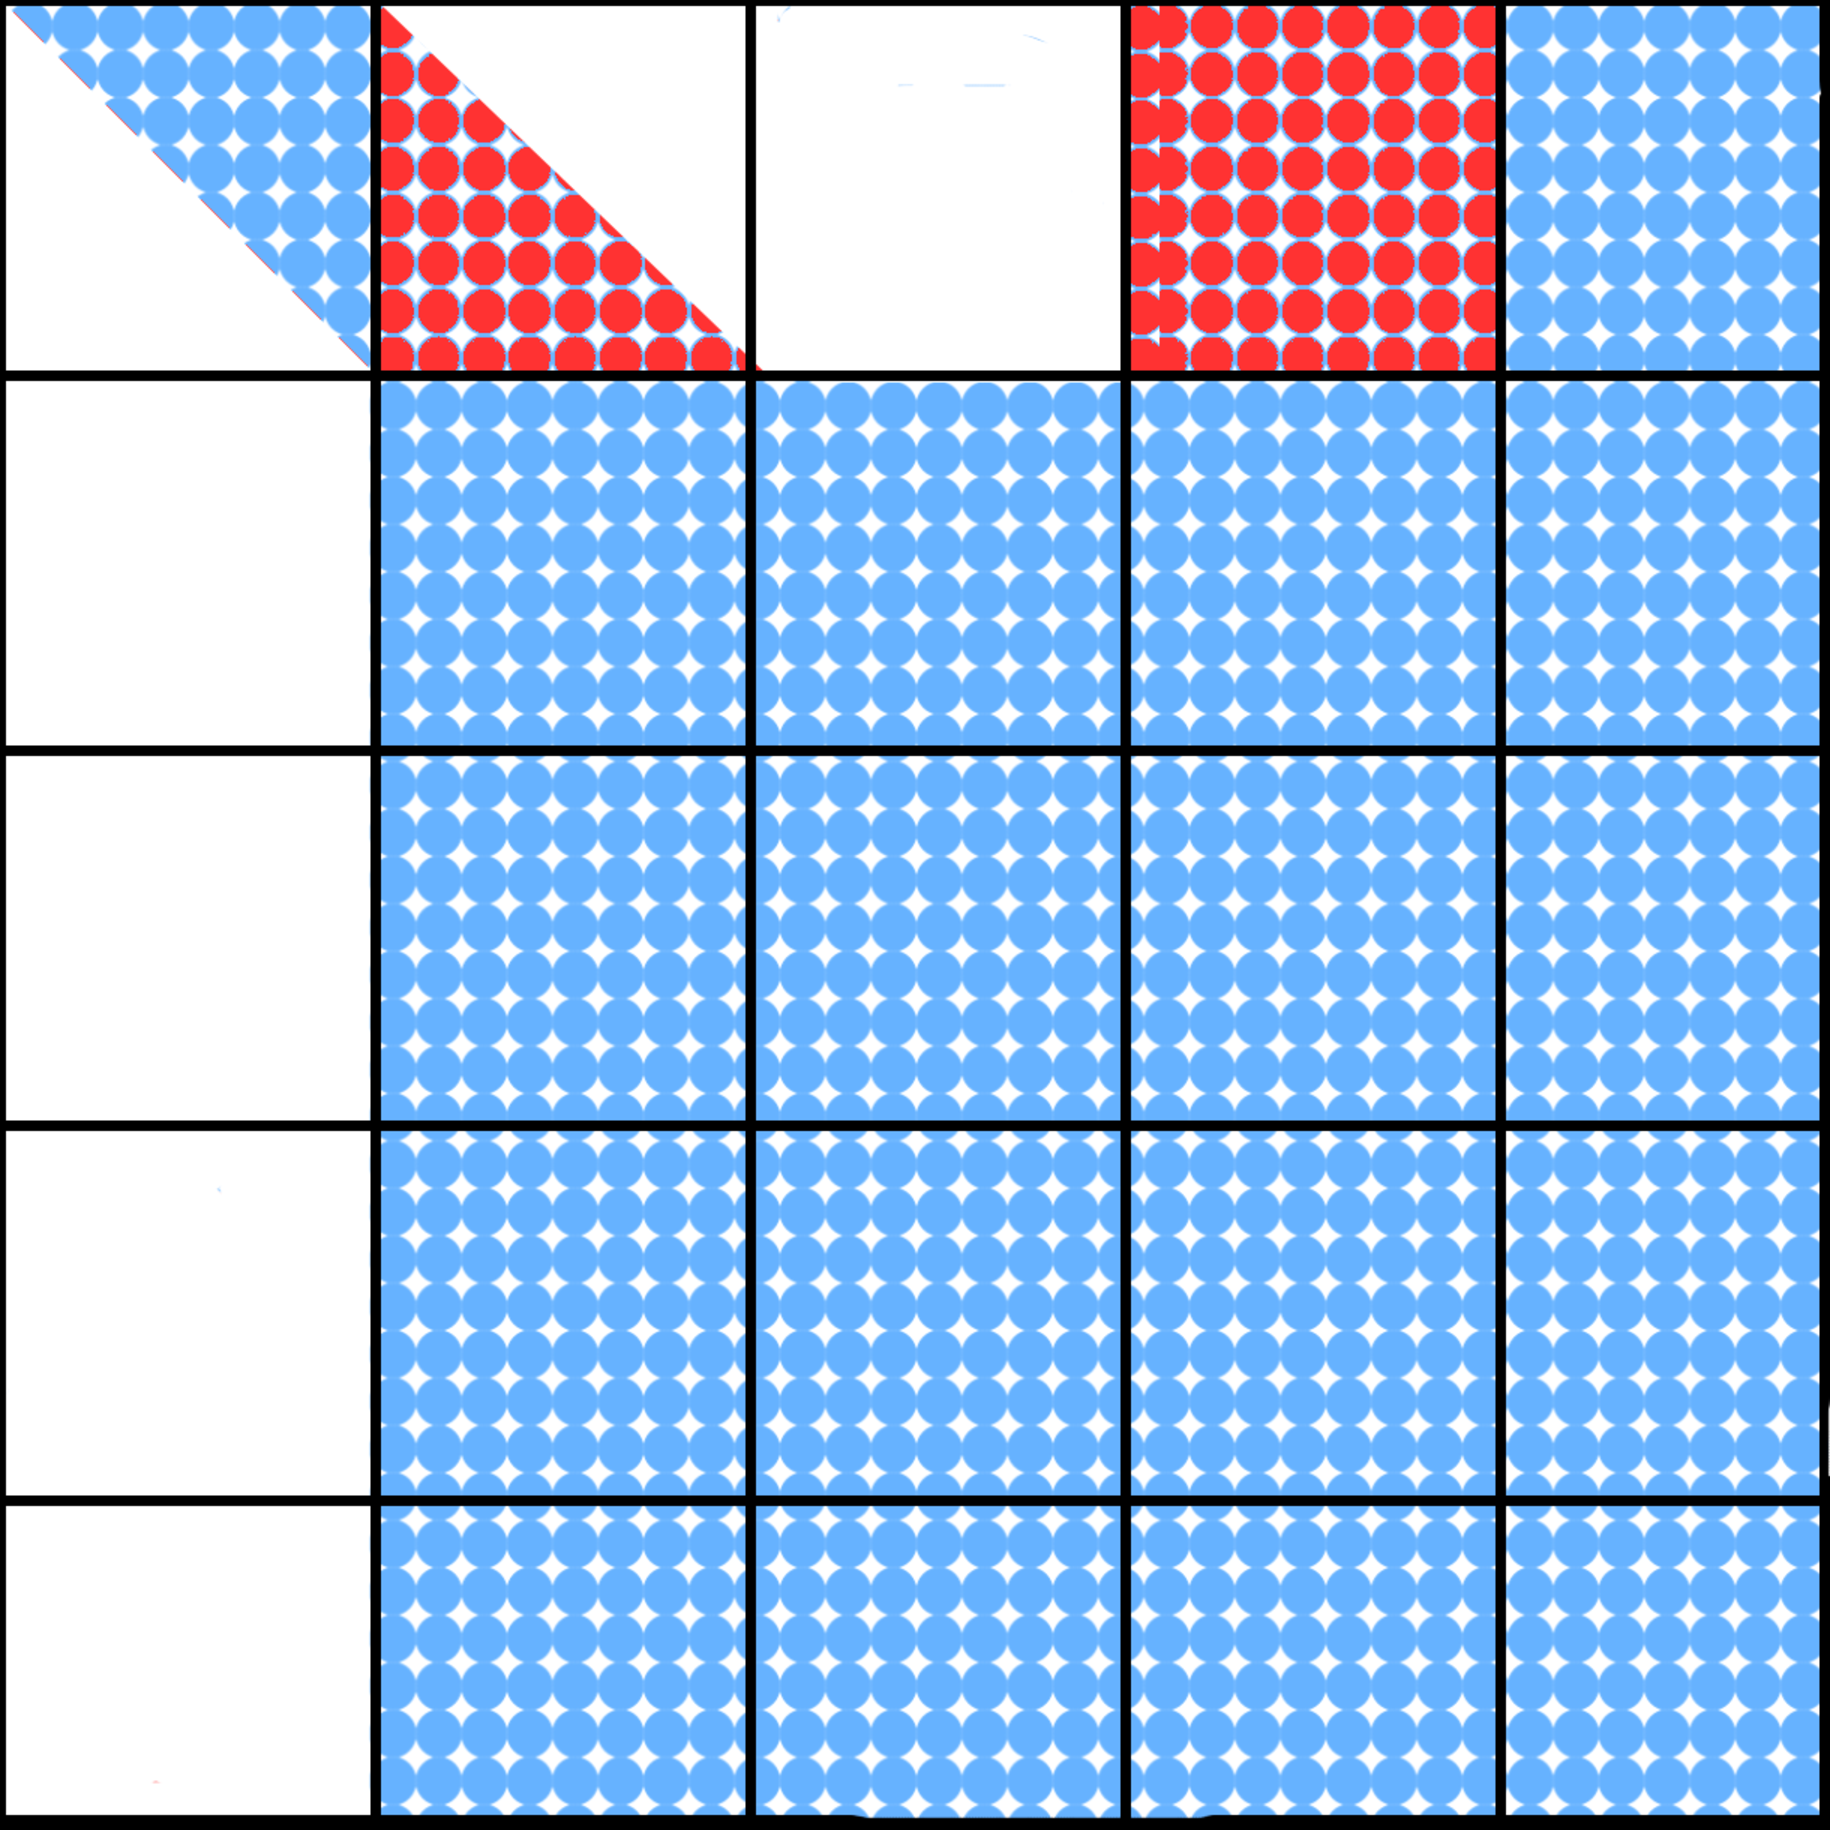
\includegraphics[width=\textwidth]{fig/SVD_tile_11_grid}
    \caption{\label{fig:tile_lq_update_2}TSLQT}
  \end{subfigure}
  \hfill
  %%%% 8
  \begin{subfigure}{0.2 \textwidth}
    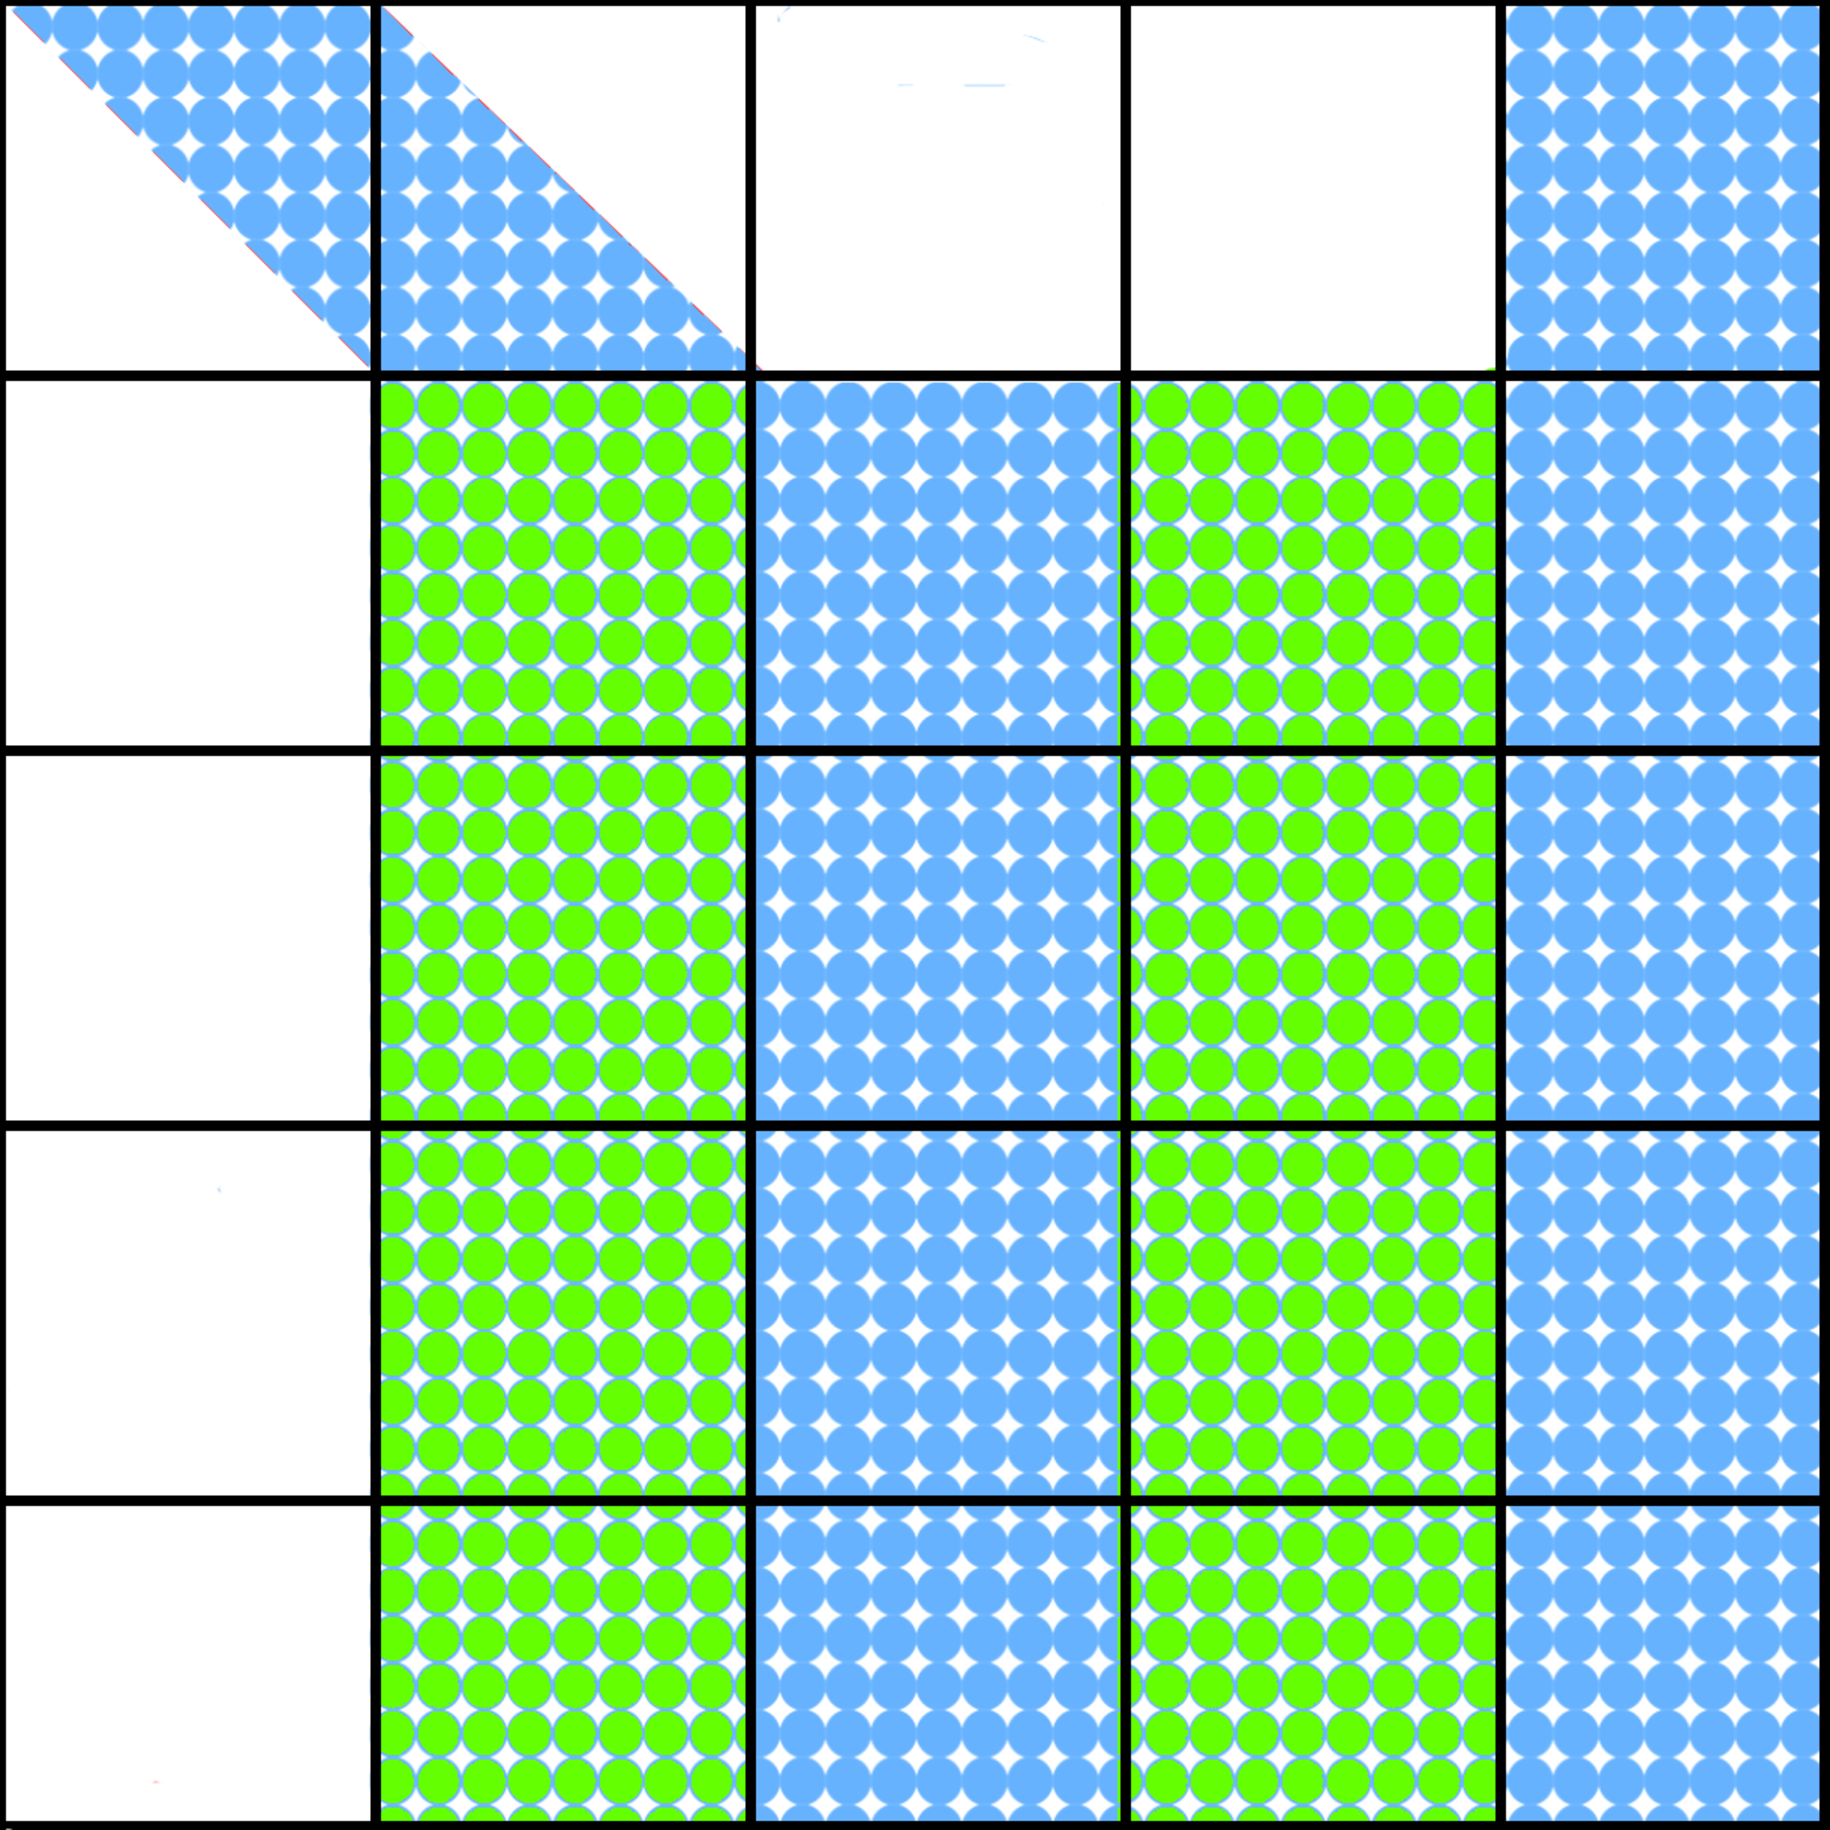
\includegraphics[width=\textwidth]{fig/SVD_tile_12_grid}
    \caption{\label{fig:tile_lq_update_2}Panel update}
  \end{subfigure}
  \hfill

  \caption{Reduction from general matrix to band bidiagonal form
    using early update strategy.
    \label{fig:tile}}
\end{figure}

As illustrated in the DAG (Figure~\ref{fig:dag_tile}),
the early update approach considerably reduces the severity of the
synchronization points.
However,
all the ZUNMQR kernels in charge of updating the
first tile-row have to be completed before starting
any TSQRT kernel,
since the ZUNMQR kernels use the entries of the top left tile and
those entries will be overwritten if any TSQRT kernels are
launched before the end of the first tile-row update.
This explains the bottleneck at TSQRT(2,1) in the DAG.
But the completion of the first TSQRT kernel unlocks many tasks
and leads to high levels of parallelism.


\begin{figure}[h!]
  \begin{center}
    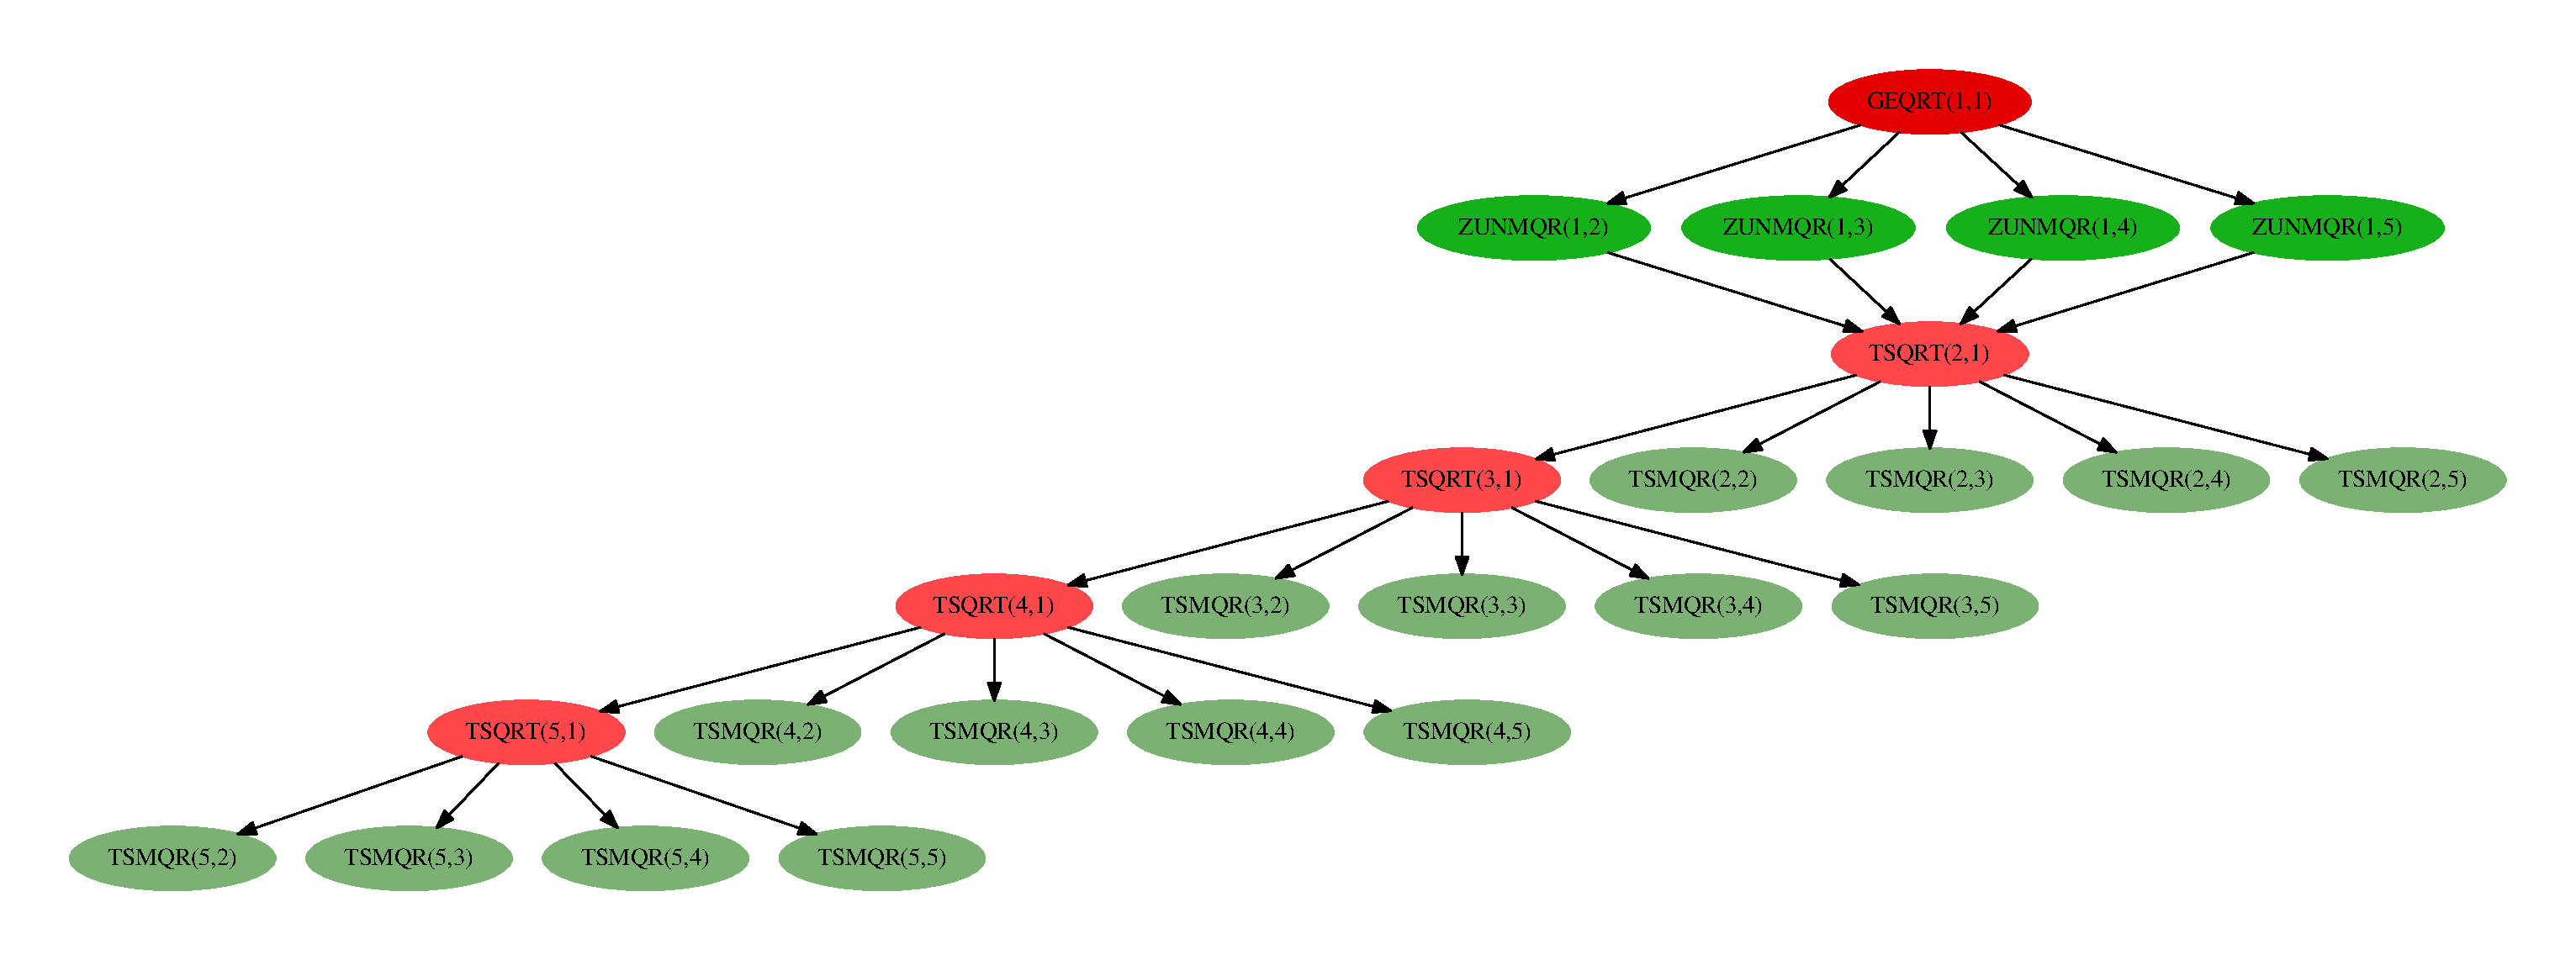
\includegraphics[width=1\textwidth]{fig/dag_tile}
  \end{center}
  \caption{DAG for the early update strategy for band reduction:
    this partial view is limited to the factorization of the first panel and
    the update of the corresponding trailing matrix.}
  \label{fig:dag_tile}
\end{figure}

\subsection{Experimental results}
In order to assess the performance of each strategy,
we design an OpenMP task-based version of each of the two strategies.
In all the experiments within this section,
\texttt{Early update} and \texttt{Late update} will denote
the two strategies explained above, respectively.
We also compare these strategies to the PLASMA 2.8.0 kernel
designed for reduction of a full matrix to band bidiagonal form.
The experiments have been performed with a
NUMA node (two-socket Xeon(R) CPU E5-2650 v3 @ 2.30GHz--Haswell)
and a 68-core
Intel KNL\footnote{https://ark.intel.com/products/94035/Intel-Xeon-Phi-Processor-7250-16GB-1\_40-GHz-68-core}
and all the computations are done in double precision arithmetic.
The performance (Gflop/s) displayed is calculated by dividing the
standard theoretical flops by the time to solution.

\begin{figure}[h!]
  \begin{subfigure}[t]{0.5 \textwidth}
    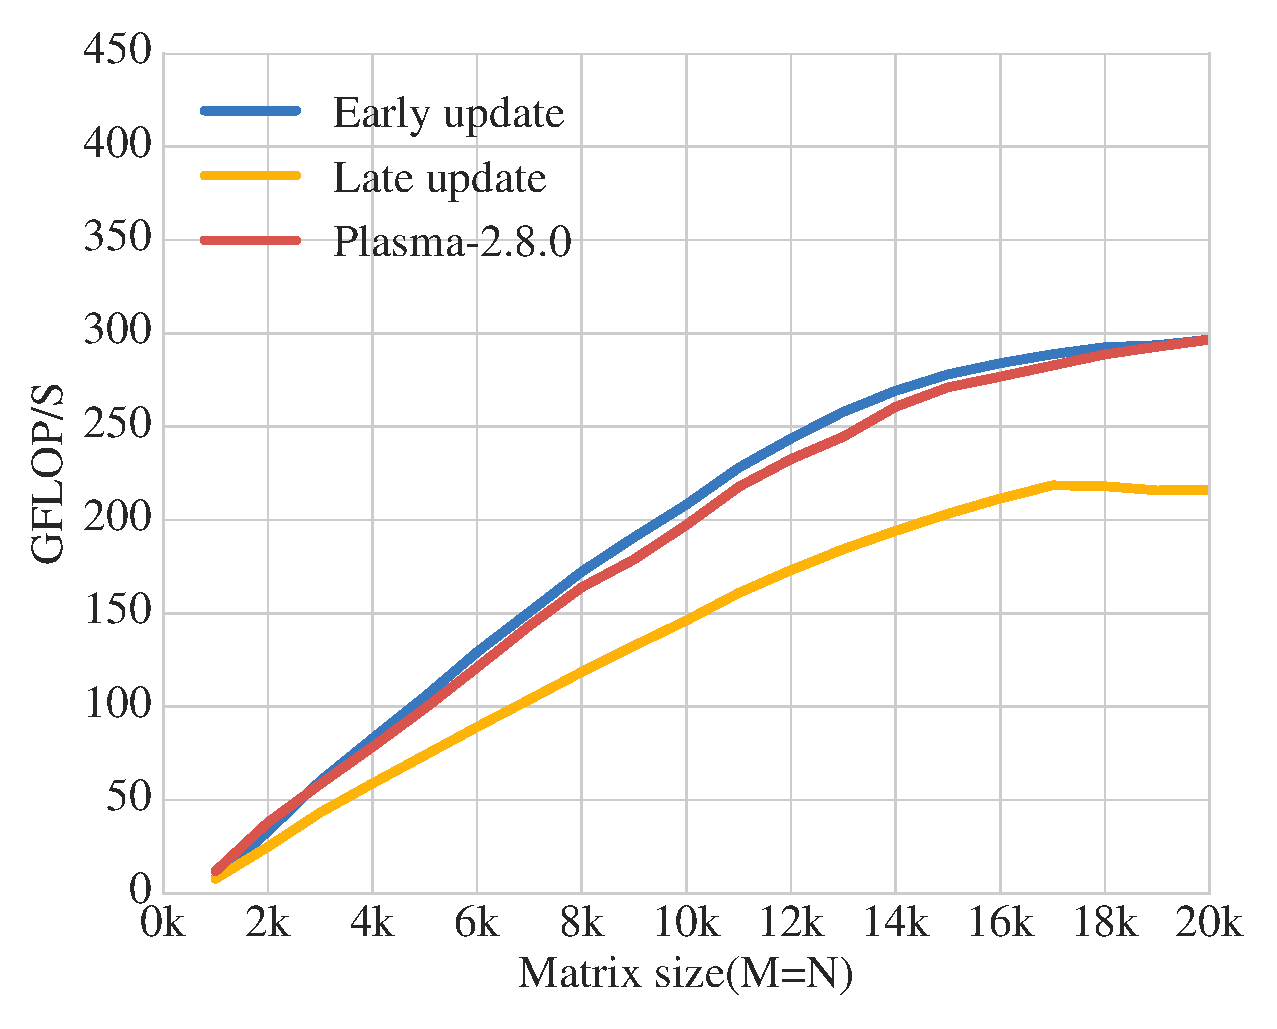
\includegraphics[width=\textwidth]{fig/dge2gb_KNL}
    \caption{\label{fig:dge2gb_DDR4}
      Results with DDR4}
  \end{subfigure}
  \hfill
  \begin{subfigure}[t]{0.5 \textwidth}
    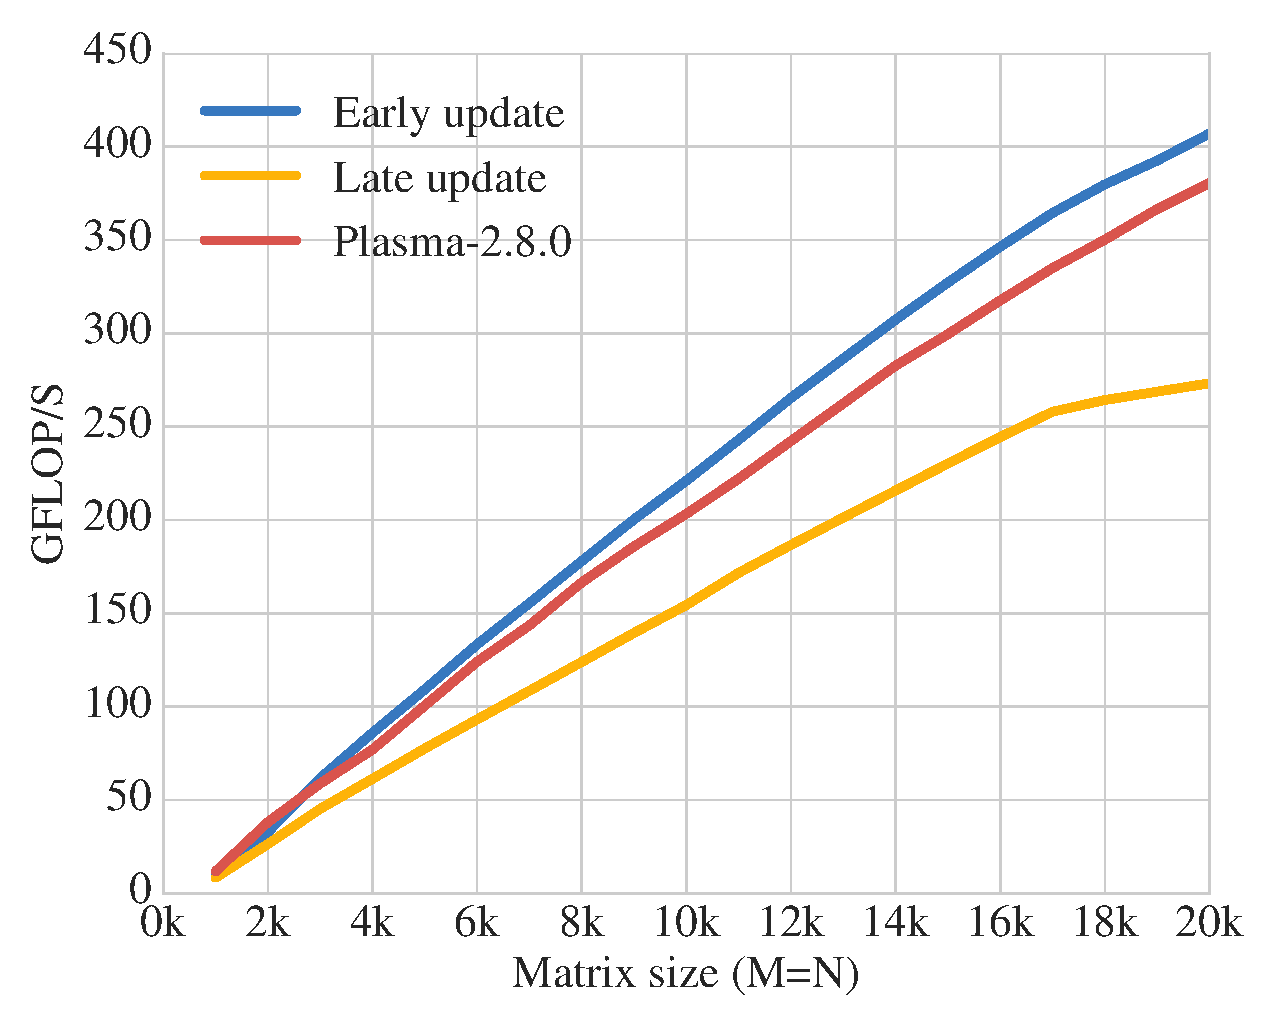
\includegraphics[width=\textwidth]{fig/dge2gb_KNL_HBW}
    \caption{\label{fig:dge2gb_HBW}
      Results with MCDRAM}
  \end{subfigure}
  \caption{Performance comparison of different implementations of
    DGE2GB using $68$ threads on the Intel KNL with square matrices
    ranging in size from $1,000 \times 1,000$ to $20,000 \times
    20,000$.}
  \label{fig:dge2gb_KNL}
\end{figure}


\begin{figure}[h!]
  \begin{subfigure}[t]{0.5 \textwidth}
    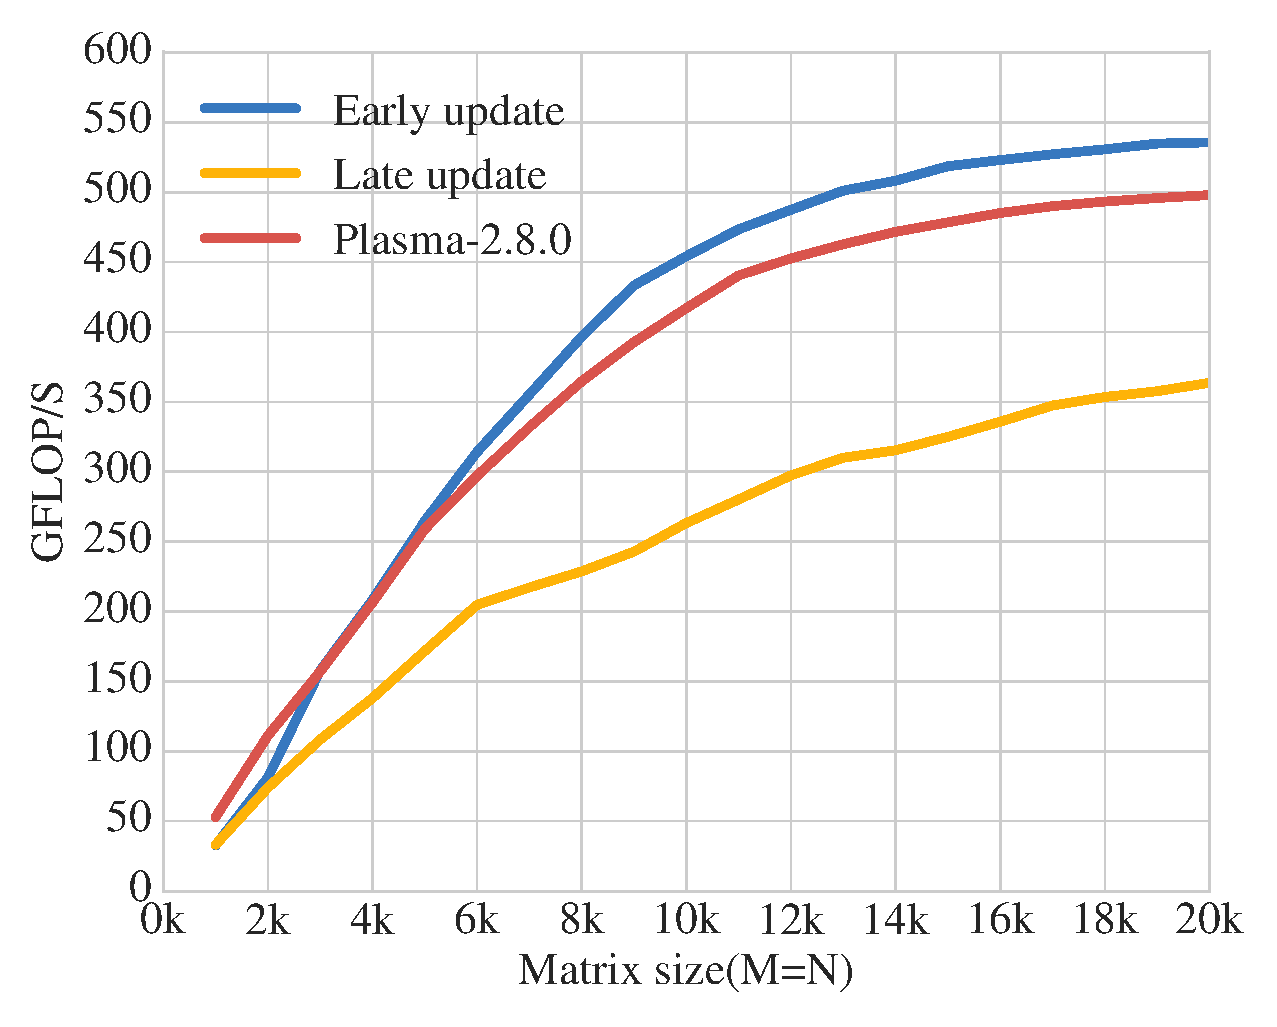
\includegraphics[width=\textwidth]{fig/dge2gb_HASWELL}
    \caption{\label{fig:dge2gb_HASWELL_20}
      Results with 20 threads}
  \end{subfigure}
  \hfill
  \begin{subfigure}[t]{0.5 \textwidth}
    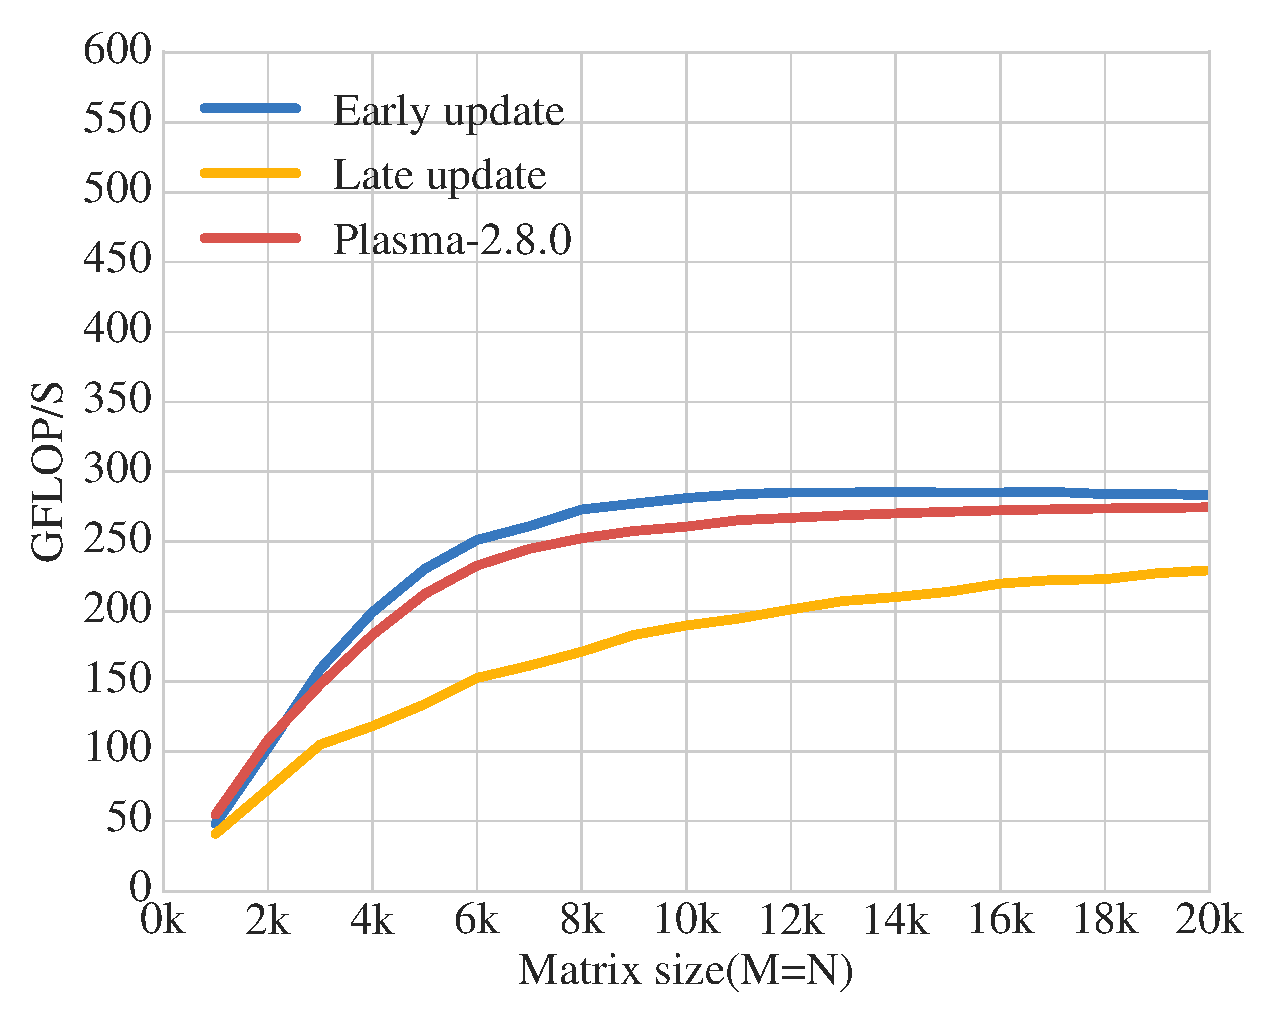
\includegraphics[width=\textwidth]{fig/dge2gb_HASWELL_10}
    \caption{\label{fig:dge2gb_HASWELL_10}
      Results with 10 threads}
  \end{subfigure}
  \caption{Performance comparison of different implementations of
    DGE2GB on a 2x Intel Xeon(R) CPU E5-2650 v3 @ 2.30GHz (20 cores),
    with square matrices ranging in size from $1,000 \times 1,000$ to
    $20,000 \times 20,000$. The experiment with 20 threads is performed
    with the NUMA configuration "numactl --interleave=all" while the
    experiment with 10 threads using only one 10-core socket.}
  \label{fig:dge2gb_HASWELL}
\end{figure}

In addition to the traditional DDR4, the Intel KNL has a high
bandwidth memory called Multi-Channel DRAM (MCDRAM) with a
bandwidth four times greater than the DDR4 bandwidth,
but with a storage capacity limited to 16GB.
There are different configuration options
of MCDRAM, but in this experiment it has been configured
in flat mode i.e. the 16GB memory can be directly allocated from within
an application as is the case for DDR4.
In our experiments we provide results for both DDR4 and MCDRAM.

As illustrated in Figure~\ref{fig:dge2gb_DDR4} where the data is
allocated in DDR4, the early update approach gives the best
performance with a slight advantage over the Plasma-2.8.0
implementation.
The significant gap between the early update and late update
strategies is consistent with our expectations
and confirms the benefit of the early update strategy.
In Figure~\ref{fig:dge2gb_HBW} where data is allocated in
the MCDRAM instead of the regular DDR4, the difference between the
strategies is fairly similar,
although all implementations benefit from the increased memory access
speed.

We obtained a similar result on a NUMA node (2x Intel Xeon(R)
CPU E5-2650 v3) using 20 threads and 10 threads in
Figure~\ref{fig:dge2gb_HASWELL_20} and
Figure~\ref{fig:dge2gb_HASWELL_20} respectively.
However, unlike for the 68-core Intel KNL,
the late update strategy exhibited a more severe
performance penalty.

In the next subsection we investigate ways to remove
the bottlenecks in both synchronisation points in both
the early and late update strategies.

\subsection{Potential improvements}
One way to solve the performance issue discussed for both the
late update and the early update strategy is to revisit the
data dependencies and remove all unnecessary synchronizations.
In Figure~\ref{fig:panel} for example,
since the algorithm is task based,
a part of the trailing matrix update in Figure~\ref{fig:qr_update_1}
could start before the completion of the panel factorization
(Figure~\ref{fig:qr_1}), if its dependencies are satisfied.
In the same way,
once the first tile-row is updated,
the update of the other tile-rows below could follow as
soon as their corresponding tile in the panel is eliminated.
Unfortunately, all these parallelisms are not exploited
in the version presented above.

In fact, the update of the first tile-row uses the top
left corner tile $A(1,1)$ as input (read dependency), while the TSQRT
kernel in charge of the elimination of the square tiles in the panel
modifies $A(1,1)$ (read and write dependency). The update kernel then
waits until the completion of the panel factorization. But a further
analysis of the algorithm helps to realize that as illustrated in
Figure~\ref{fig:rect_panel}, once $A(1,1)$ is factorized, the
elimination operations applied to the rest of the panel modify only
the upper triangular part of $A(1,1)$. On the other hand, the update
of the first tile-row requires only reflectors stored in the lower
triangular part of $A(1,1)$.
Therefore the panel factorization and the update of
the first tile-row could be done in parallel.

Currently our OpenMP implementation supports dependencies only
between full tiles.
This introduces an unnecessary dependency between
the first tile-row update and the first tile-column
elimination through the A(1,1) tile.
To solve this we might want to
split all A(i,i) tiles into upper and lower parts.

Alternatively, one can modify the way OpenMP expresses
its data dependencies.
To illustrate this, lets consider an $nb \times nb$ tile B.
The standard way to express a read or input dependency on B is
\begin{lstlisting}
  #pragma omp task depend(in:B[0:nb*nb])
\end{lstlisting}
while write or output dependency on B would be
\begin{lstlisting}
  #pragma omp task depend(out:B[0:nb*nb]).
\end{lstlisting}

The OpenMP runtime system then ensures that the dependency criteria
are satisfied on each of the $nb \times nb$ entries before executing
the corresponding kernel. But instead of using
\texttt{depend(in:B[0:nb*nb])}, if one uses \texttt{depend(in:B[i])}
the runtime system will check only the $i^{th}$ entry of the tile to
decide whether to execute the kernel or not. Although specifying the
whole ranges is the recommended way, using only a single entry is an
alternative in cases where only some entries of the tile are used and
the $i^{th}$ entry is representative of their dependency. Since the
tile entries are stored in column major format, an input and output
dependency on the upper triangular tile can be simulated by
\texttt{\#pragma omp task depend(inout:B[0])} (zero is the starting
index of the upper triangular tile with respect to C language and
column major storing) and an input dependency on the
lower triangular by \texttt{\#pragma omp task depend(in:B[1])} (one is
the starting index of the lower triangular tile).

Expressing A(i,i) tiles dependency at the upper/lower triangular
granularity helps us achieving a highly parallel kernel as
demonstrated by the corresponding DAG depicted in Figure~\ref{fig:dag_hack}.
\begin{wrapfigure}{r}{0.5\textwidth}
  \begin{center}
    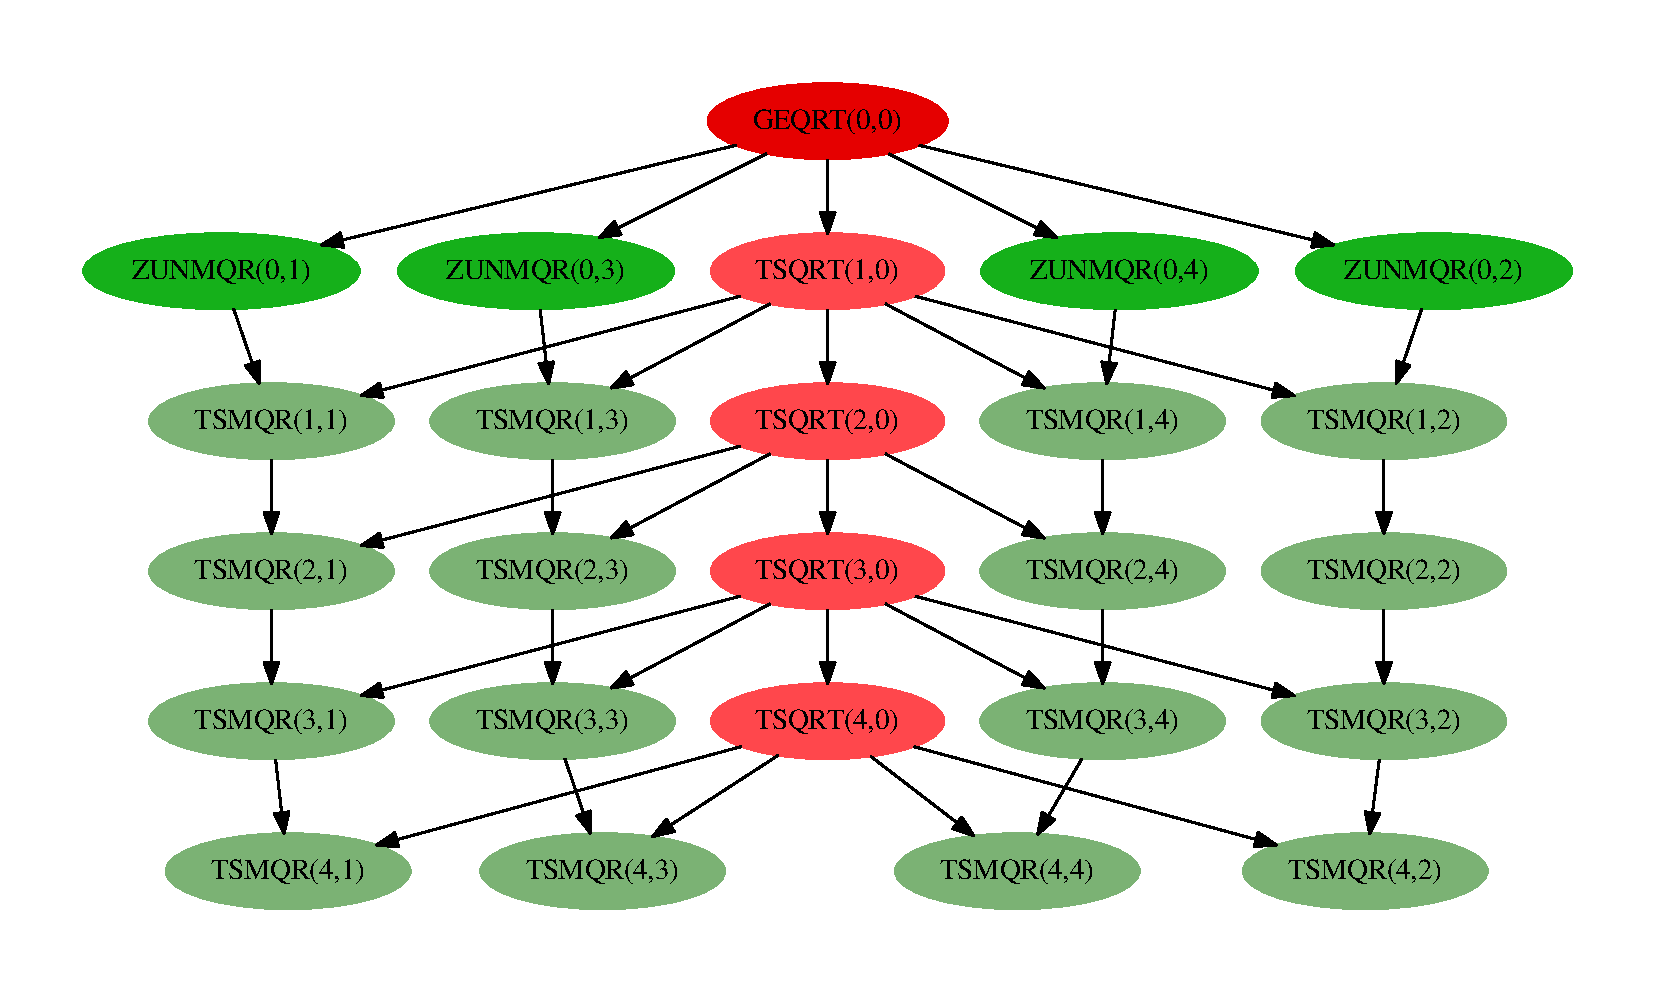
\includegraphics[width=0.48\textwidth]{fig/dag_better}
  \end{center}
  \caption{DAG for the late update strategy for band reduction when
      A(i,i) dependencies are expressed at the upper/lower tile
      granularity. This partial view is limited to the factorization of the
      first panel and the update of the corresponding trailing matrix.}
  \label{fig:dag_hack}
\end{wrapfigure}

We also applied this modification to the early update strategy
to remove the synchronisation point observed previously.
Infact, since we are working at the triangular tile granularity this
releases all unnecessarily dependencies,
the panel and tile strategies should provide comparative results.

To assess the effectiveness of this improvement,
We reproduced the same experiments but now with
some critical dependencies expressed at triangular
tile granularity.

The effectiveness of the modification is illustrated by
the improvement of the Intel 68-core KNL performance
results in Figure~\ref{fig:dge2gb_KNL_HACK} where
the early update and the late update strategies
almost overlap and both are slightly better than Plasma-2.8.0.
This observation is consistent with results with DDR4 as well as
for results with MCDRAM.
There is also a slight improvement in the
performance achieved by the early update strategy
compared to the results in Figure~\ref{fig:dge2gb_KNL} where all dependencies
were expressed at full tile granularity.
We have also observed similar results for the experiments
illustrated in Figure~\ref{fig:dge2gb_HASWELL} with the Intel Haswell NUMA node.


\begin{figure}[h!]
  \begin{subfigure}[t]{0.5 \textwidth}
    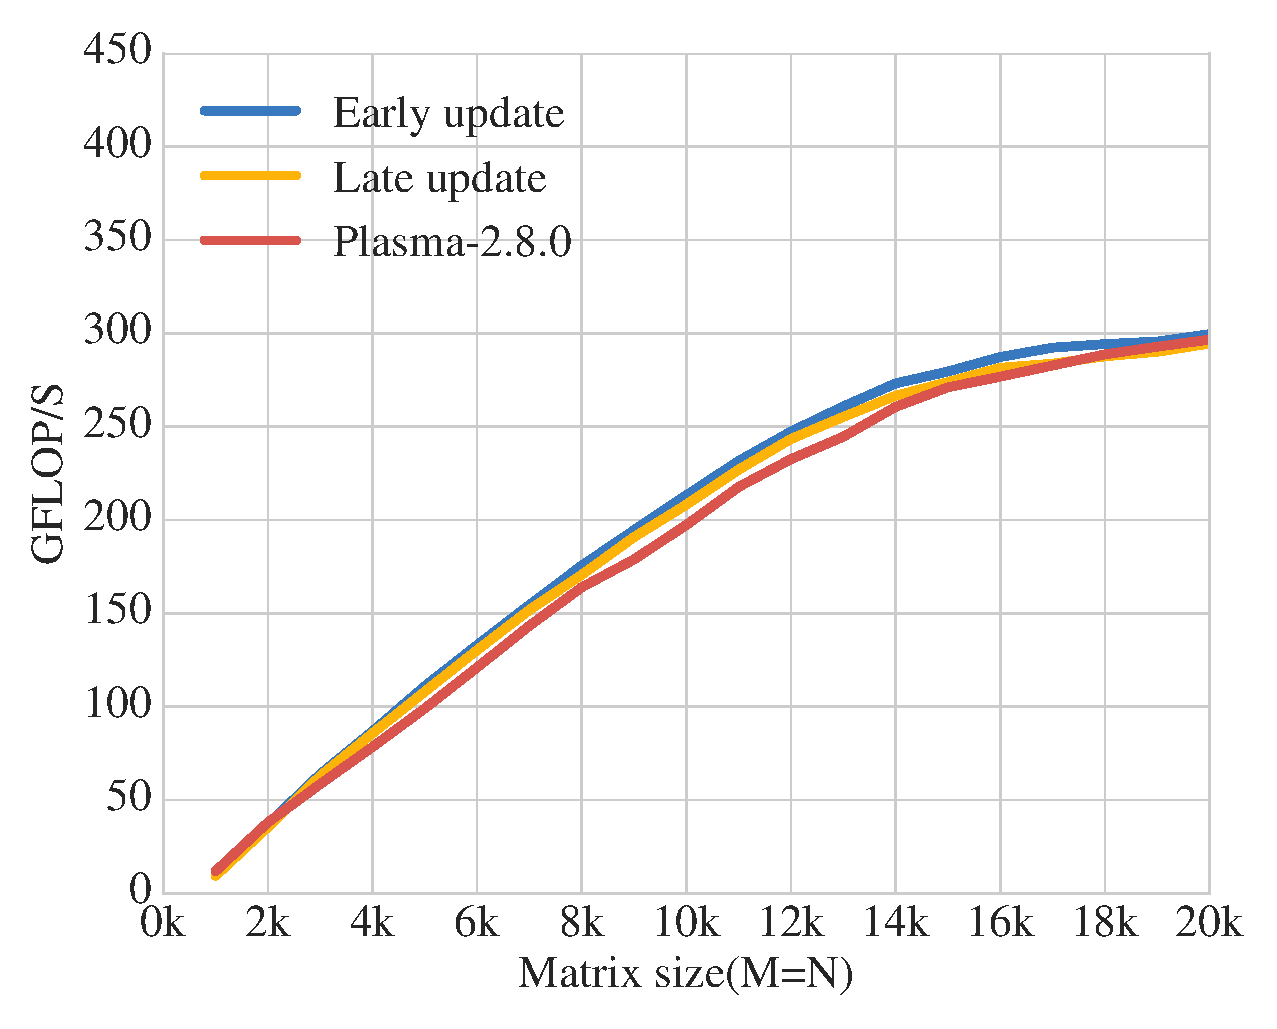
\includegraphics[width=\textwidth]{fig/dge2gb_KNL_HACK}
    \caption{\label{fig:dge2gb_DDR4_HACK}
      Results with DDR4}
  \end{subfigure}
  \begin{subfigure}[t]{0.5 \textwidth}
    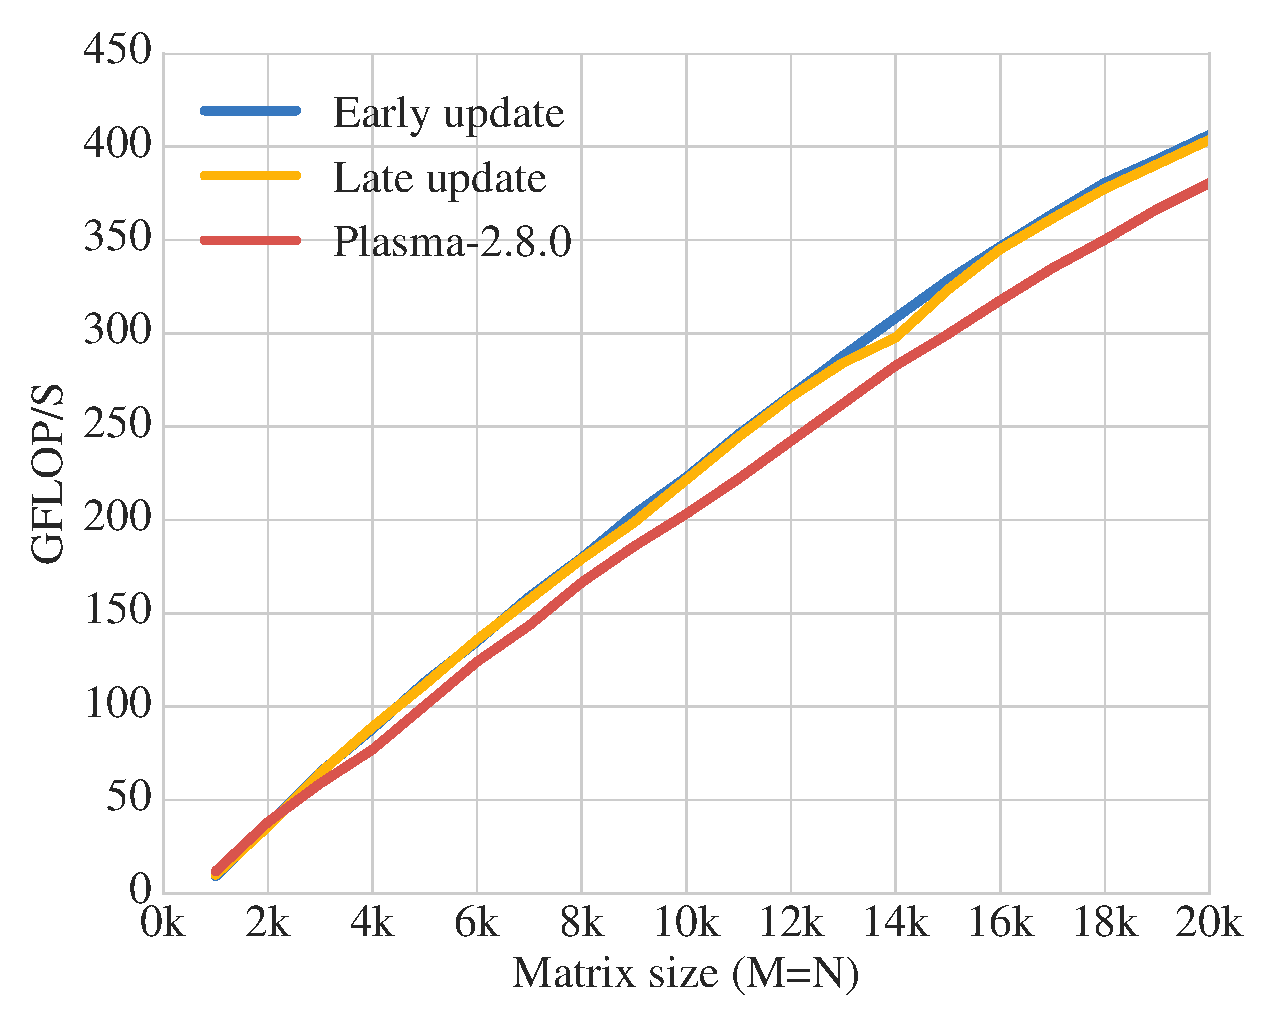
\includegraphics[width=\textwidth]{fig/dge2gb_KNL_HACK_HBW}
    \caption{\label{fig:dge2gb_HBW_HACK}
      Results with MCDRAM}
  \end{subfigure}
  \caption{Performance comparison of different implementations of
    DGE2GB using $68$ threads on the Intel KNL with different
    square matrices ranging in size from $1,000 \times 1,000$ to $20,000 \times 20,000$.
    The code has been modified to  express some
    data dependencies at \texttt{upper/lower triangular tile} granularity.}
  \label{fig:dge2gb_KNL_HACK}
\end{figure}


\begin{figure}[h!]
  \begin{subfigure}[t]{0.5 \textwidth}
    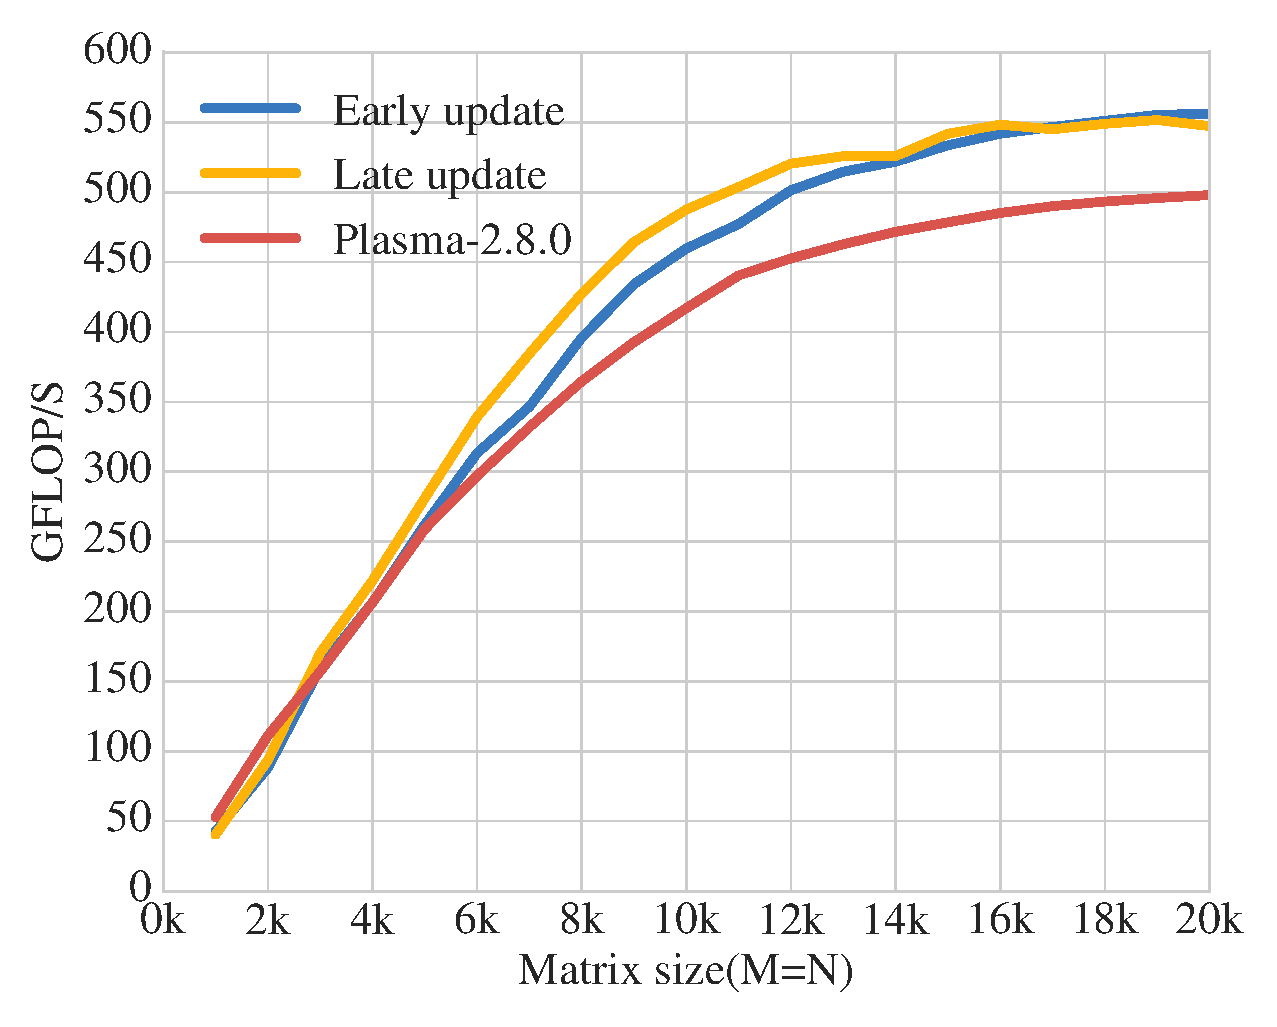
\includegraphics[width=\textwidth]{fig/dge2gb_HASWELL_HACK}
    \caption{\label{fig:dge2gb_HASWELL_20}
      Results with 20 threads}
  \end{subfigure}
  \hfill
  \begin{subfigure}[t]{0.5 \textwidth}
    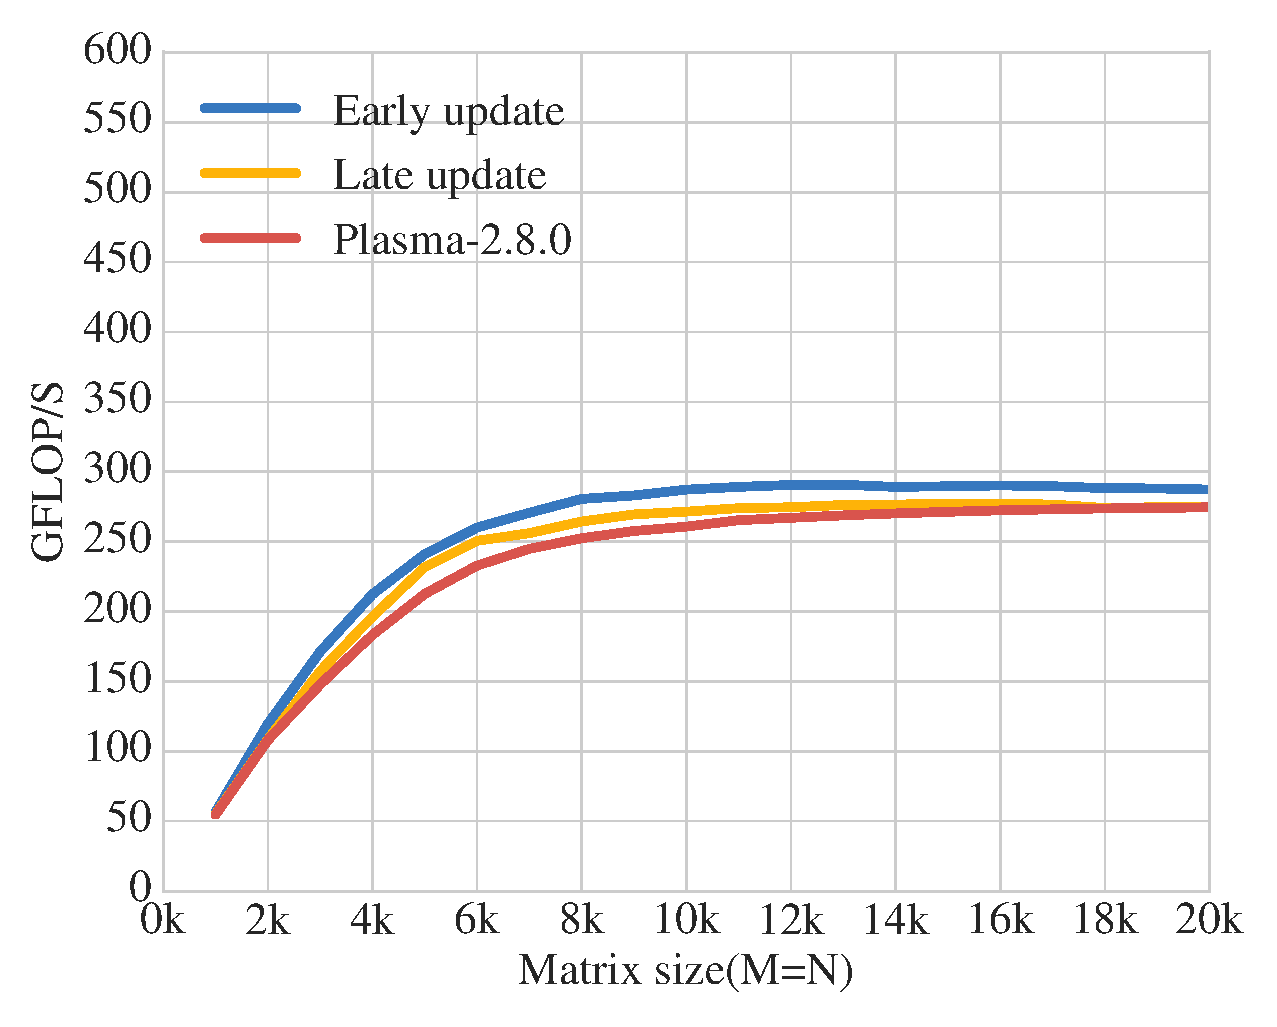
\includegraphics[width=\textwidth]{fig/dge2gb_HASWELL_HACK_10}
    \caption{\label{fig:dge2gb_HASWELL_10}
      Results with 10 threads}
  \end{subfigure}
  \caption{Performance comparison of different implementations of
    DGE2GB on a NUMA node with
    2x Intel Xeon(R) CPU E5-2650 v3 @ 2.30GHz (20 cores),
    with square matrices ranging in size from $1,000 \times 1,000$ to
    $20,000 \times 20,000$. The experiment with 20 threads is performed
    with the NUMA configuration "numactl --interleave=all" while the
    experiment with 10 threads used only one 10-core socket.
    The code has been modified to  express some
    data dependencies at \texttt{upper/lower triangular tile} granularity.}
  \label{fig:dge2gb_HASWELL}
\end{figure}

As reported in~\cite{haidar2013improved},
the SVD implementation based on the
Plasma-2.8.0 bidiagonalization kernel could be two times faster than
Intel’s Math Kernel Library (MKL), when all the singular vectors are
requested and up to 10 times faster if only the singular values are
required. This shows the efficiency of the Plasma-2.8.0 bidiagonalization
kernel, and the performance of our OpenMP implementation
compared Plasma-2.8.0 demonstrates the effectiveness of our prototype.

Furthermore, the hint of working at triangular tile granularity helps
to gain only a slight performance improvement for the early update
strategy while it requires declaring OpenMP dependencies in a
non-conventional way. For this reason, it makes sense to keep the tile
oriented strategy with dependencies at full tile granularity,
as it is reasonably efficient and respects the standard OpenMP programming
conventions.
In addition by declaring data dependencies in a conventional
way the code can be safely extended to a distributed memory environment.

\section{Band reduction to bidiagonal form}\label{sec:bidiag}
In this section we briefly discuss the second stage of the reduction
to bidiagonal form.
In fact the standard bidiagonalization
algorithm as proposed by Golub and Kahan requires $\frac{8}{3}n^3$
flops to reduce an $n \times n$ full matrix to a bidiagonal form.
Similarly, the reduction to block bidiagonal form with a
block size of $nb$ (using $nb \times nb$ tiles) performs
$\frac{8}{3} n\times (n-nb)^2$ flops while the second stage
(moving from block bidiagonal to bidiagonal)
requires only $4 n^2\times nb$ flops~\cite{ltaief2013high}.
Since $nb$ is very small compared to $n$,
the first stage is the dominant part of the algorithm.
However, since the second stage is memory-bound it can penalize the
overall performance if is not implemented efficiently.

We identify two potential solutions for the second stage.
The first consists of using an existing LAPACK routine:
while LAPACK does not provide any routine to reduce a
full matrix to band bidiagonal form,
the GBBRD routine available in LAPACK is designed to
reduce a band matrix to a bidiagonal one.
Relying on a vendor optimized GEBBRD kernel
(for instance Intel MKL), this can be a reasonable solution.

On the other hand, we can implement our own state-of-the-art
solution for the second stage.
In particular we can revisit the cache-aware
and task coalescing techniques introduced by
Haidar~et~al\@.~in~\cite{haidar2011parallel}
which seems to have a good potential for high performance.
We are currently working on an implementation of this
algorithm in OpenMP,
after which we can assess its efficiency by
comparing against the optimized MKL GBBRD kernel.

\section{Concluding remarks}\label{sec:conclusion}
In this paper we have studied different algorithms for
the two-stage bidiagonalization with
a special focus on the first stage:
reduction from a full matrix to a band bidiagonal form.
We proved that even though the late update strategy
is simple to implement and follows the LAPACK-style,
it suffers from numerous synchronisation points that could be
released by the early update approach.

We also discuss potential improvements by relaxing
some OpenMP standard dependency expressing rules.
We demonstrated that while the improvement makes sense for the
late update approach,
the gain is not significant enough for the early update strategy
to sacrifice the robustness of the kernel.
Furthermore,
we have demonstrated the efficiency of our
implementation by showing that it is competitive
with the state-of-the-art kernels.

For the second stage:
reduction of band bidiagonal matrix to bidiagonal form,
we have identified two potential solutions which are
currently in development.

Since this work focused on square matrices,
future work will be devoted to designing specialized kernels
for very tall matrices
(number of rows more than 3x the number of columns)
which require different algorithms to keep the
computational resources working at full efficiency.
Also the current version of our prototype is based on OpenMP,
which is limited to shared memory systems.
In the future,
we will consider using distributed memory runtime
systems such as StarPU~\cite{AugThiNamWac11CCPE} and
PaRSEC~\cite{bosilca2013parsec}
to achieve an extreme-scale, heterogeneous implementation.


\bibliographystyle{unsrt}
\bibliography{svd_biblio}

%%%%%%%%%%%%%%%%%%%%%%%%%%%%%%%%%%%%%%%%%%%%%%%%%%%%%%%%%%%%
% END OF THE ACTUAL DELIVERABLE
%%%%%%%%%%%%%%%%%%%%%%%%%%%%%%%%%%%%%%%%%%%%%%%%%%%%%%%%%%%%

\end{document}
\grid
